\documentclass[11pt,a4paper]{article}

% --- PACKAGES ---
\usepackage[utf8]{inputenc}
\usepackage[T1]{fontenc}
\usepackage{lmodern}
\usepackage[a4paper, top=2.5cm, bottom=2.5cm, left=2.2cm, right=2.2cm]{geometry}
\usepackage{amsmath,amssymb,amsfonts,amsthm,mathtools}
\usepackage{graphicx}
\usepackage[dvipsnames,svgnames,x11names,table]{xcolor}
\usepackage[most]{tcolorbox}
\usepackage{booktabs, tabularx, array, multirow}
\usepackage{fancyhdr}
\usepackage{titlesec}
\usepackage{caption}
\usepackage{microtype}
\usepackage{enumitem}
\usepackage{hyperref}

% --- COLOR DEFINITIONS ---
\definecolor{primary}{RGB}{20, 45, 85}       % Deep Oxford Navy
\definecolor{secondary}{RGB}{35, 95, 160}    % Slate Royal Blue
\definecolor{accent}{RGB}{25, 110, 110}      % Deep Cyan / Teal
\definecolor{boxbg}{RGB}{248, 250, 252}      % Clean Crisp Cool Grey
\definecolor{boxborder}{RGB}{195, 208, 222}  % Slate Border
\definecolor{warningbg}{RGB}{255, 250, 235}  % Warm Amber Background
\definecolor{warningborder}{RGB}{210, 110, 10}% Rich Ochre Border
\definecolor{mathcolor}{RGB}{140, 20, 20}    % Crimson for Key Equations
\definecolor{codebg}{RGB}{240, 243, 246}

% --- TCOLORBOX CUSTOM STYLES ---
\newtcolorbox{analisisbox}[1][]{
  enhanced,
  breakable,
  colback=boxbg,
  colframe=secondary,
  arc=2.5mm,
  boxrule=1pt,
  leftrule=4mm,
  title={\textbf{\sffamily #1}},
  coltitle=white,
  colbacktitle=secondary,
  attach boxed title to top left={yshift=-2mm, xshift=4mm},
  boxed title style={arc=1.5mm, boxrule=0pt},
  fonttitle=\small\sffamily\bfseries,
  top=4.5mm, bottom=3.5mm, left=3.5mm, right=3.5mm
}

\newtcolorbox{teoremabox}[1][]{
  enhanced,
  breakable,
  colback=warningbg,
  colframe=warningborder,
  arc=2mm,
  boxrule=1pt,
  leftrule=4mm,
  title={\textbf{\sffamily #1}},
  coltitle=black,
  colbacktitle=warningborder!25,
  attach boxed title to top left={yshift=-2mm, xshift=4mm},
  boxed title style={arc=1.5mm, boxrule=0pt},
  fonttitle=\small\sffamily\bfseries,
  top=4.5mm, bottom=3.5mm, left=3.5mm, right=3.5mm
}

\newtcolorbox{definisibox}[1][]{
  enhanced,
  breakable,
  colback=accent!5,
  colframe=accent,
  arc=2mm,
  boxrule=1pt,
  leftrule=4mm,
  title={\textbf{\sffamily #1}},
  coltitle=white,
  colbacktitle=accent,
  attach boxed title to top left={yshift=-2mm, xshift=4mm},
  boxed title style={arc=1.5mm, boxrule=0pt},
  fonttitle=\small\sffamily\bfseries,
  top=4.5mm, bottom=3.5mm, left=3.5mm, right=3.5mm
}

\newtcolorbox{studiukasusbox}[1][]{
  enhanced,
  breakable,
  colback=primary!3,
  colframe=primary,
  arc=3mm,
  boxrule=1.2pt,
  leftrule=5mm,
  title={\large\textbf{\sffamily #1}},
  coltitle=white,
  colbacktitle=primary,
  attach boxed title to top left={yshift=-2.5mm, xshift=5mm},
  boxed title style={arc=1.5mm, boxrule=0pt},
  fonttitle=\normalsize\sffamily\bfseries,
  top=5mm, bottom=4mm, left=4mm, right=4mm
}

% --- HYPERREF SETUP ---
\hypersetup{
  colorlinks=true,
  linkcolor=secondary,
  urlcolor=accent,
  citecolor=secondary,
  pdftitle={Buku Ajar Komprehensif Visual Pengolahan Sinyal Digital (PSD) - BAB 1},
  pdfauthor={Muhammad Ayub Rahman},
  pdfsubject={Pengolahan Sinyal Digital Tingkat Lanjut},
  pdfkeywords={DSP, PSD, ADC, Nyquist, SQNR, Multikanal, Kuantisasi, Periodisitas Diskrit, Studi Kasus Terpadu}
}

% --- SECTION FORMATTING ---
\titleformat{\section}
  {\Large\bfseries\sffamily\color{primary}}
  {\thesection}{1em}{}[\titlerule]

\titleformat{\subsection}
  {\large\bfseries\sffamily\color{secondary}}
  {\thesubsection}{1em}{}

\titleformat{\subsubsection}
  {\normalsize\bfseries\sffamily\color{darkgray}}
  {\thesubsubsection}{1em}{}

% --- HEADER & FOOTER ---
\pagestyle{fancy}
\fancyhf{}
\fancyhead[L]{\small\sffamily\color{gray} Buku Ajar Visual Pengolahan Sinyal Digital (PSD)}
\fancyhead[R]{\small\sffamily\color{gray} BAB 1: Fondasi Sinyal \& Pemrosesan Digital}
\fancyfoot[C]{\small\sffamily\thepage}
\renewcommand{\headrulewidth}{0.4pt}
\renewcommand{\footrulewidth}{0.4pt}

% --- DOCUMENT BEGIN ---
\begin{document}

% --- COVER / TITLE HEADER ---
\begin{center}
  \vspace*{0.3cm}
  {\huge\bfseries\sffamily\color{primary} BUKU AJAR VISUAL KOMPREHENSIF}\\[0.3cm]
  {\LARGE\bfseries\sffamily\color{secondary} PENGOLAHAN SINYAL DIGITAL (PSD)}\\[0.4cm]
  {\large\itshape Dari Fisika Sensor \& Transduksi, Formulasi Rantai ASP vs DSP, Konversi Digitalisasi ADC, Teori Kuantisasi \& Kinerja SQNR, Aljabar Sinyal Multikanal-Multidimensi, hingga Analisis Frekuensi Diskrit Tingkat Lanjut}\\[0.4cm]
  \rule{\textwidth}{1.5pt}\\[0.3cm]
  {\Large\bfseries\sffamily\color{primary} BAB 1: Fondasi Pemrosesan Sinyal \& Analisis Gelombang}
  \vspace*{0.3cm}
\end{center}

% --- TABLE OF CONTENTS ---
\begin{tcolorbox}[colback=white, colframe=primary!30, arc=2mm, boxrule=0.8pt]
\tableofcontents
\end{tcolorbox}

\vspace{0.5cm}
\newpage

% =========================================================================
\section{Paradigma Pemrosesan Sinyal — Dari Dunia Fisik Analog (ASP) ke Era Digital (DSP)}
% =========================================================================

\subsection{Dari Fenomena Fisik Menjadi Sinyal Listrik (Peran Sensor \& Transduser)}

Dunia fisis beroperasi berdasarkan besaran-besaran alamiah non-listrik yang bersifat kontinu terhadap ruang dan waktu. Untuk menjembatani dunia analog fisis dengan sistem komputasi terotomatisasi, diperlukan perangkat \textbf{transduser} (elemen pengubah bentuk energi) dan \textbf{sensor} (elemen pendeteksi kuantitas fisik spesifik).

Secara analitis, fungsi transduksi dari suatu sensor riil memetakan besaran fisis masukan $P(t)$ menjadi sinyal tegangan keluaran $v(t)$ melalui hubungan pemodelan matematis:
\begin{equation}
v(t) = \mathcal{S} \cdot P(t) + \beta \cdot P^2(t) + \eta(t)
\end{equation}
di mana $\mathcal{S} = \left.\frac{\partial v}{\partial P}\right|_{P_0}$ merupakan koefisien sensitivitas nominal (*sensitivity factor*), $\beta$ merepresentasikan deviasi non-linieritas orde-2, dan $\eta(t)$ adalah derau termal aditif acak (*Johnson-Nyquist noise*) dengan kerapatan spektral daya:
\begin{equation}
\overline{v_n^2} = 4 k_B T R \Delta f \quad [\text{V}^2]
\end{equation}
dengan $k_B = 1.380649 \times 10^{-23}\text{ J/K}$ (konstanta Boltzmann), $T$ suhu mutlak Kelvin, $R$ resistansi ekuivalen Thévenin sensor, dan $\Delta f$ lebar pita frekuensi pengukuran (*bandwidth*).

\begin{center}
  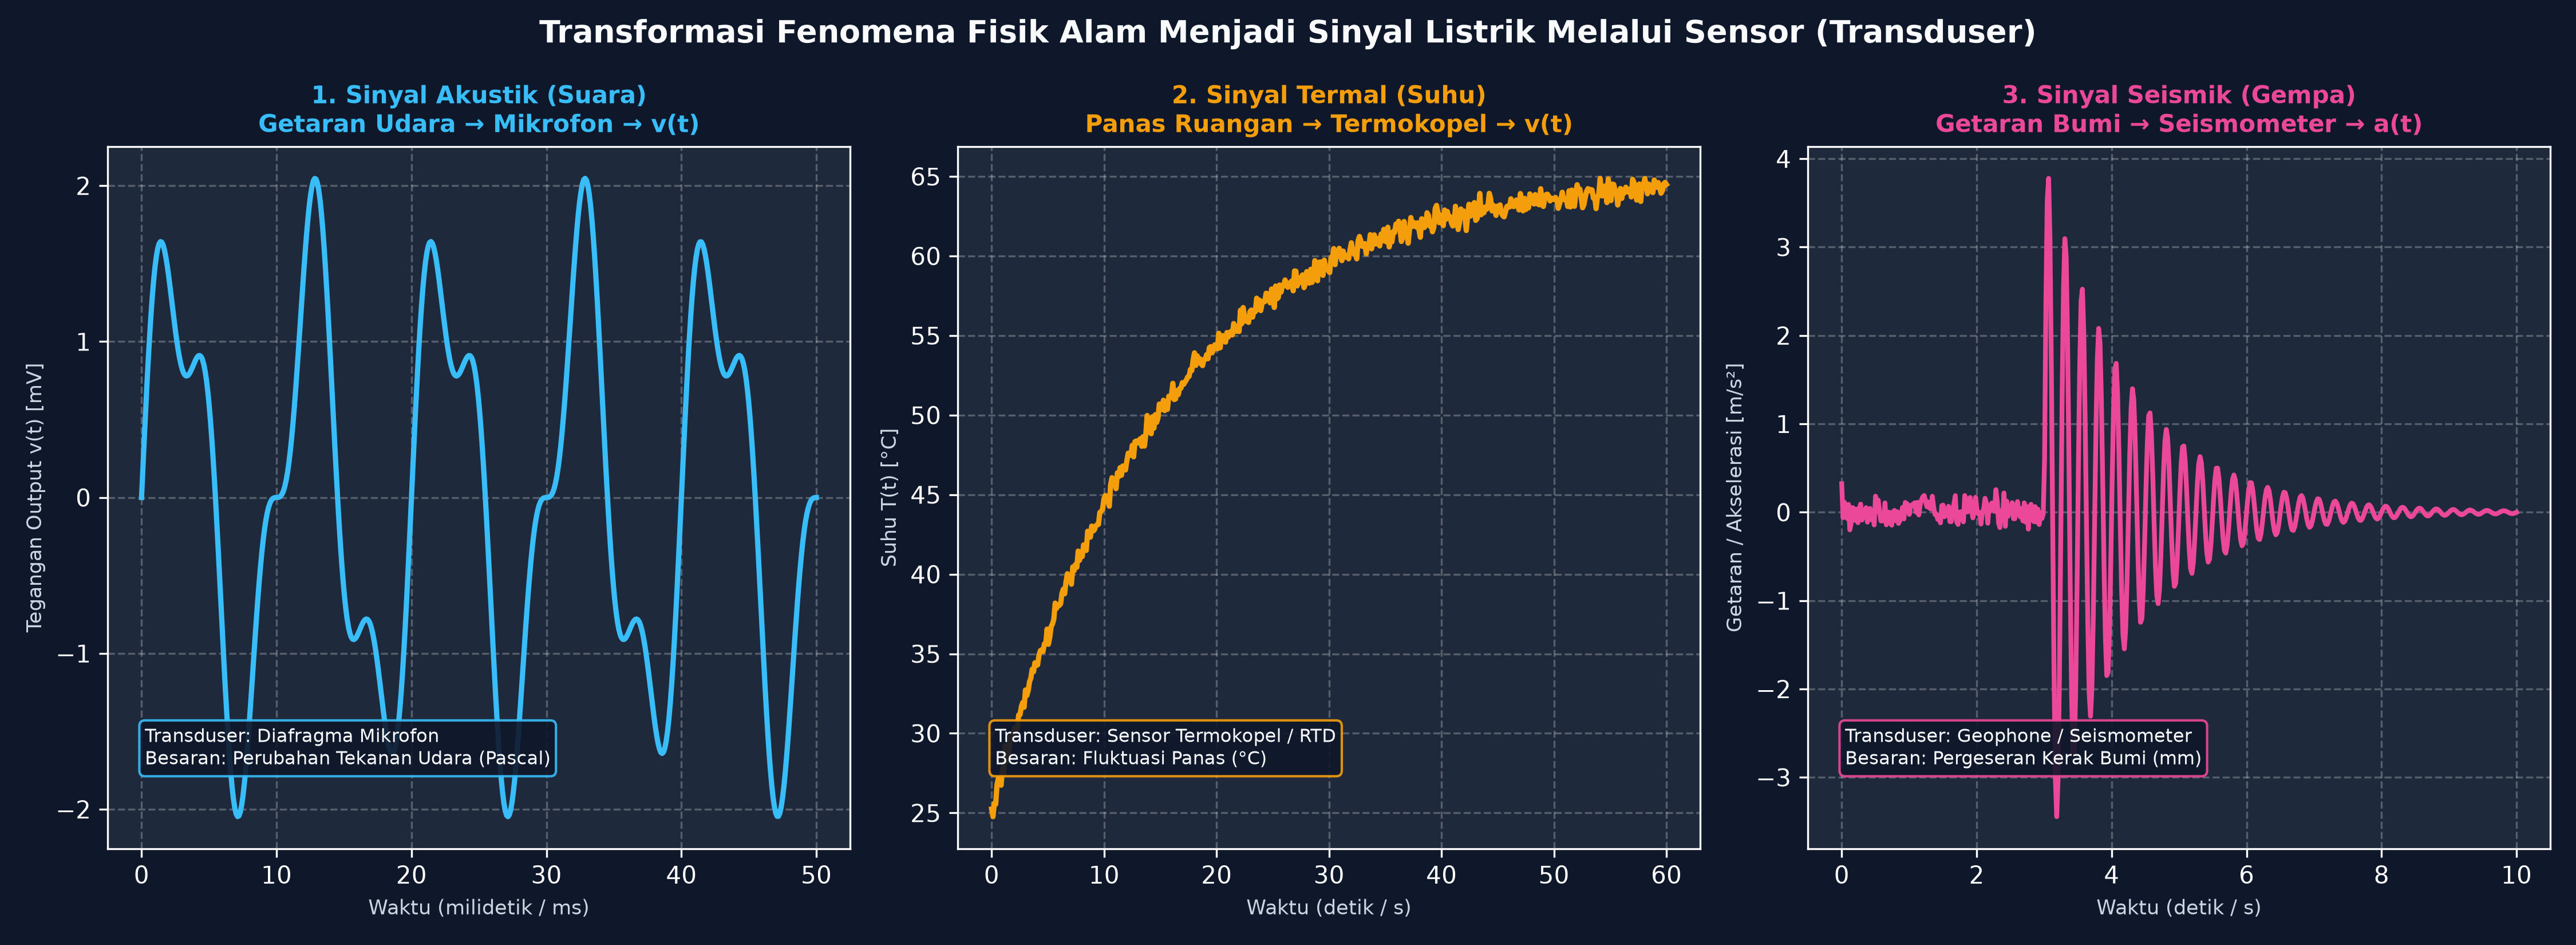
\includegraphics[width=0.92\linewidth]{assets/fenomena_fisik_ke_sinyal.png}
  \captionof{figure}{Konversi analitis fenomena fisis alamiah (Akustik, Termal, Seismik) menjadi fluktuasi sinyal tegangan kontinu.}
\end{center}

\begin{analisisbox}[Dekomposisi Fisik \& Analisis Matematis Tiga Kelas Sinyal]
\begin{enumerate}[leftmargin=*]
  \item \textbf{Panel 1 (Gelombang Akustik / Suara — Biru Muda):}  
  Pita suara manusia menghasilkan gelombang longitudinal tekanan udara $p(x,t)$ yang merambat memenuhi persamaan gelombang Helmholtz 1-D:
  \begin{equation}
  \frac{\partial^2 p(x,t)}{\partial x^2} - \frac{1}{c_s^2}\frac{\partial^2 p(x,t)}{\partial t^2} = 0 \quad (c_s \approx 343\text{ m/s})
  \end{equation}
  Diafragma mikrofon kapasitif mengubah gradien tekanan diferensial $\Delta p(t)$ menjadi perpindahan kapasitansi $\Delta C(t)$, menghasilkan fluktuasi tegangan $v(t) = \frac{Q_0}{C_0^2}\Delta C(t)$ berskala milivolt (mV) dengan spektrum vokal $50\text{ Hz} \le f \le 4\text{ kHz}$.

  \item \textbf{Panel 2 (Dinamika Termal / Suhu — Oranye):}  
  Perpindahan panas pada medium sensor termokopel diatur oleh persamaan difusi Fourier $\frac{\partial T}{\partial t} = \alpha \nabla^2 T$. Respon transien kenaikan temperatur dari $25^\circ\text{C}$ menuju $65^\circ\text{C}$ dimodelkan oleh respon sistem orde-1:
  \begin{equation}
  T(t) = T_{\text{akhir}} + (T_{\text{awal}} - T_{\text{akhir}})e^{-t/\tau_{\text{th}}} + w_{\text{thermal}}(t)
  \end{equation}
  di mana $\tau_{\text{th}} = R_{\text{th}} C_{\text{th}}$ adalah konstanta waktu termal. Tegangan Seebeck yang dihasilkan $v(t) = \alpha_S (T_{\text{hot}} - T_{\text{cold}})$ memperlihatkan riak derau gerigi mikro akibat fluktuasi termal acak.

  \item \textbf{Panel 3 (Percepatan Seismik Kerak Bumi — Magenta):}  
  Gelombang elastisitas sesar tektonik mematuhi persamaan elastodinamika Navier-Cauchy:
  \begin{equation}
  \rho \frac{\partial^2 \mathbf{u}}{\partial t^2} = (\lambda + \mu)\nabla(\nabla \cdot \mathbf{u}) + \mu \nabla^2 \mathbf{u}
  \end{equation}
  Massa seismometer menghasilkan gaya inersia $F(t) = -m \ddot{x}_g(t)$ yang ditransduksikan menjadi lonjakan akselerasi tajam hingga $+3.8\text{ m/s}^2$ pada saat $t = 3.0\text{ s}$ dan meluruh secara sinusoidal teredam (*damped harmonic oscillation*):
  \begin{equation}
  a(t) = A_0 e^{-\zeta \omega_n (t - t_0)} \sin\left(\omega_n \sqrt{1 - \zeta^2}(t - t_0)\right) u(t - t_0)
  \end{equation}
\end{enumerate}
\end{analisisbox}

\vspace{0.3cm}
\subsection{Paradigma Pemrosesan: Rantai ASP (Analog) vs Rantai DSP (Digital)}

Pemrosesan sinyal bertujuan mentransformasikan sinyal masukan $x(t)$ untuk menghilangkan derau, mengekstraksi parameter kunci, maupun mengubah domain informasi menjadi sinyal keluaran $y(t)$.

\begin{center}
  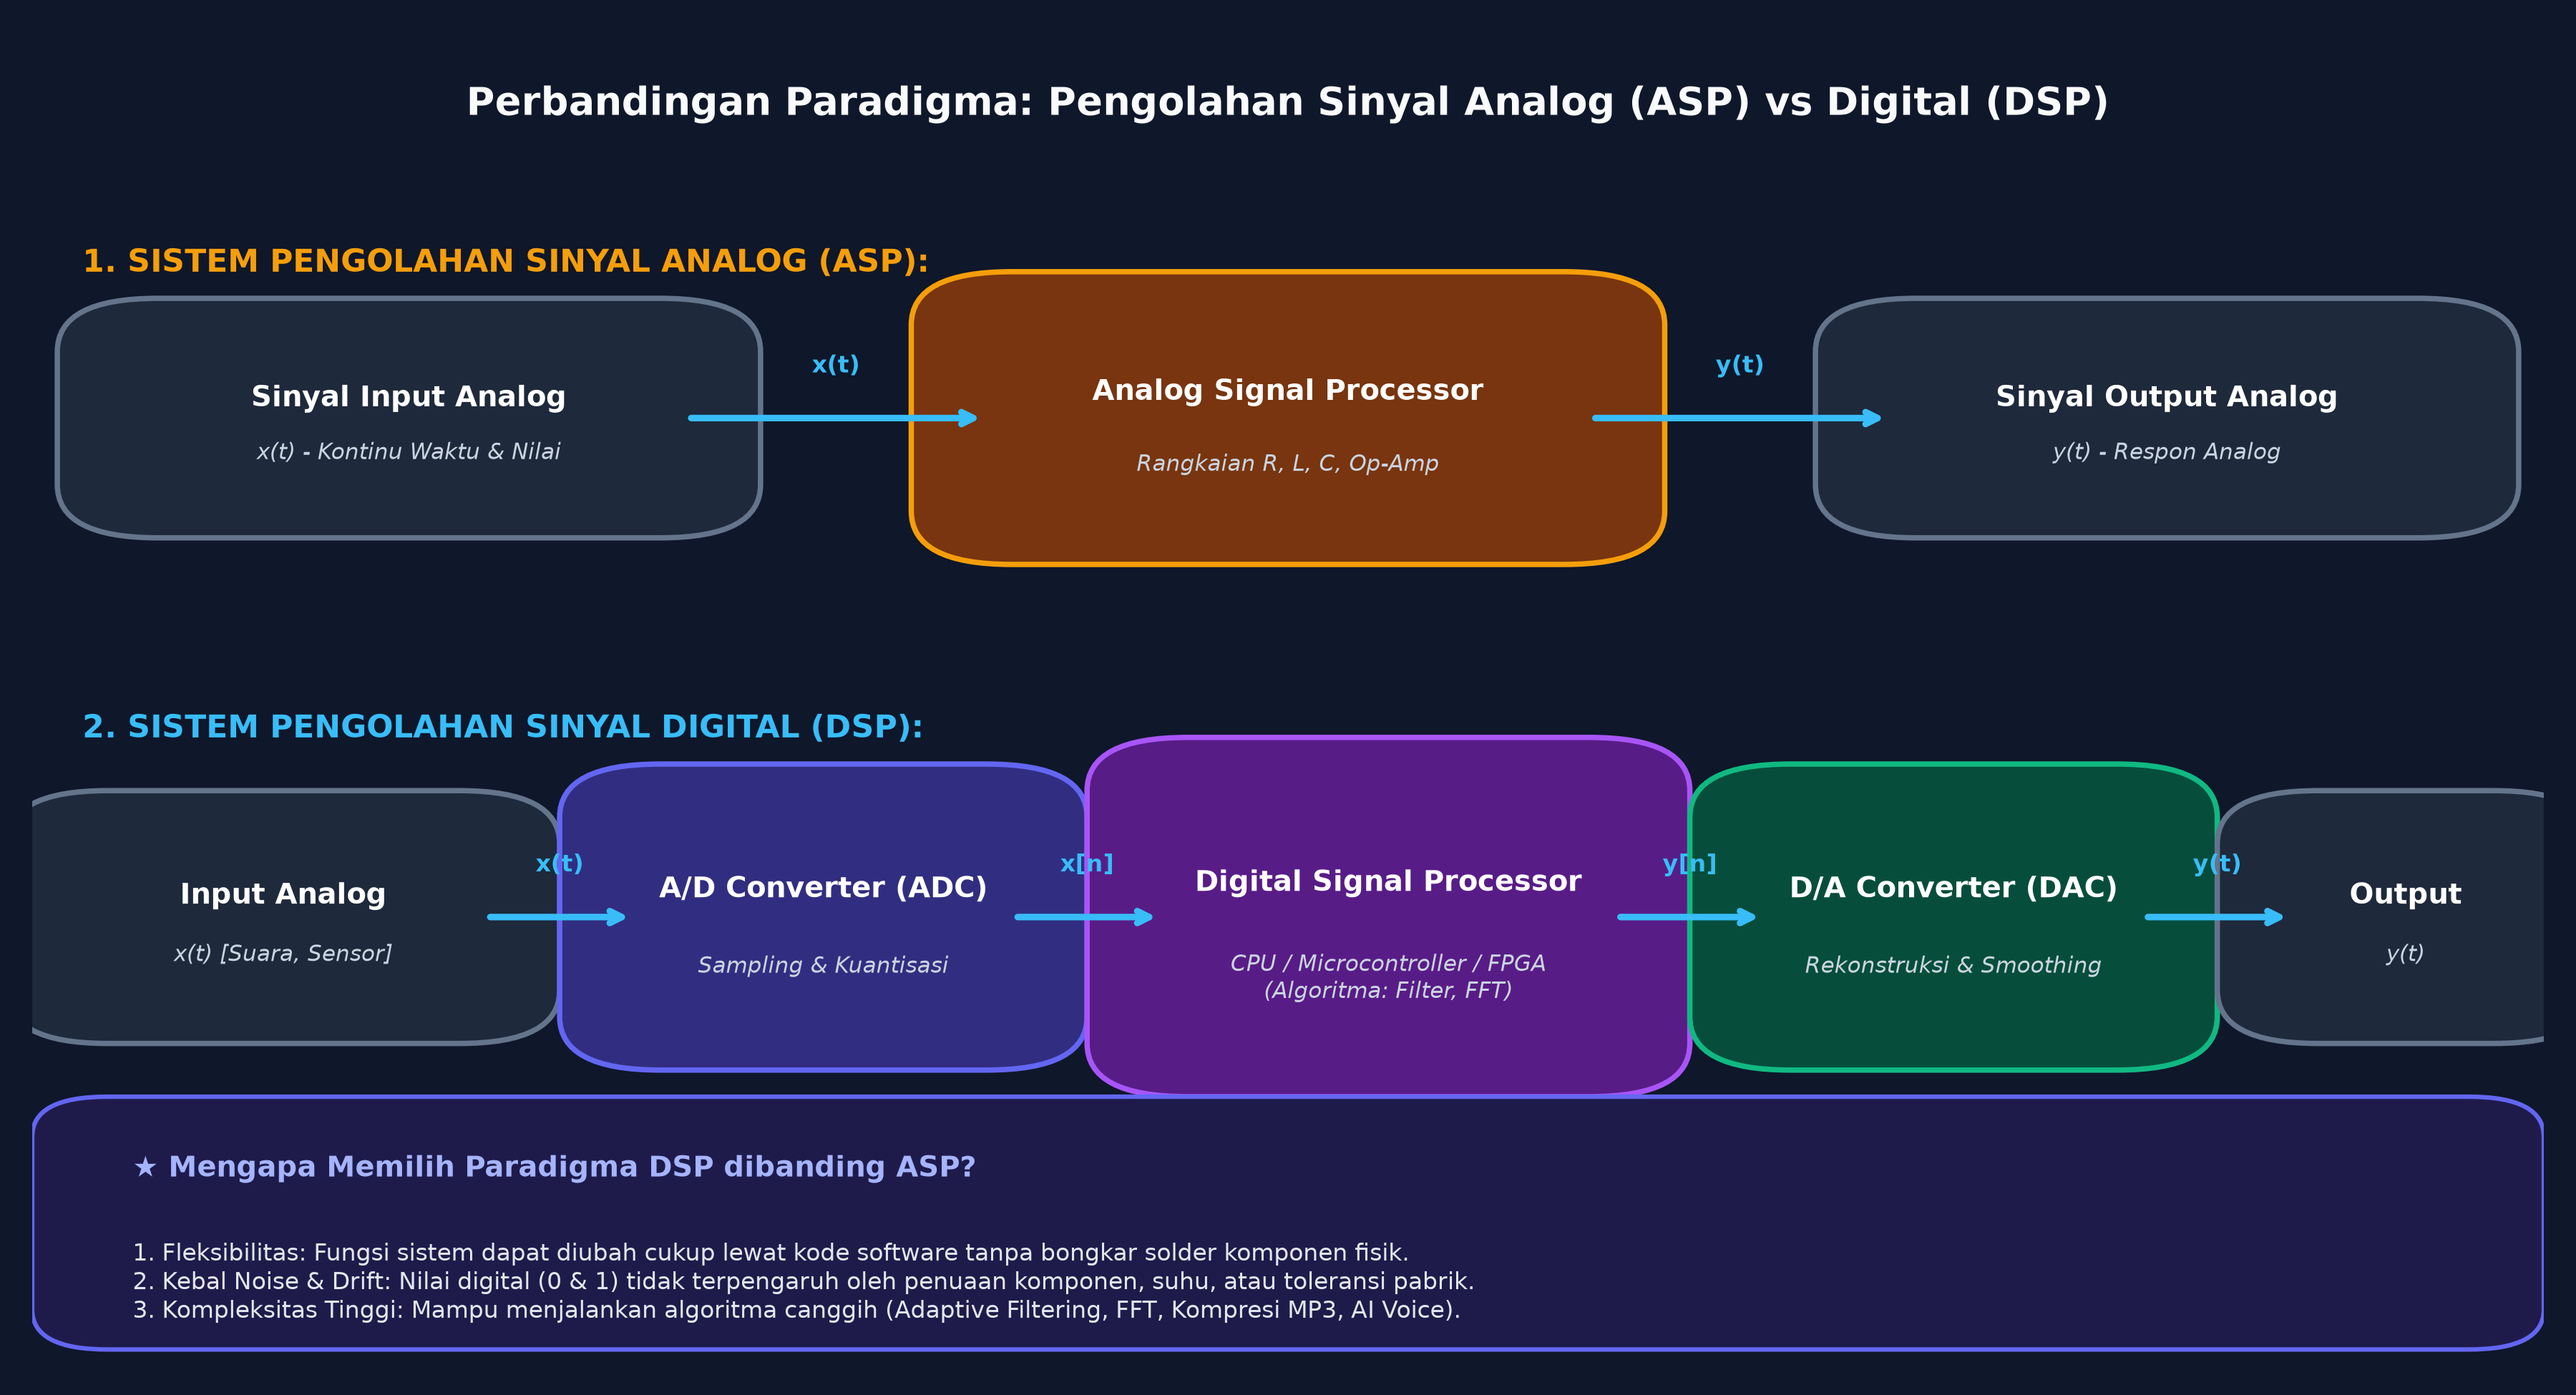
\includegraphics[width=0.92\linewidth]{assets/diagram_asp_vs_dsp.png}
  \captionof{figure}{Komparasi arsitektur perangkat keras: Pemrosesan Sinyal Analog (ASP) vs Pemrosesan Sinyal Digital (DSP).}
\end{center}

\begin{analisisbox}[Formulasi Matematis Sistem ASP vs DSP]
\begin{itemize}[leftmargin=*]
  \item \textbf{Arsitektur Rantai Analog Signal Processing (ASP):}  
  Sistem ASP direalisasikan oleh interkoneksi fisik komponen pasif ($R, L, C$) dan aktif (*Operational Amplifier*). Dinamika sistem kontinu dimodelkan secara rigid oleh Persamaan Diferensial Linier Koefisien Konstan (LCCDE):
  \begin{equation}
  \sum_{k=0}^N a_k \frac{d^k y(t)}{dt^k} = \sum_{m=0}^M b_m \frac{d^m x(t)}{dt^m} \quad \xrightarrow{\mathcal{L}} \quad H(s) = \frac{Y(s)}{X(s)} = \frac{\sum_{m=0}^M b_m s^m}{\sum_{k=0}^N a_k s^k}
  \end{equation}
  \textit{Kelemahan Kritis ASP:} Sensitivitas tinggi terhadap toleransi komponen $\frac{\Delta H(s)}{H(s)} \approx \sum_i S_{p_i}^H \frac{\Delta p_i}{p_i}$, drift termal resistansi $\Delta R(T) = R_0(1 + \alpha \Delta T)$, degradasi penuaan elektrolit kapasitor, rentan terhadap induksi dengung jala-jala $50/60\text{ Hz}$, serta ketidakmungkinan merancang filter dengan fase linear murni.

  \item \textbf{Arsitektur Rantai Digital Signal Processing (DSP):}  
  Sistem DSP memetakan cuplikan terkuantisasi melalui algoritma komputasi pada arsitektur prosesor (CPU, ALU, FPGA, DSP Chip). Dinamikanya diatur oleh Persamaan Beda Linier Koefisien Konstan (LCCDDE):
  \begin{equation}
  \sum_{k=0}^N a_k y[n-k] = \sum_{m=0}^M b_m x[n-m] \quad \xrightarrow{\mathcal{Z}} \quad H(z) = \frac{Y(z)}{X(z)} = \frac{\sum_{m=0}^M b_m z^{-m}}{\sum_{k=0}^N a_k z^{-k}}
  \end{equation}
  \textit{Keunggulan Superior DSP:}
  \begin{enumerate}
    \item \textbf{Akurasi \& Reproduktibilitas 100\%:} Bebas dari drift suhu lingkungan dan toleransi nilai fisik komponen.
    \item \textbf{Fleksibilitas Reconfigurability:} Respons filter dapat diubah secara instan secara adaptif (*Adaptive LMS Filtering*) melalui perangkat lunak tanpa modifikasi sirkuit.
    \item \textbf{Fase Linear Sempurna:} Mampu merealisasikan filter FIR simetris dengan penundaan grup konstan ($\tau_g = -\frac{d\theta(\omega)}{d\omega} = \text{konstan}$), mustahil dicapai pada ASP.
  \end{enumerate}
\end{itemize}
\end{analisisbox}

\vspace{0.3cm}
\subsection{Tiga Pilar Anatomi Gelombang: Amplitudo, Frekuensi, dan Fase}

Persamaan matematis gelombang sinusoidal waktu-kontinu dinyatakan dalam domain riil dan domain kompleks Euler:
\begin{equation}
x(t) = A \sin(2\pi f t + \phi) = A \sin(\Omega t + \phi) \equiv \operatorname{Re}\left\{ A e^{j(\Omega t + \phi)} \right\} = \frac{A}{2j} e^{j(\Omega t + \phi)} - \frac{A}{2j} e^{-j(\Omega t + \phi)}
\end{equation}

\begin{center}
  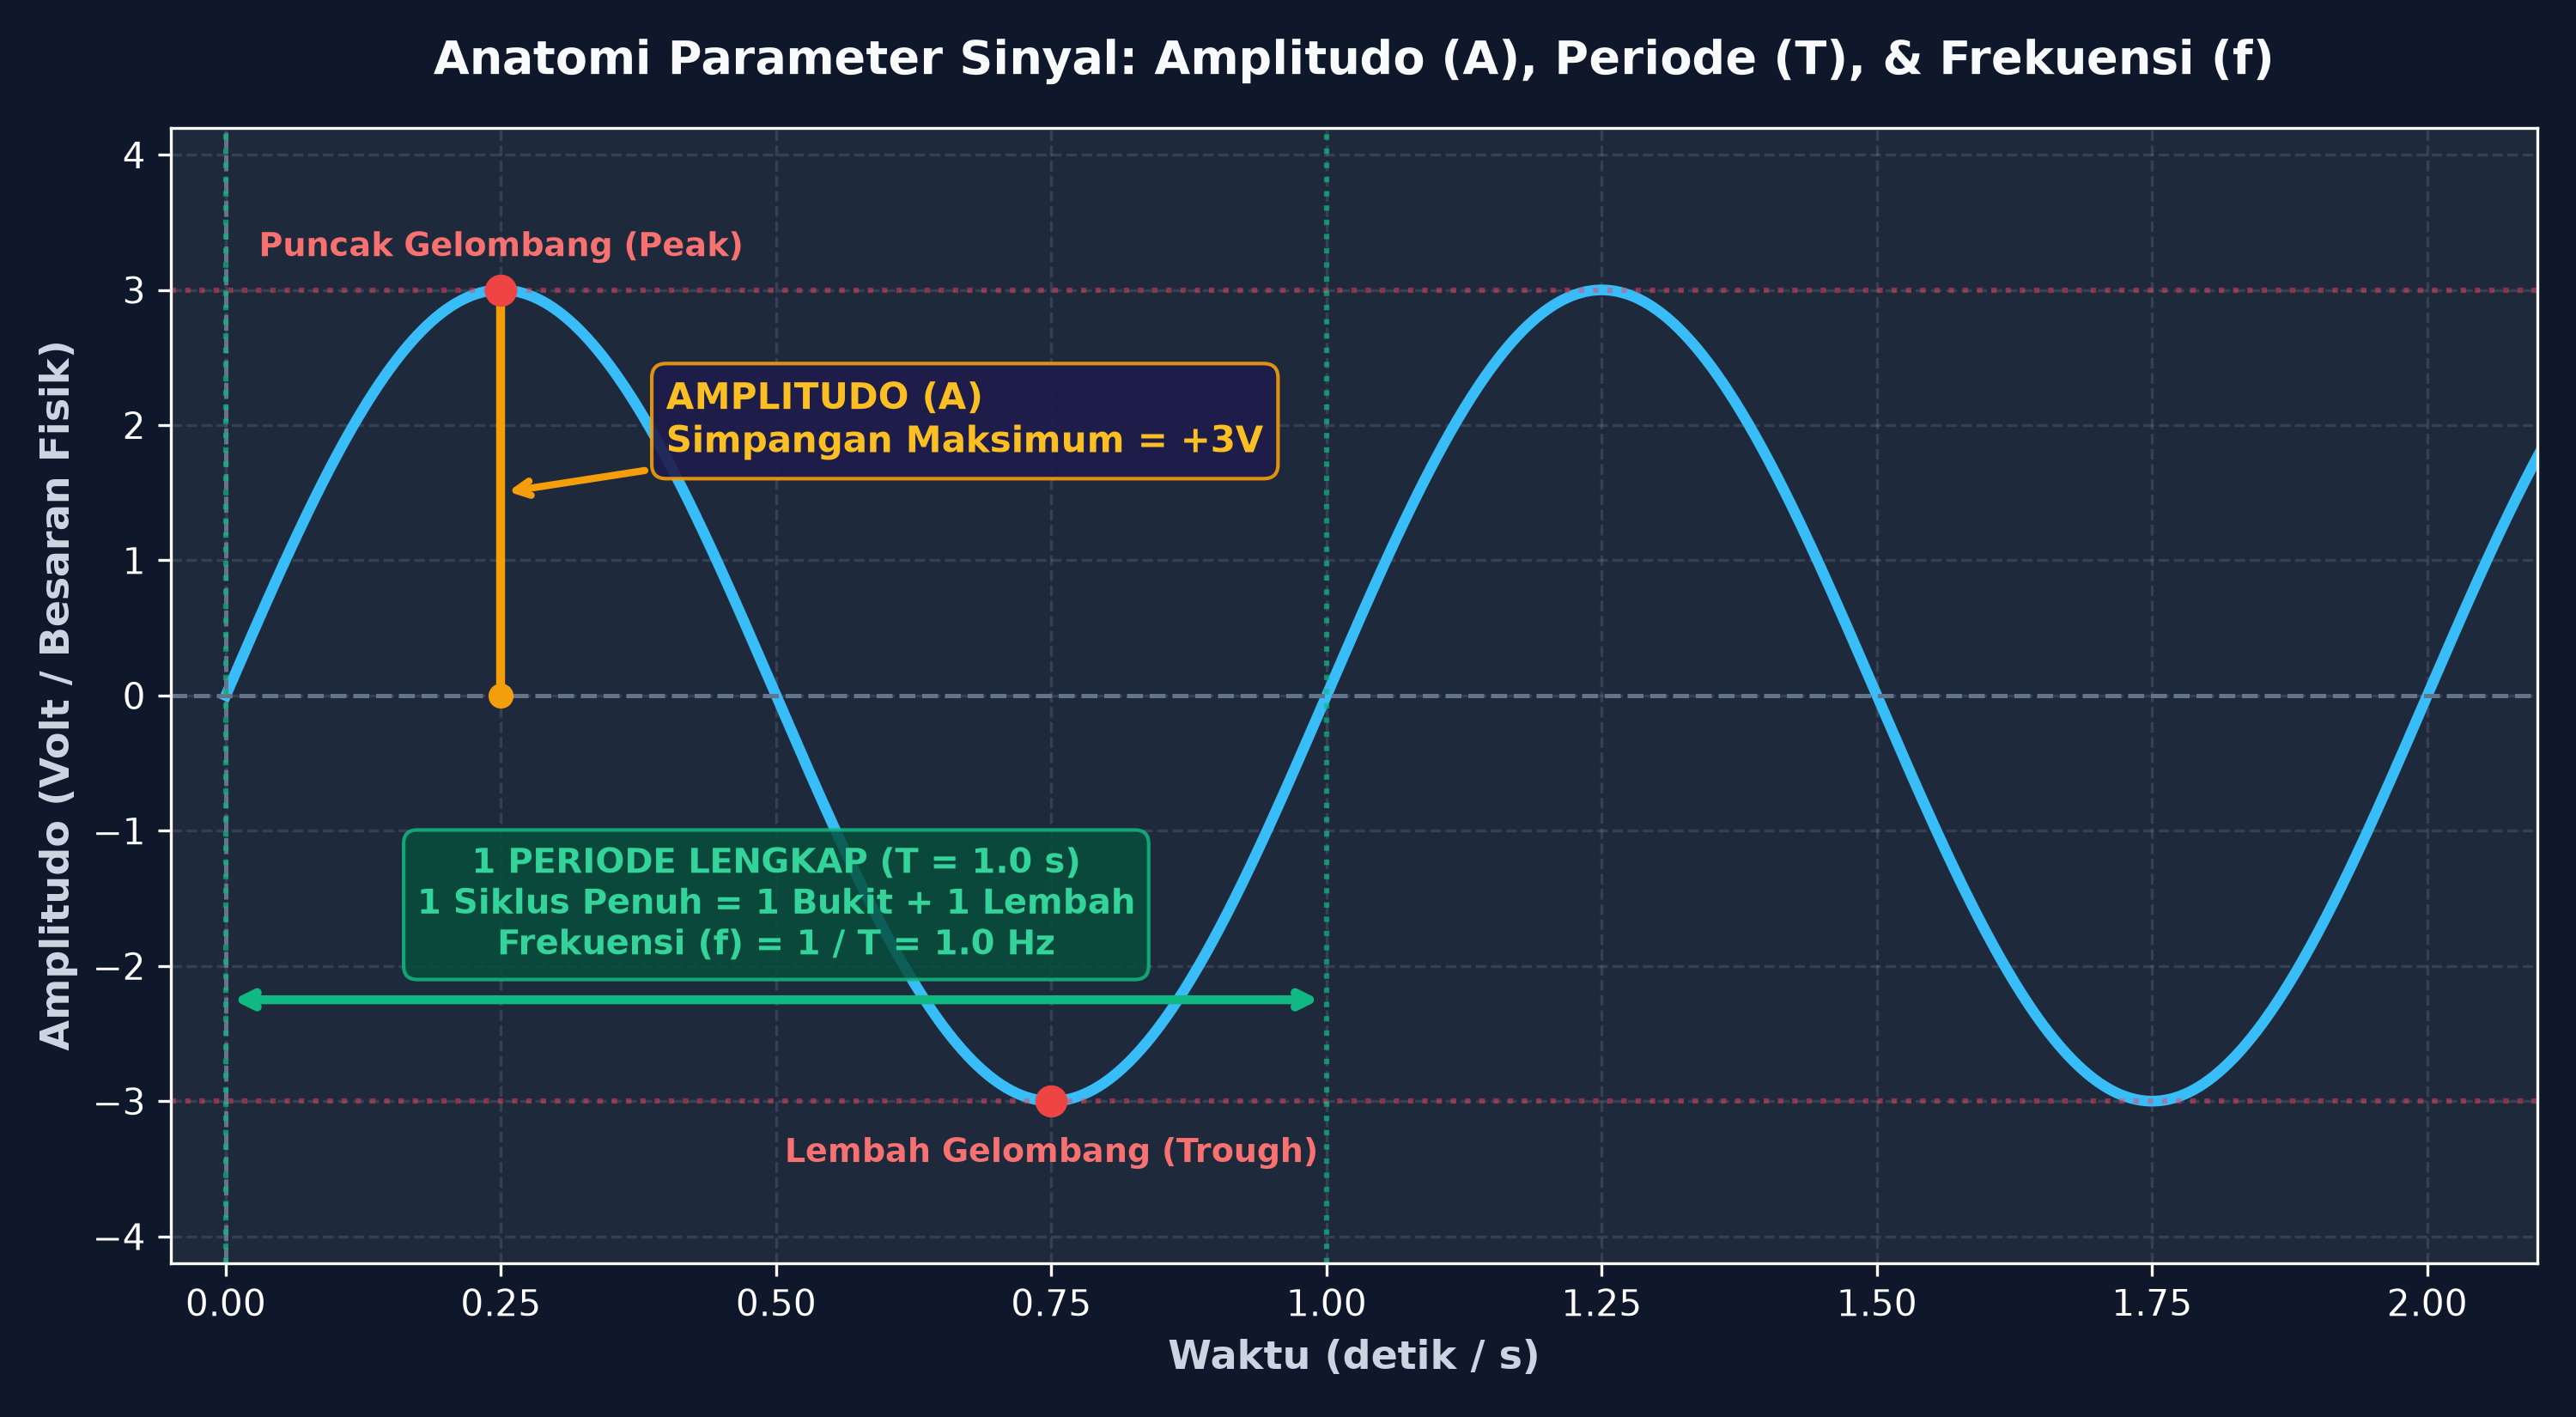
\includegraphics[width=0.85\linewidth]{assets/anatomi_sinyal.png}
  \captionof{figure}{Anatomi geometris sinyal sinusoidal kontinu: Amplitudo Puncak ($A$), Nilai Peak-to-Peak ($V_{\text{pp}} = 2A$), Periode Fundamental ($T$), dan Pergeseran Fase ($\phi$).}
\end{center}

\begin{center}
  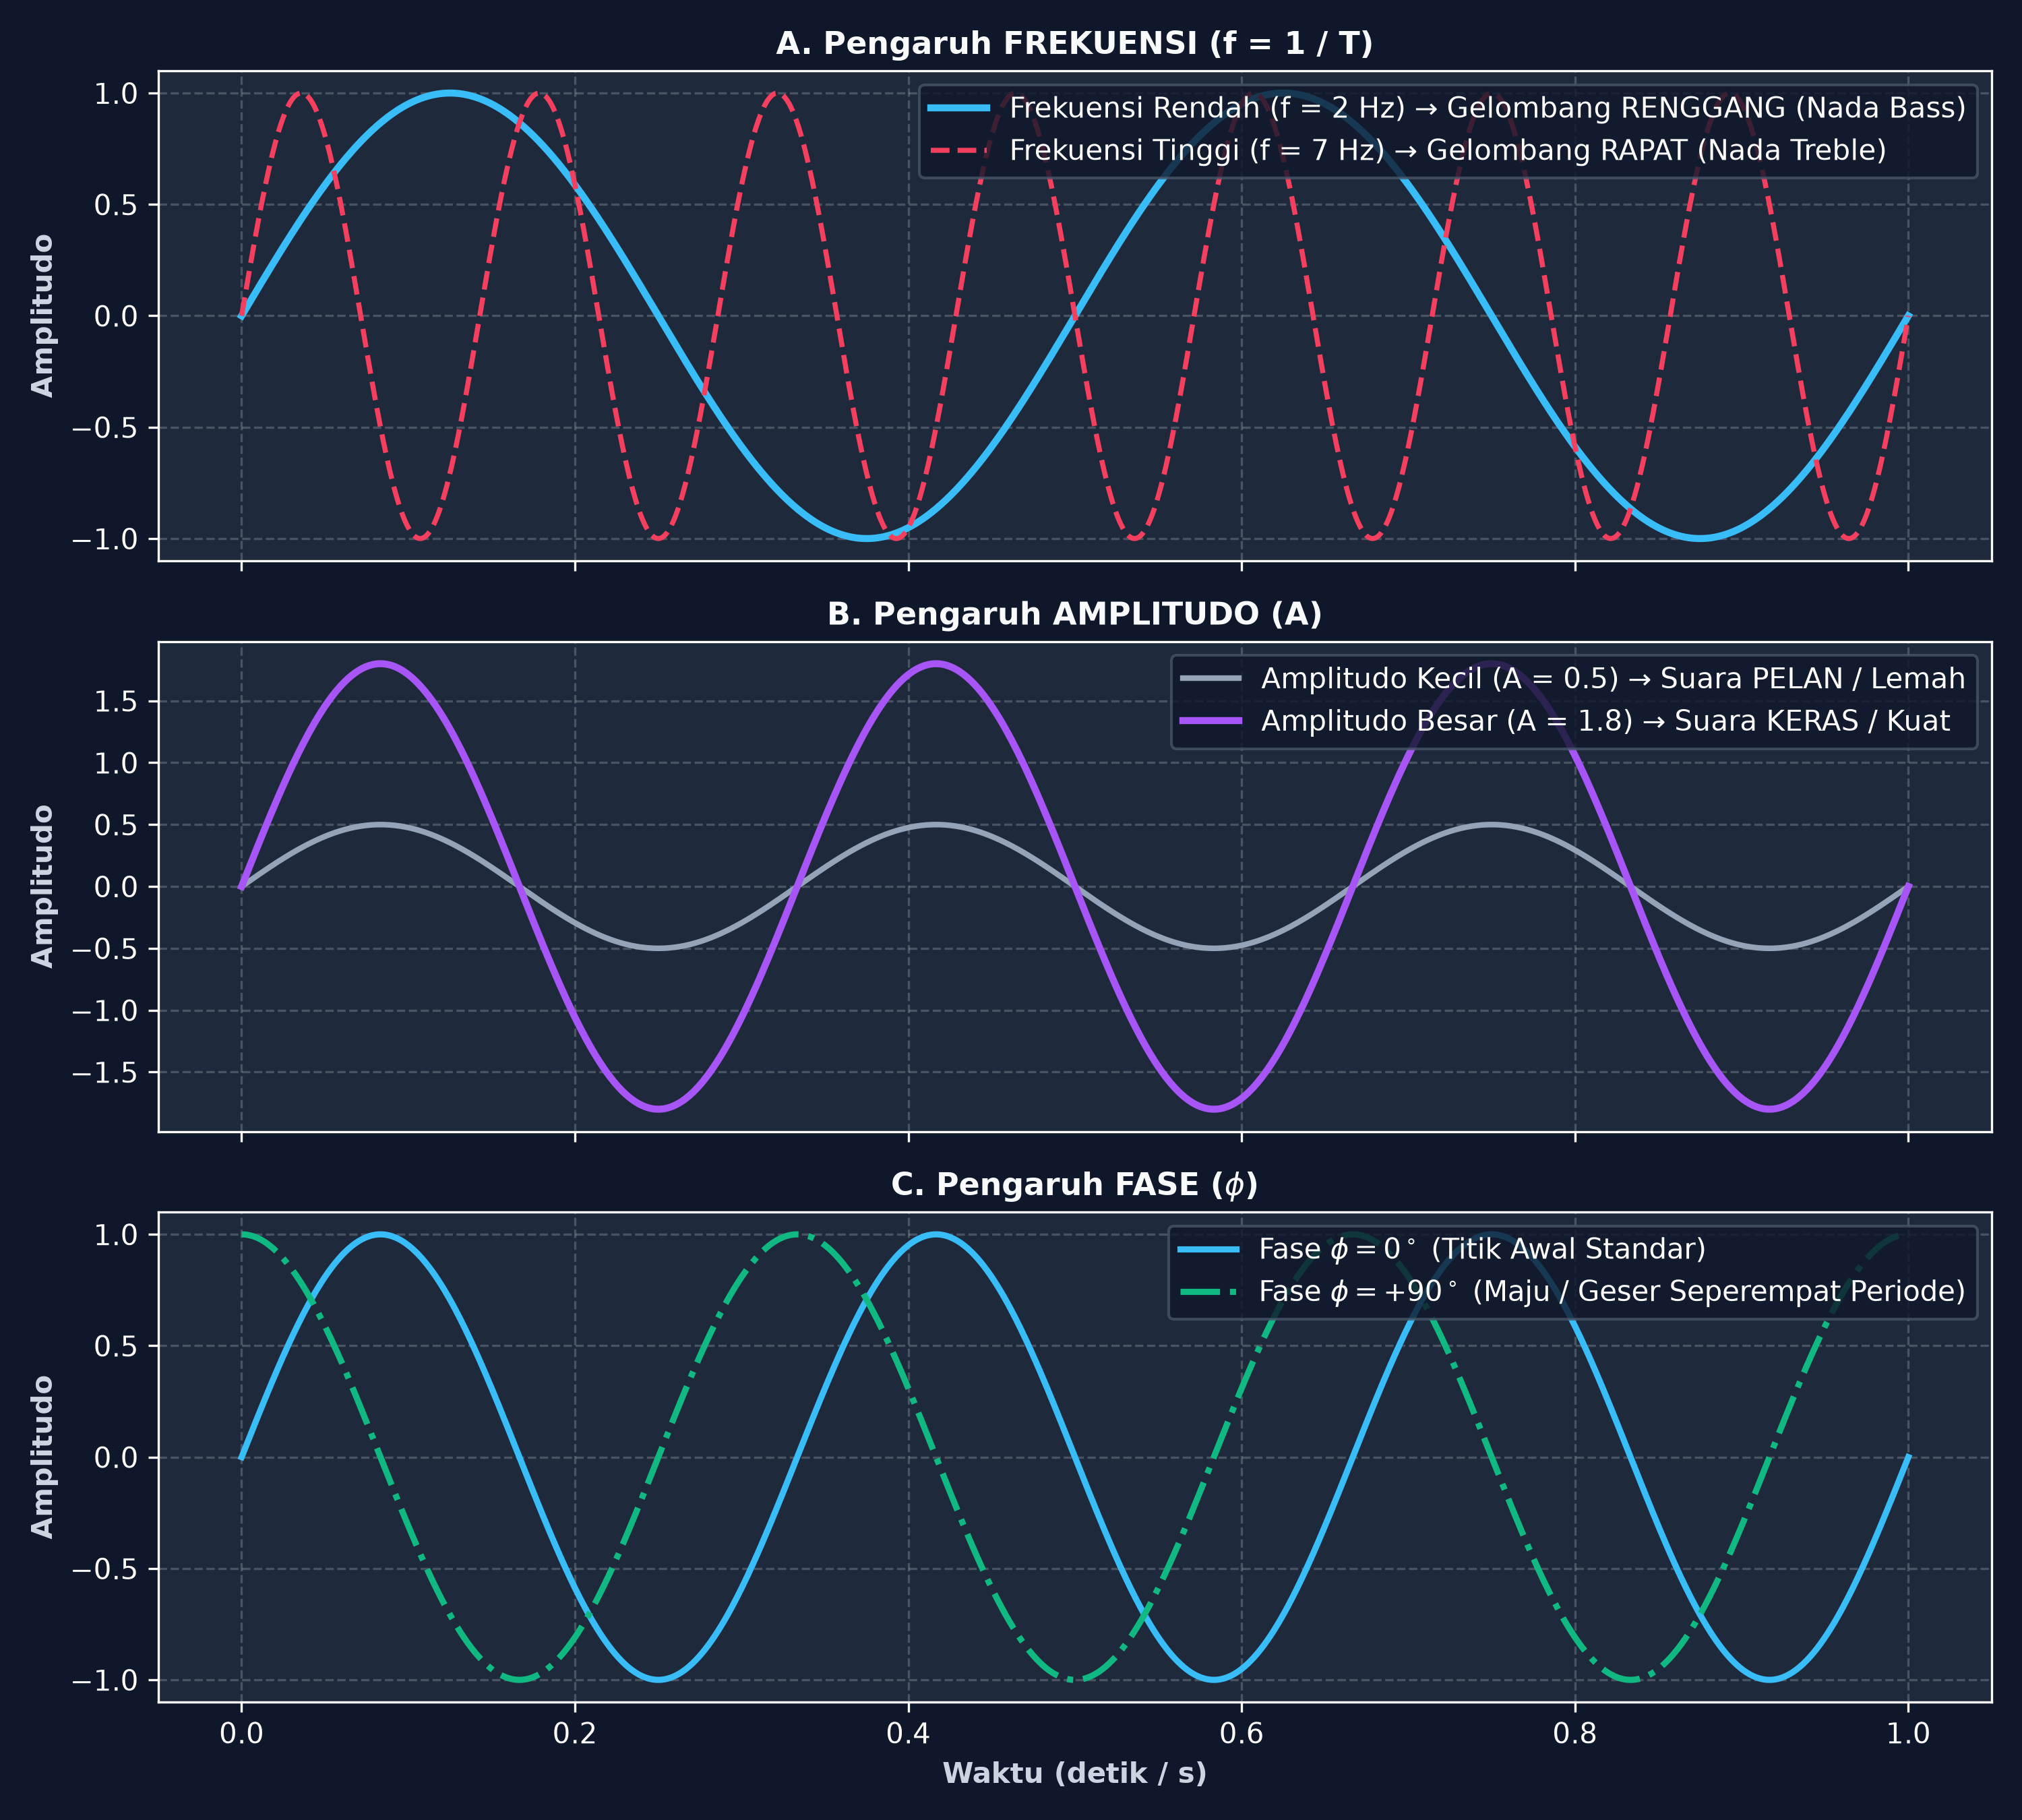
\includegraphics[width=0.92\linewidth]{assets/komparasi_sinyal.png}
  \captionof{figure}{Efek ortogonal pemisahan parameter gelombang: Modulasi Frekuensi (Panel 1), Modulasi Amplitudo (Panel 2), dan Modulasi Fase Kuadratur (Panel 3).}
\end{center}

\begin{analisisbox}[Karakterisasi Energi \& Parameter Gelombang]
\begin{enumerate}[leftmargin=*]
  \item \textbf{Amplitudo ($A$) \& Daya Sinyal ($P_{\text{avg}}$):}  
  Menentukan besaran simpangan puncak dari titik keseimbangan. Nilai kuadrat rata-rata (*Root-Mean-Square* / RMS) dan daya rata-rata untuk gelombang sinus beban $1\ \Omega$ adalah:
  \begin{equation}
  V_{\text{rms}} = \sqrt{\frac{1}{T}\int_0^T x^2(t) dt} = \frac{A}{\sqrt{2}}, \qquad P_{\text{avg}} = V_{\text{rms}}^2 = \frac{A^2}{2}
  \end{equation}
  
  \item \textbf{Frekuensi Siklik ($f$), Sudut ($\Omega$), dan Periode ($T$):}  
  $f$ mengukur laju osilasi per satuan waktu (Hertz $\equiv \text{s}^{-1}$), $\Omega = 2\pi f$ adalah kecepatan sudut ($\text{rad/s}$), dan periode fundamental $T = \frac{1}{f} = \frac{2\pi}{\Omega}$. Pada Gambar Komparasi Panel 1, peningkatan frekuensi dari $1\text{ Hz}$ ke $3\text{ Hz}$ melipatgandakan kerapatan energi spektral pada sumbu frekuensi.

  \item \textbf{Fase Awal ($\phi$) \& Pergeseran Waktu ($\Delta t$):}  
  Pergeseran fase $\phi$ setara secara eksak dengan translasi waktu $\Delta t = -\frac{\phi}{\Omega} = -\frac{\phi}{2\pi f}$. Jika $\phi = +90^\circ = +\frac{\pi}{2}\text{ rad}$ (Gambar Komparasi Panel 3), gelombang bertransformasi menjadi fungsi cosinus:
  \begin{equation}
  x(t) = A \sin\left(\Omega t + \frac{\pi}{2}\right) = A \cos(\Omega t)
  \end{equation}
  yang mengindikasikan komponen kuadratur ($Q$-channel) mendahului (*leading*) komponen in-phase ($I$-channel) sebesar $\Delta t = -T/4$.
\end{enumerate}
\end{analisisbox}

\newpage
\subsection{Sistem Pengolah Sinyal \& 4 Klasifikasi Karakteristik Operasinya}

Suatu sistem waktu-diskrit didefinisikan sebagai transformasi matematis atau operator $\mathcal{T}\{\cdot\}$ yang memetakan sinyal masukan $x[n]$ menjadi sinyal keluaran $y[n] = \mathcal{T}\{x[n]\}$.

\begin{center}
  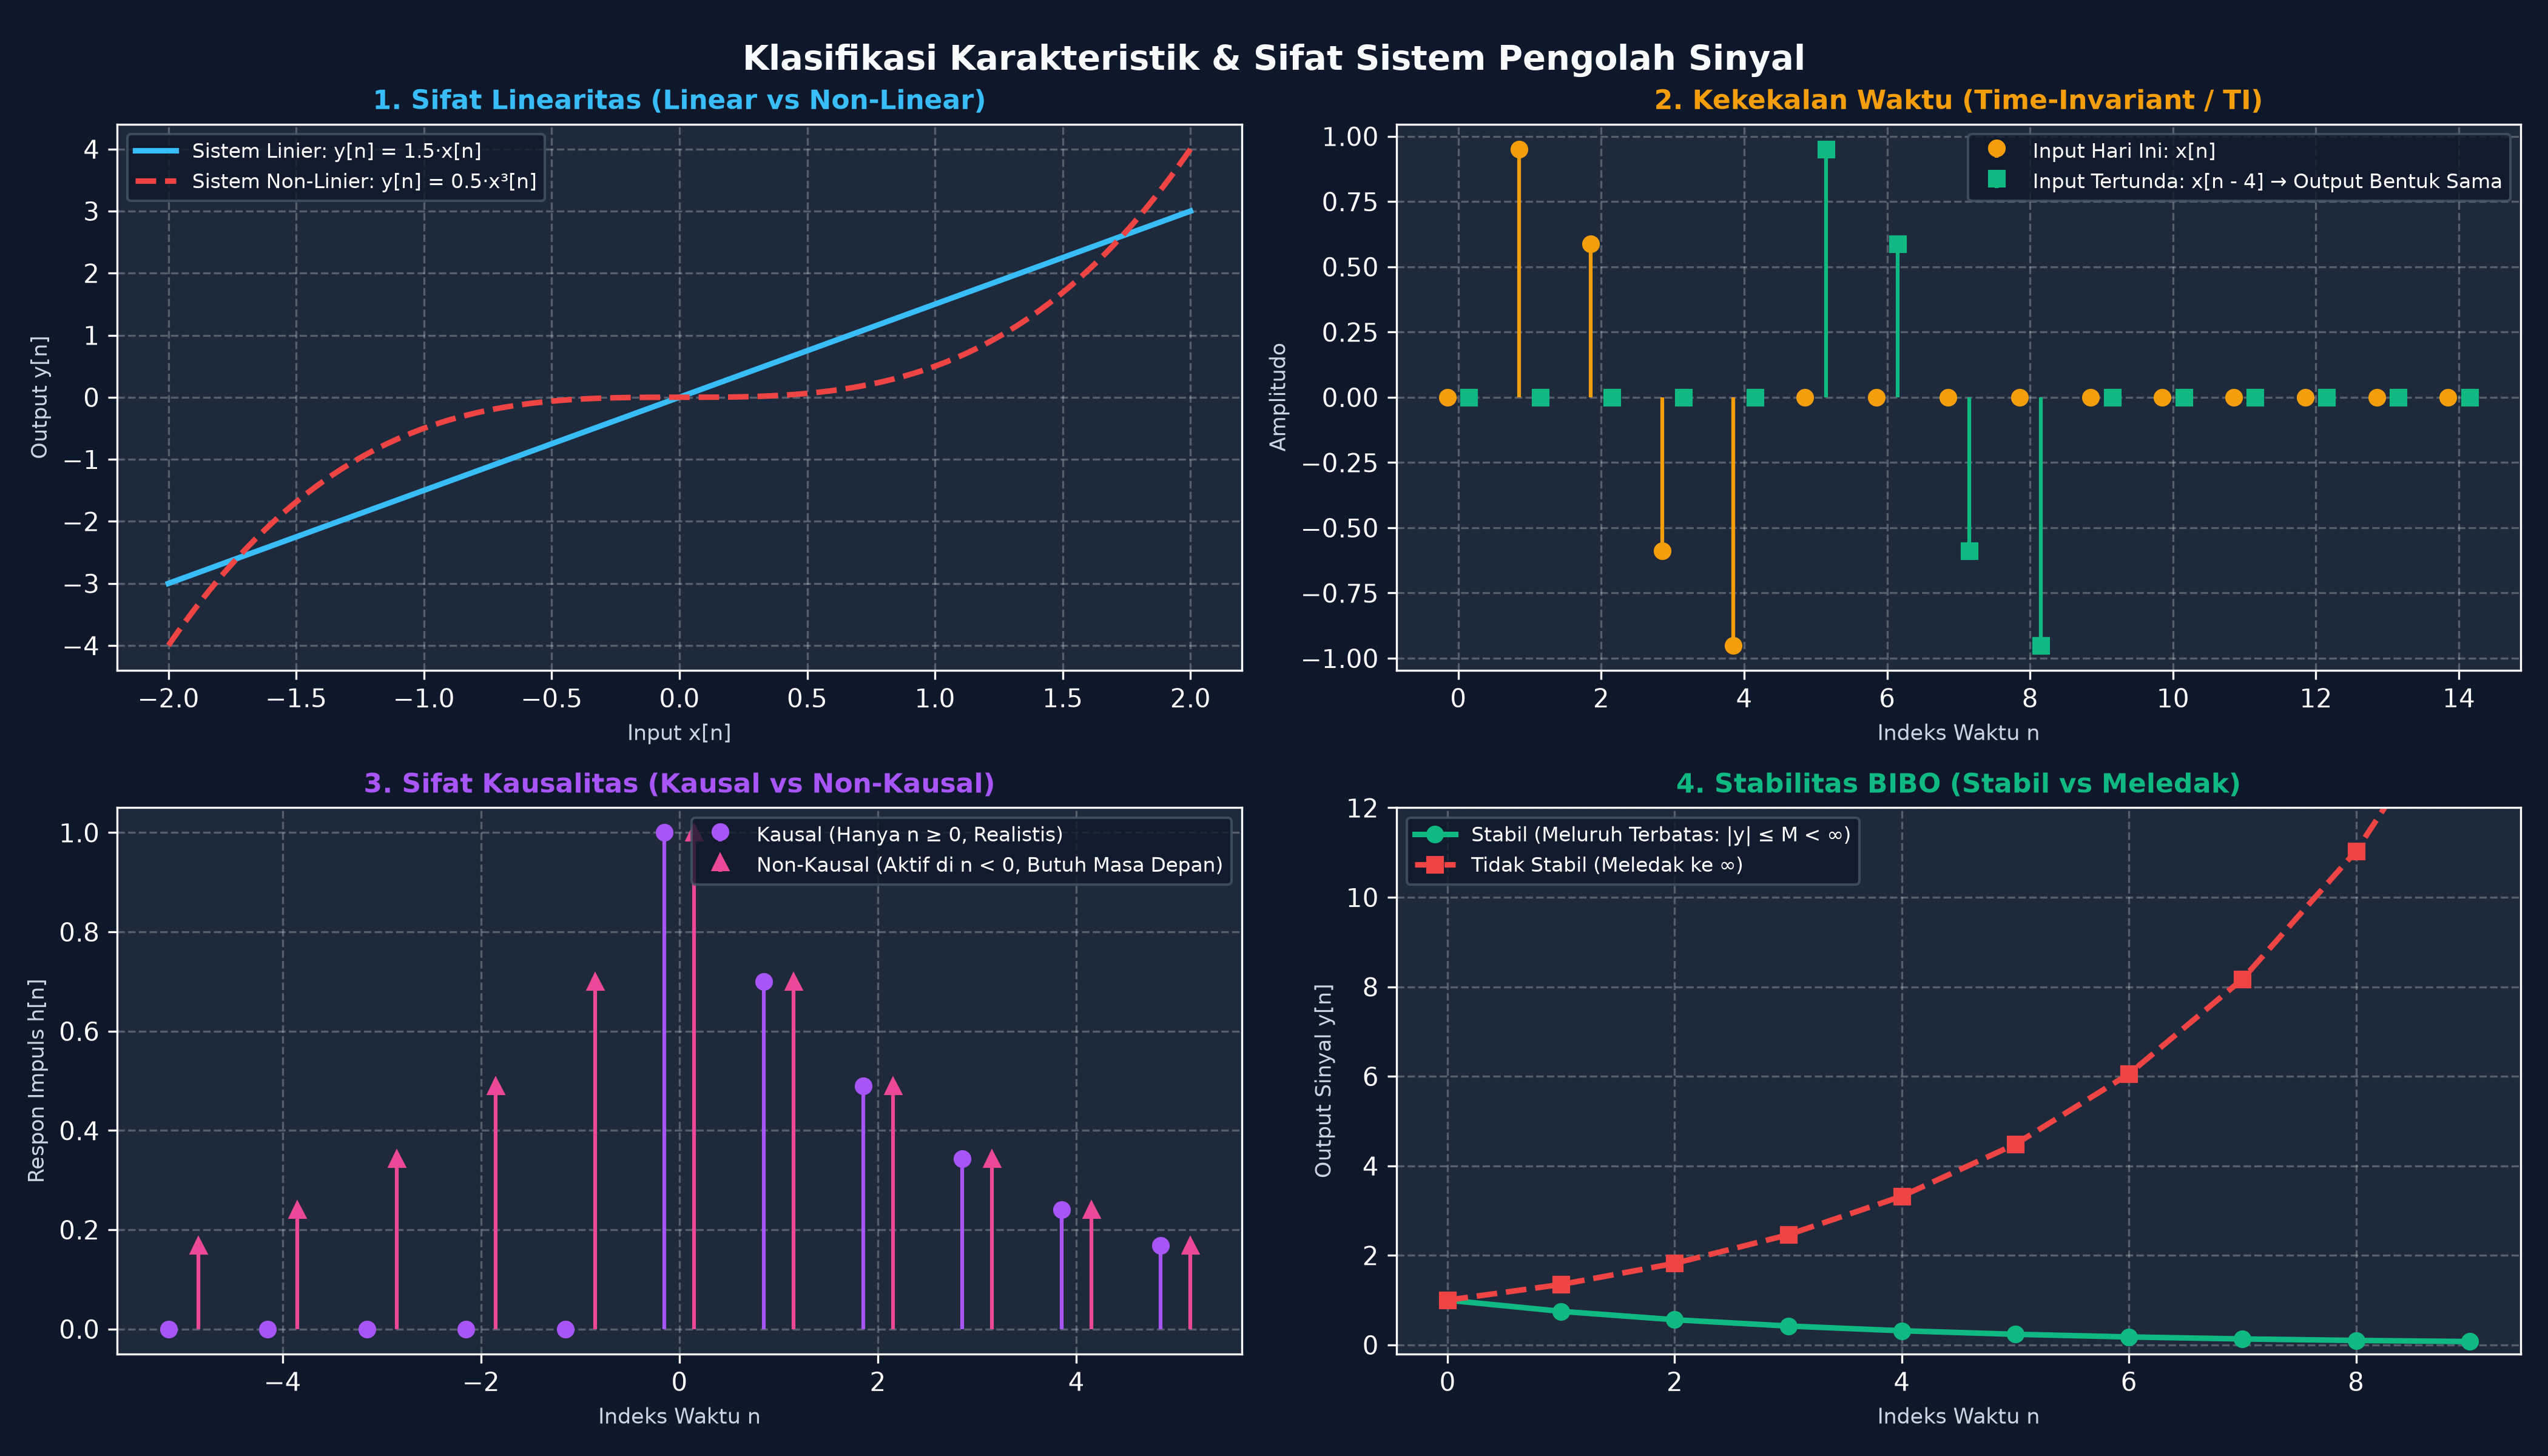
\includegraphics[width=0.95\linewidth]{assets/klasifikasi_sistem.png}
  \captionof{figure}{Empat pilar klasifikasi sistem: (1) Linearitas, (2) Time-Invariance, (3) Kausalitas, dan (4) Stabilitas BIBO.}
\end{center}

\begin{analisisbox}[Uji Matematis Rigor Empat Sifat Karakteristik Sistem]
\begin{enumerate}[leftmargin=*]
  \item \textbf{Linearitas (Superposisi \& Homogenitas):}  
  Sistem linier wajib memenuhi prinsip superposisi simultan:
  \begin{equation}
  \mathcal{T}\left\{ \alpha x_1[n] + \beta x_2[n] \right\} = \alpha \mathcal{T}\{x_1[n]\} + \beta \mathcal{T}\{x_2[n]\} = \alpha y_1[n] + \beta y_2[n], \quad \forall \alpha, \beta \in \mathbb{C}
  \end{equation}
  \textit{Analisis Visual (Panel 1):} Sistem $y[n] = 1.5 x[n]$ membentuk garis linier proporsional sempurna. Sebaliknya, sistem kubik $y[n] = 0.5 x^3[n]$ bersifat non-linier; jika dimasukkan input harmonisa tunggal $x[n] = \cos(\omega_0 n)$, keluarannya menghasilkan distorsi harmonisa ganjil $\cos^3(\omega_0 n) = \frac{3}{4}\cos(\omega_0 n) + \frac{1}{4}\cos(3\omega_0 n)$, memunculkan komponen frekuensi baru $3\omega_0$ yang merusak integritas sinyal asli.

  \item \textbf{Kekekalan Waktu (Time-Invariance / TI):}  
  Operator sistem komutatif terhadap operator pergeseran waktu $\mathcal{S}_{n_0}\{x[n]\} = x[n - n_0]$:
  \begin{equation}
  \mathcal{T}\left\{ \mathcal{S}_{n_0}\{x[n]\} \right\} = \mathcal{S}_{n_0}\left\{ \mathcal{T}\{x[n]\} \right\} \iff \mathcal{T}\{x[n - n_0]\} = y[n - n_0]
  \end{equation}
  \textit{Analisis Visual (Panel 2):} Input yang ditunda sejauh $n_0 = 4$ detik menghasilkan kurva hijau yang identik secara morfologi dengan kurva oranye tanpa distorsi bentuk.

  \item \textbf{Kausalitas (Causality):}  
  Keluaran sistem pada setiap indeks $n = n_0$ hanya bergantung pada nilai masukan saat ini dan masa lalu ($x[n]$ untuk $n \leq n_0$). Syarat perlu dan cukup untuk sistem Linier Time-Invariant (LTI) kausal adalah respon impulsnya harus nol untuk indeks waktu negatif:
  \begin{equation}
  h[n] = 0, \quad \forall n < 0
  \end{equation}
  \textit{Analisis Visual (Panel 3):} Respon ungu ($h[n] \neq 0$ hanya saat $n \geq 0$) bersifat kausal (*realizable* di dunia nyata). Respon pink aktif saat $n < 0$, mengindikasikan sistem non-kausal yang memerlukan pengetahuan input masa depan.

  \item \textbf{Stabilitas BIBO (Bounded-Input Bounded-Output):}  
  Sistem stabil BIBO menjamin bahwa untuk setiap masukan terbatas $|x[n]| \leq M_x < \infty, \forall n$, keluarannya terikat terbatas $|y[n]| \leq M_y < \infty, \forall n$. Syarat perlu dan cukup untuk sistem LTI stabil BIBO adalah respon impulsnya \textbf{terjumlahkan secara mutlak} (*absolutely summable*):
  \begin{equation}
  S_h = \sum_{k=-\infty}^{\infty} |h[k]| < \infty
  \end{equation}
  \textit{Analisis Visual (Panel 4):} Untuk sistem orde-1 dengan respon impuls $h[n] = a^n u[n]$:
  \[
  S_h = \sum_{n=0}^{\infty} |a|^n = \frac{1}{1 - |a|} \quad \text{konvergen jika dan hanya jika } |a| < 1
  \]
  Kurva hijau ($a = 0.75 < 1$) menghasilkan $S_h = \frac{1}{1 - 0.75} = 4 < \infty$ (Stabil). Kurva merah ($a = 1.35 > 1$) menghasilkan deret divergen $S_h \to \infty$, memicu osilasi tak hingga yang merusak rangkaian (*Unstable*).
\end{enumerate}
\end{analisisbox}

\newpage
% =========================================================================
\section{Proses Digitalisasi Sinyal (Analog-to-Digital Converter / ADC)}
% =========================================================================

\subsection{Rantai 4 Tahap Lengkap Digitalisasi ADC}

Konversi sinyal analog kontinu menjadi kata biner digital melibatkan empat tahapan fisika-matematis yang terdefinisi secara ketat:

\begin{center}
  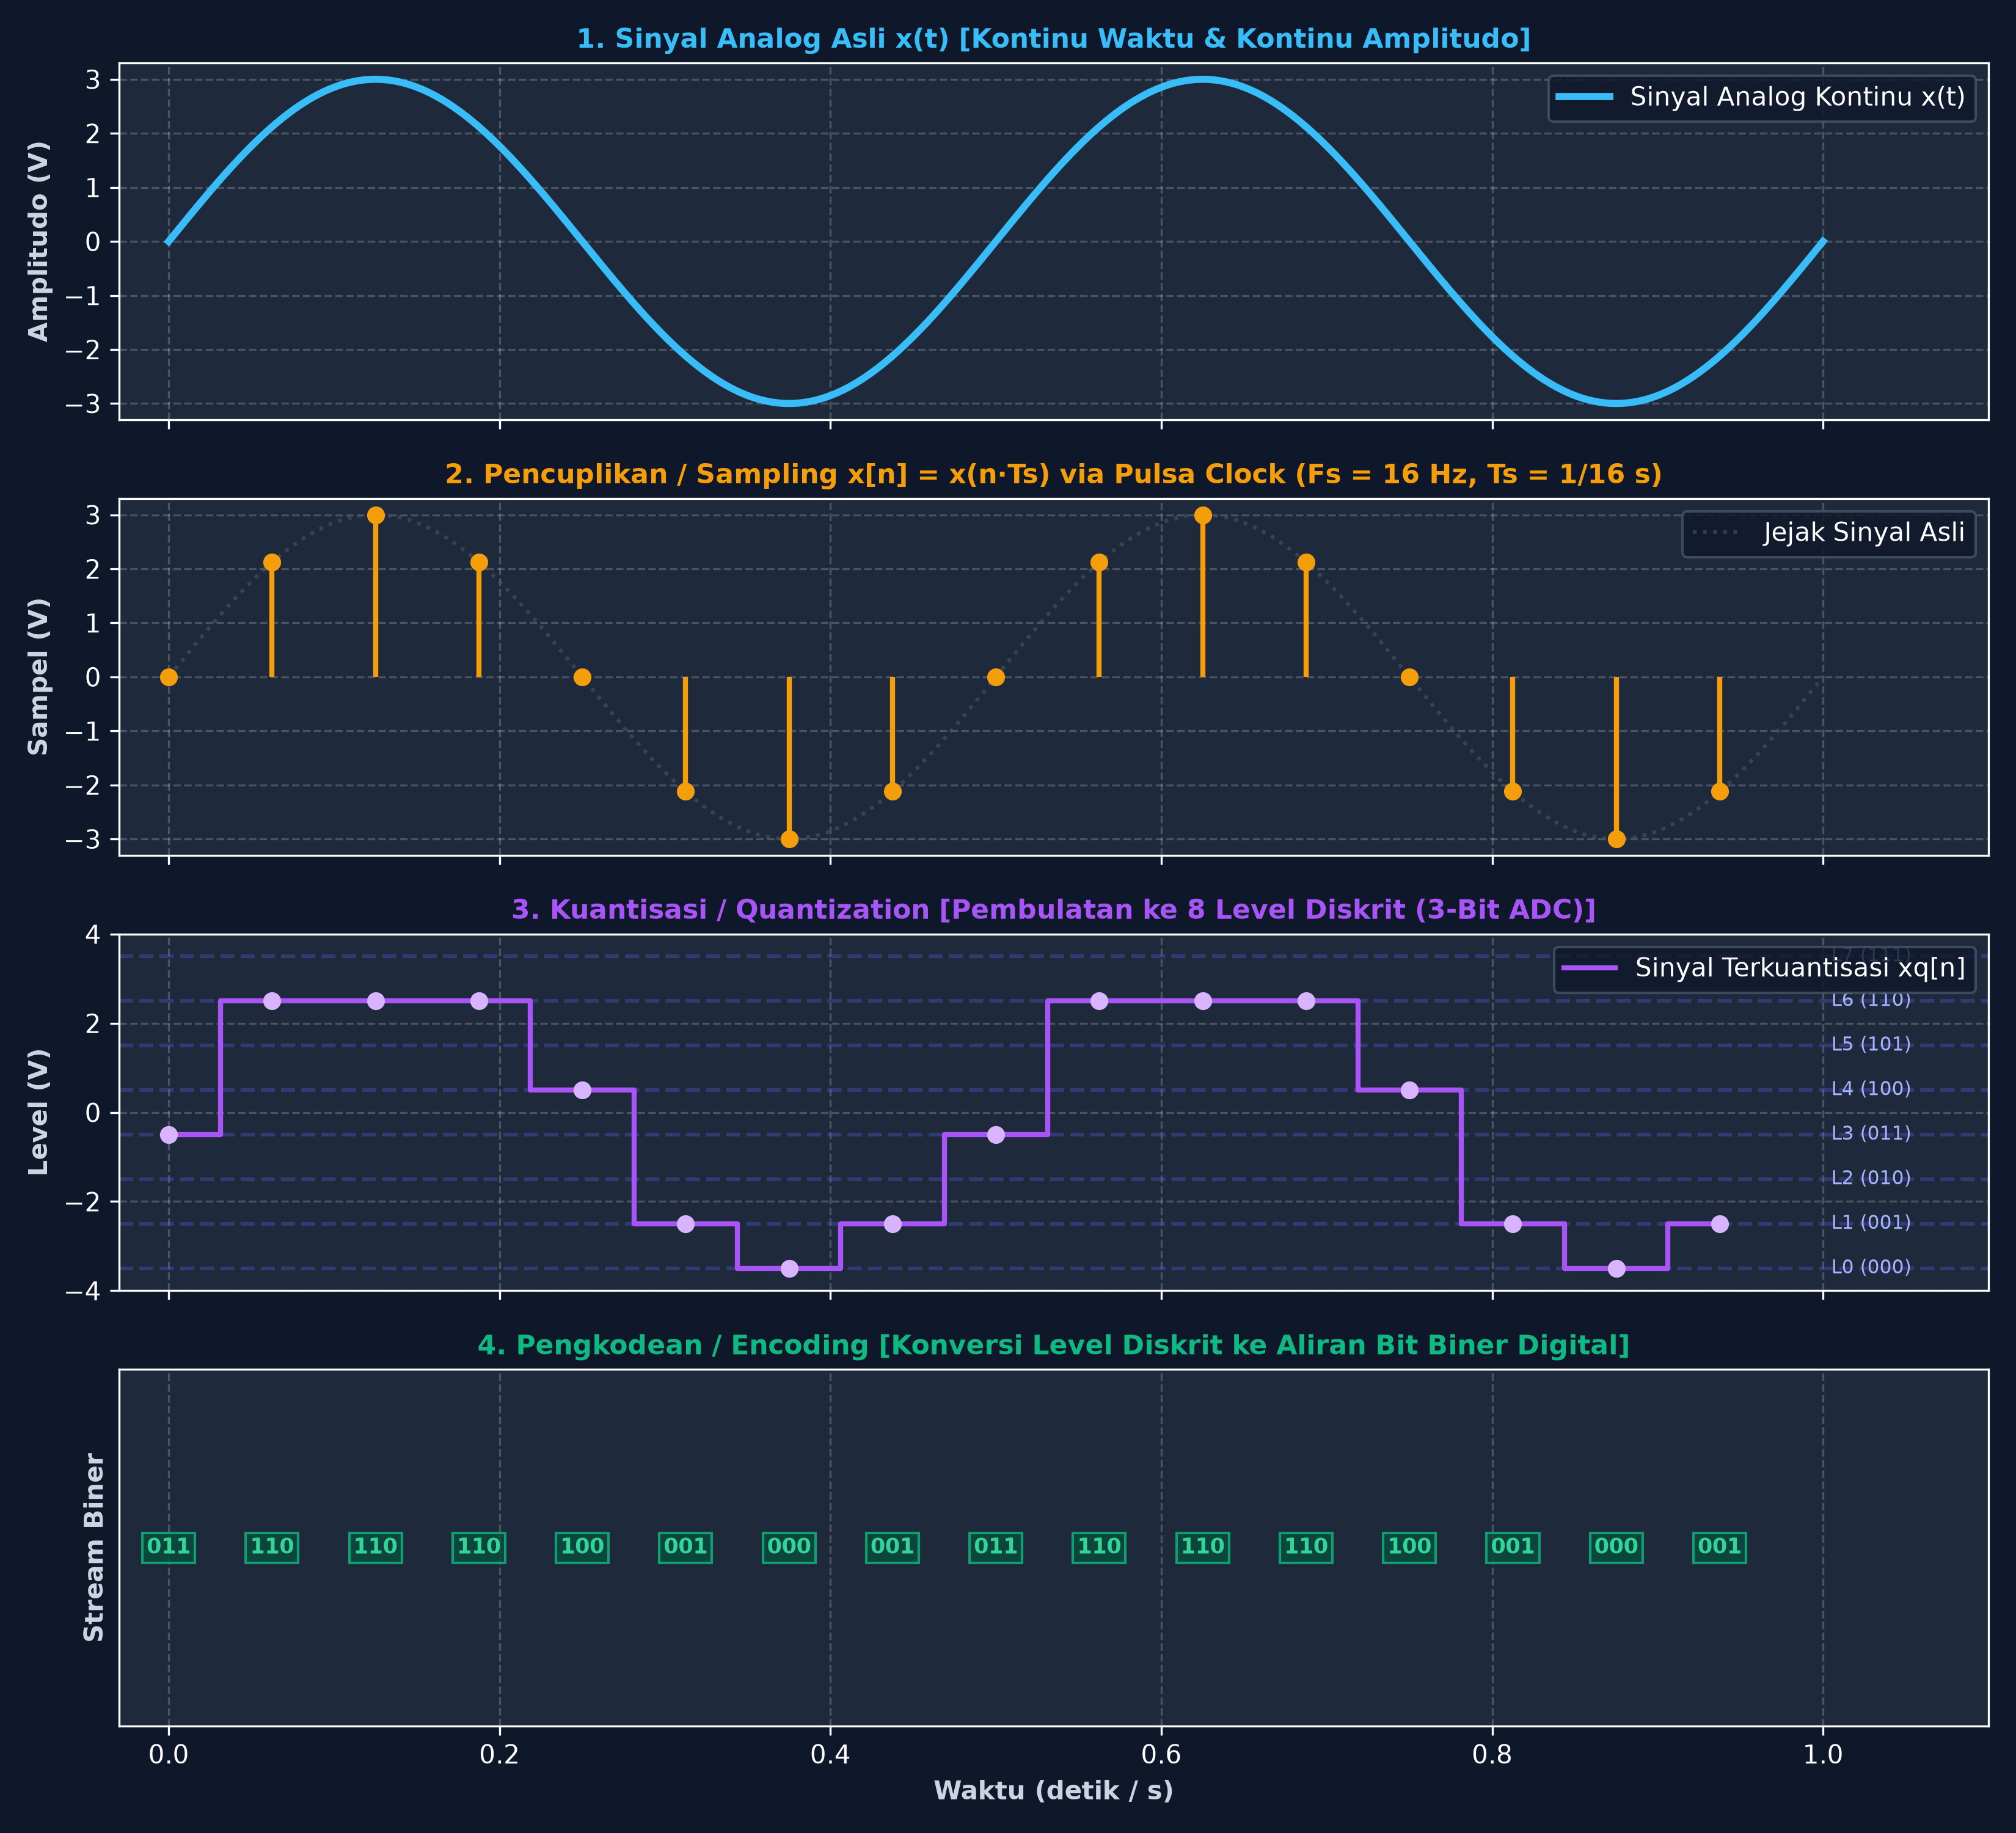
\includegraphics[width=0.95\linewidth]{assets/tahapan_adc_sampling_kuantisasi.png}
  \captionof{figure}{Empat tahapan lengkap digitalisasi ADC: (1) Sinyal Analog Asli, (2) Pencuplikan Diskrit Waktu, (3) Kuantisasi Amplitudo Diskrit, dan (4) Pengkodean Biner.}
\end{center}

\begin{analisisbox}[Formulasi Matematis 4 Blok Digitalisasi ADC]
\begin{enumerate}[leftmargin=*]
  \item \textbf{Anti-Aliasing Filter (AAF) \& Sinyal Asli $x_a(t)$:}  
  Sinyal input analog kontinu $x_a(t) \in \mathbb{R}$ dilewatkan ke filter lolos-rendah (*low-pass filter*) analog dengan frekuensi cut-off $f_c \leq F_s / 2$ untuk memangkas komponen frekuensi tinggi di atas batas Nyquist.

  \item \textbf{Pencuplikan Ideal (Ideal Impulse Train Sampling):}  
  Sinyal dikalikan dengan deretan pulsa Dirac periodik (*Dirac Comb*) $p(t) = \sum_{n=-\infty}^\infty \delta(t - n T_s)$:
  \begin{equation}
  x_s(t) = x_a(t) \cdot p(t) = \sum_{n=-\infty}^\infty x_a(n T_s) \delta(t - n T_s)
  \end{equation}
  Domain waktu menghasilkan deret diskrit $x[n] \equiv x_a(n T_s)$, di mana waktu kini terdiskritisasi menjadi bilangan bulat $n \in \mathbb{Z}$, namun nilai amplitudo $x[n] \in \mathbb{R}$ masih berkesinambungan kontinu (*infinite precision*).

  \item \textbf{Kuantisasi Amplitudo Non-Linier ($\mathcal{Q}\{\cdot\}$):}  
  Pemetaan fungsi tangga non-linier $\mathcal{Q}: \mathbb{R} \to \{V_1, V_2, \dots, V_L\}$ membulatkan nilai amplitudo riil $x[n]$ ke level representasi terdekat:
  \begin{equation}
  x_q[n] = \mathcal{Q}\{x[n]\} = x[n] + e_q[n]
  \end{equation}
  di mana $e_q[n] = x_q[n] - x[n]$ adalah galat kuantisasi (*quantization error*). Sinyal kini diskrit dalam waktu dan diskrit dalam nilai amplitudo.

  \item \textbf{Pengkodean Biner (Binary Word Encoding $\mathcal{E}\{\cdot\}$):}  
  Setiap level indeks $k \in \{0, 1, \dots, 2^B - 1\}$ dipetakan menjadi vektor biner $B$-bit:
  \begin{equation}
  \mathbf{b}[n] = \mathcal{E}\{x_q[n]\} = [b_{B-1}, b_{B-2}, \dots, b_1, b_0]^T, \quad b_i \in \{0, 1\}
  \end{equation}
  menghasilkan aliran bit serial (*bitstream*) berkecepatan data $R = B \cdot F_s\ \text{bps}$.
\end{enumerate}
\end{analisisbox}

\vspace{0.3cm}
\subsection{Pencuplikan (Sampling Clock), Teorema Nyquist, dan Bencana Aliasing}

Transformasi Fourier dari sinyal tercuplik $x_s(t)$ diturunkan melalui sifat konvolusi domain frekuensi:
\begin{equation}
X_s(F) = \mathcal{F}\left\{ x_a(t) \cdot \sum_{n=-\infty}^\infty \delta(t - n T_s) \right\} = F_s \sum_{k=-\infty}^\infty X_a(F - k F_s)
\end{equation}

\begin{center}
  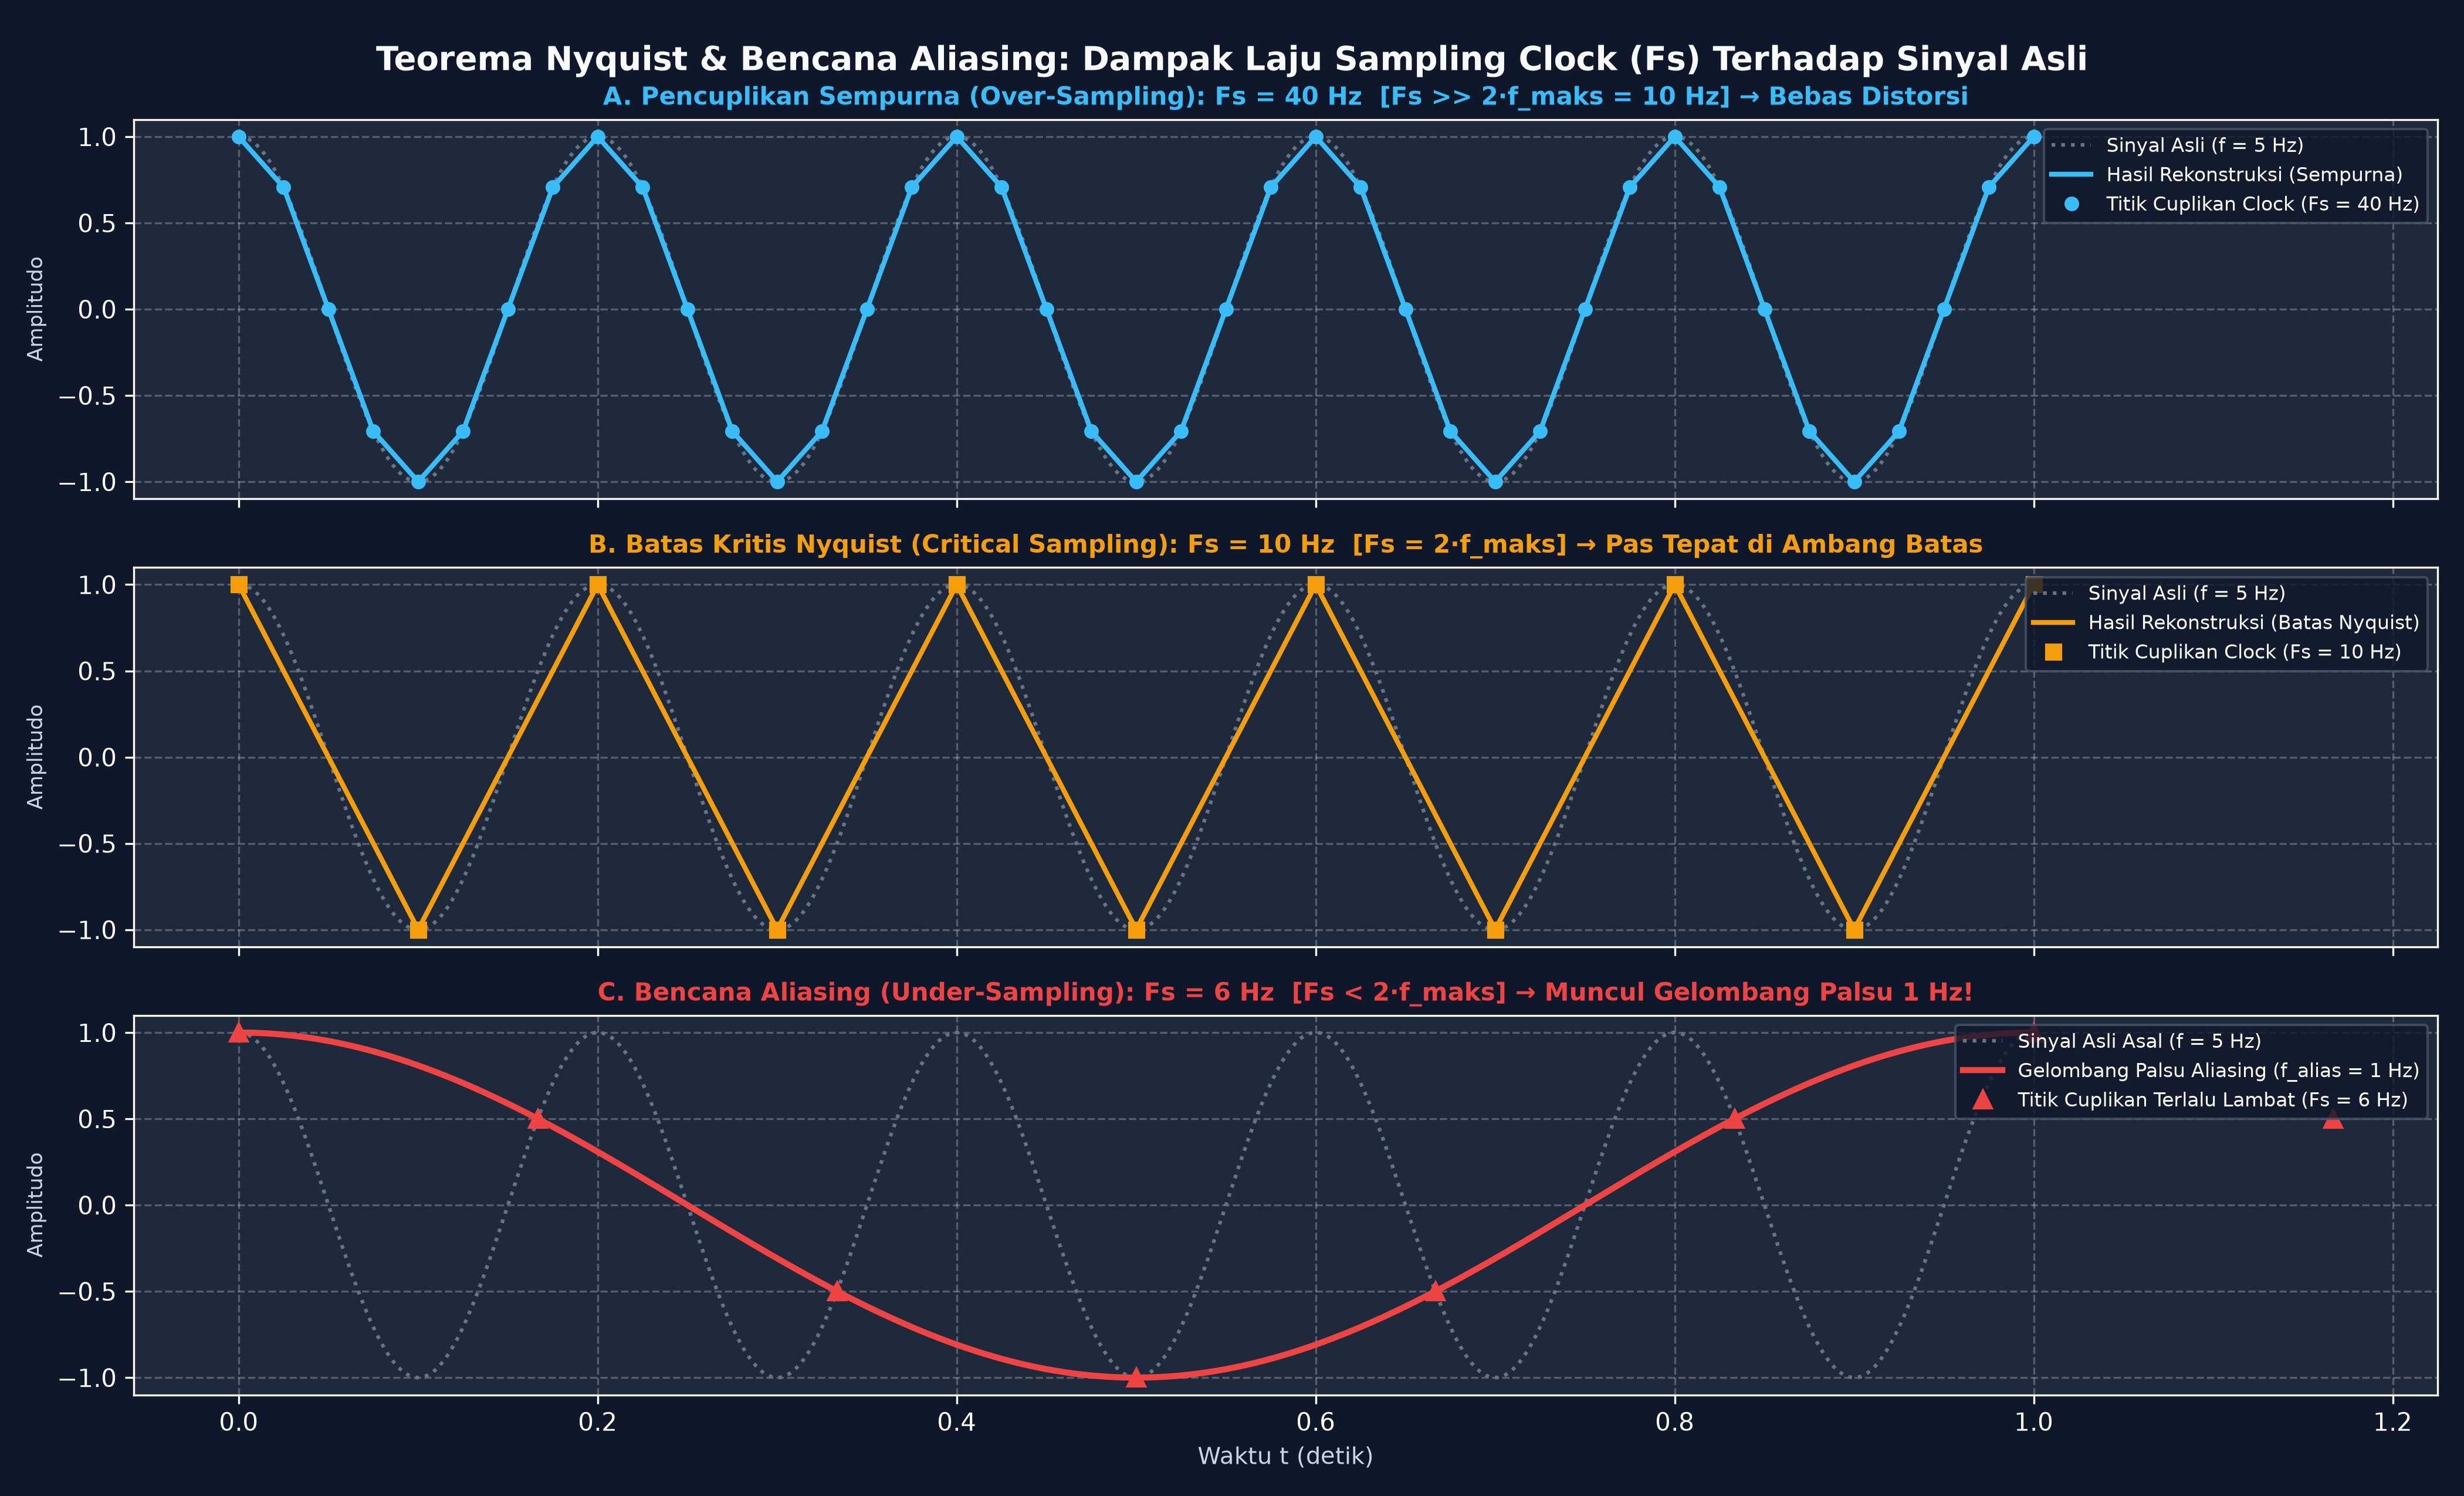
\includegraphics[width=0.95\linewidth]{assets/sampling_nyquist_aliasing.png}
  \captionof{figure}{Fenomena rekonstruksi gelombang terhadap variasi laju pencuplikan $F_s$ pada sinyal uji $f = 5\text{ Hz}$.}
\end{center}

\begin{analisisbox}[Derivasi Perilaku Tiga Kondisi Sampling]
\begin{itemize}[leftmargin=*]
  \item \textbf{Kondisi A — Over-Sampling ($F_s = 40\text{ Hz} \gg 2 f_{\max} = 10\text{ Hz}$):}  
  Replika spektral $X_a(F - k F_s)$ terpisah sejauh interval $40\text{ Hz}$ dengan pita transisi pelindung (*guard band*) selebar $\Delta F = F_s - 2 f_{\max} = 30\text{ Hz}$. Rekonstruksi gelombang melalui filter rekonstruksi ideal menghasilkan sinyal asli sempurna 100\% tanpa distorsi.

  \item \textbf{Kondisi B — Batas Kritis Nyquist ($F_s = 10\text{ Hz} = 2 f_{\max}$):}  
  Ujung-ujung spektrum replika tepat bersinggungan pada frekuensi lipat $f_{\text{fold}} = F_s / 2 = 5\text{ Hz}$. Rekonstruksi masih dimungkinkan secara teoritis menggunakan filter *brick-wall* ideal tanpa guard band.

  \item \textbf{Kondisi C — Bencana Under-Sampling \& Aliasing ($F_s = 6\text{ Hz} < 2 f_{\max}$):}  
  Spektrum replika mengalami tumpang tindih (*spectral overlapping*). Komponen frekuensi asli $F = +5\text{ Hz}$ terlipat masuk ke pita dasar $|F| \le F_s/2 = 3\text{ Hz}$ menghasilkan frekuensi semu alias:
  \begin{equation}
  f_{\text{alias}} = |F - 1 \cdot F_s| = |5\text{ Hz} - 6\text{ Hz}| = 1\text{ Hz}
  \end{equation}
  Komputer merekonstruksi gelombang hantu palsu berwarna merah pada frekuensi $1\text{ Hz}$ yang sama sekali tidak ada di dunia nyata!
\end{itemize}
\end{analisisbox}

\begin{teoremabox}[Teorema Sampling Nyquist-Shannon \& Interpolasi Whittaker-Shannon]
Jika sinyal kontinu $x_a(t)$ berpita terbatas pada rentang $-f_{\max} \le F \le f_{\max}$, maka $x_a(t)$ dapat dipulihkan secara eksak tanpa cacat dari sampel diskritnya $x[n] = x_a(n T_s)$ jika dan hanya jika $F_s \geq 2 f_{\max}$, dengan rumus rekonstruksi interpolasi sinus kardinal (Sinc):
\begin{equation}
x_a(t) = \sum_{n=-\infty}^{\infty} x[n] \operatorname{sinc}\left( \frac{t - n T_s}{T_s} \right) = \sum_{n=-\infty}^{\infty} x[n] \frac{\sin\left(\pi (t - n T_s)/T_s\right)}{\pi (t - n T_s)/T_s}
\end{equation}
\end{teoremabox}

\newpage
\subsection{Kuantisasi \& Pengkodean Biner 3-Bit (Rentang 0 s.d. 10 Volt)}

Kuantisasi seragam (*uniform quantization*) membagi rentang tegangan penuh $V_{\text{range}} = V_{\text{maks}} - V_{\text{min}}$ menjadi $L = 2^B$ sub-interval dengan lebar step $\Delta$:
\begin{equation}
\Delta = \frac{V_{\text{maks}} - V_{\text{min}}}{2^B} = \frac{10.0\text{ V} - 0.0\text{ V}}{2^3} = \frac{10.0\text{ V}}{8} = 1.25\text{ Volt / step}
\end{equation}

\begin{center}
  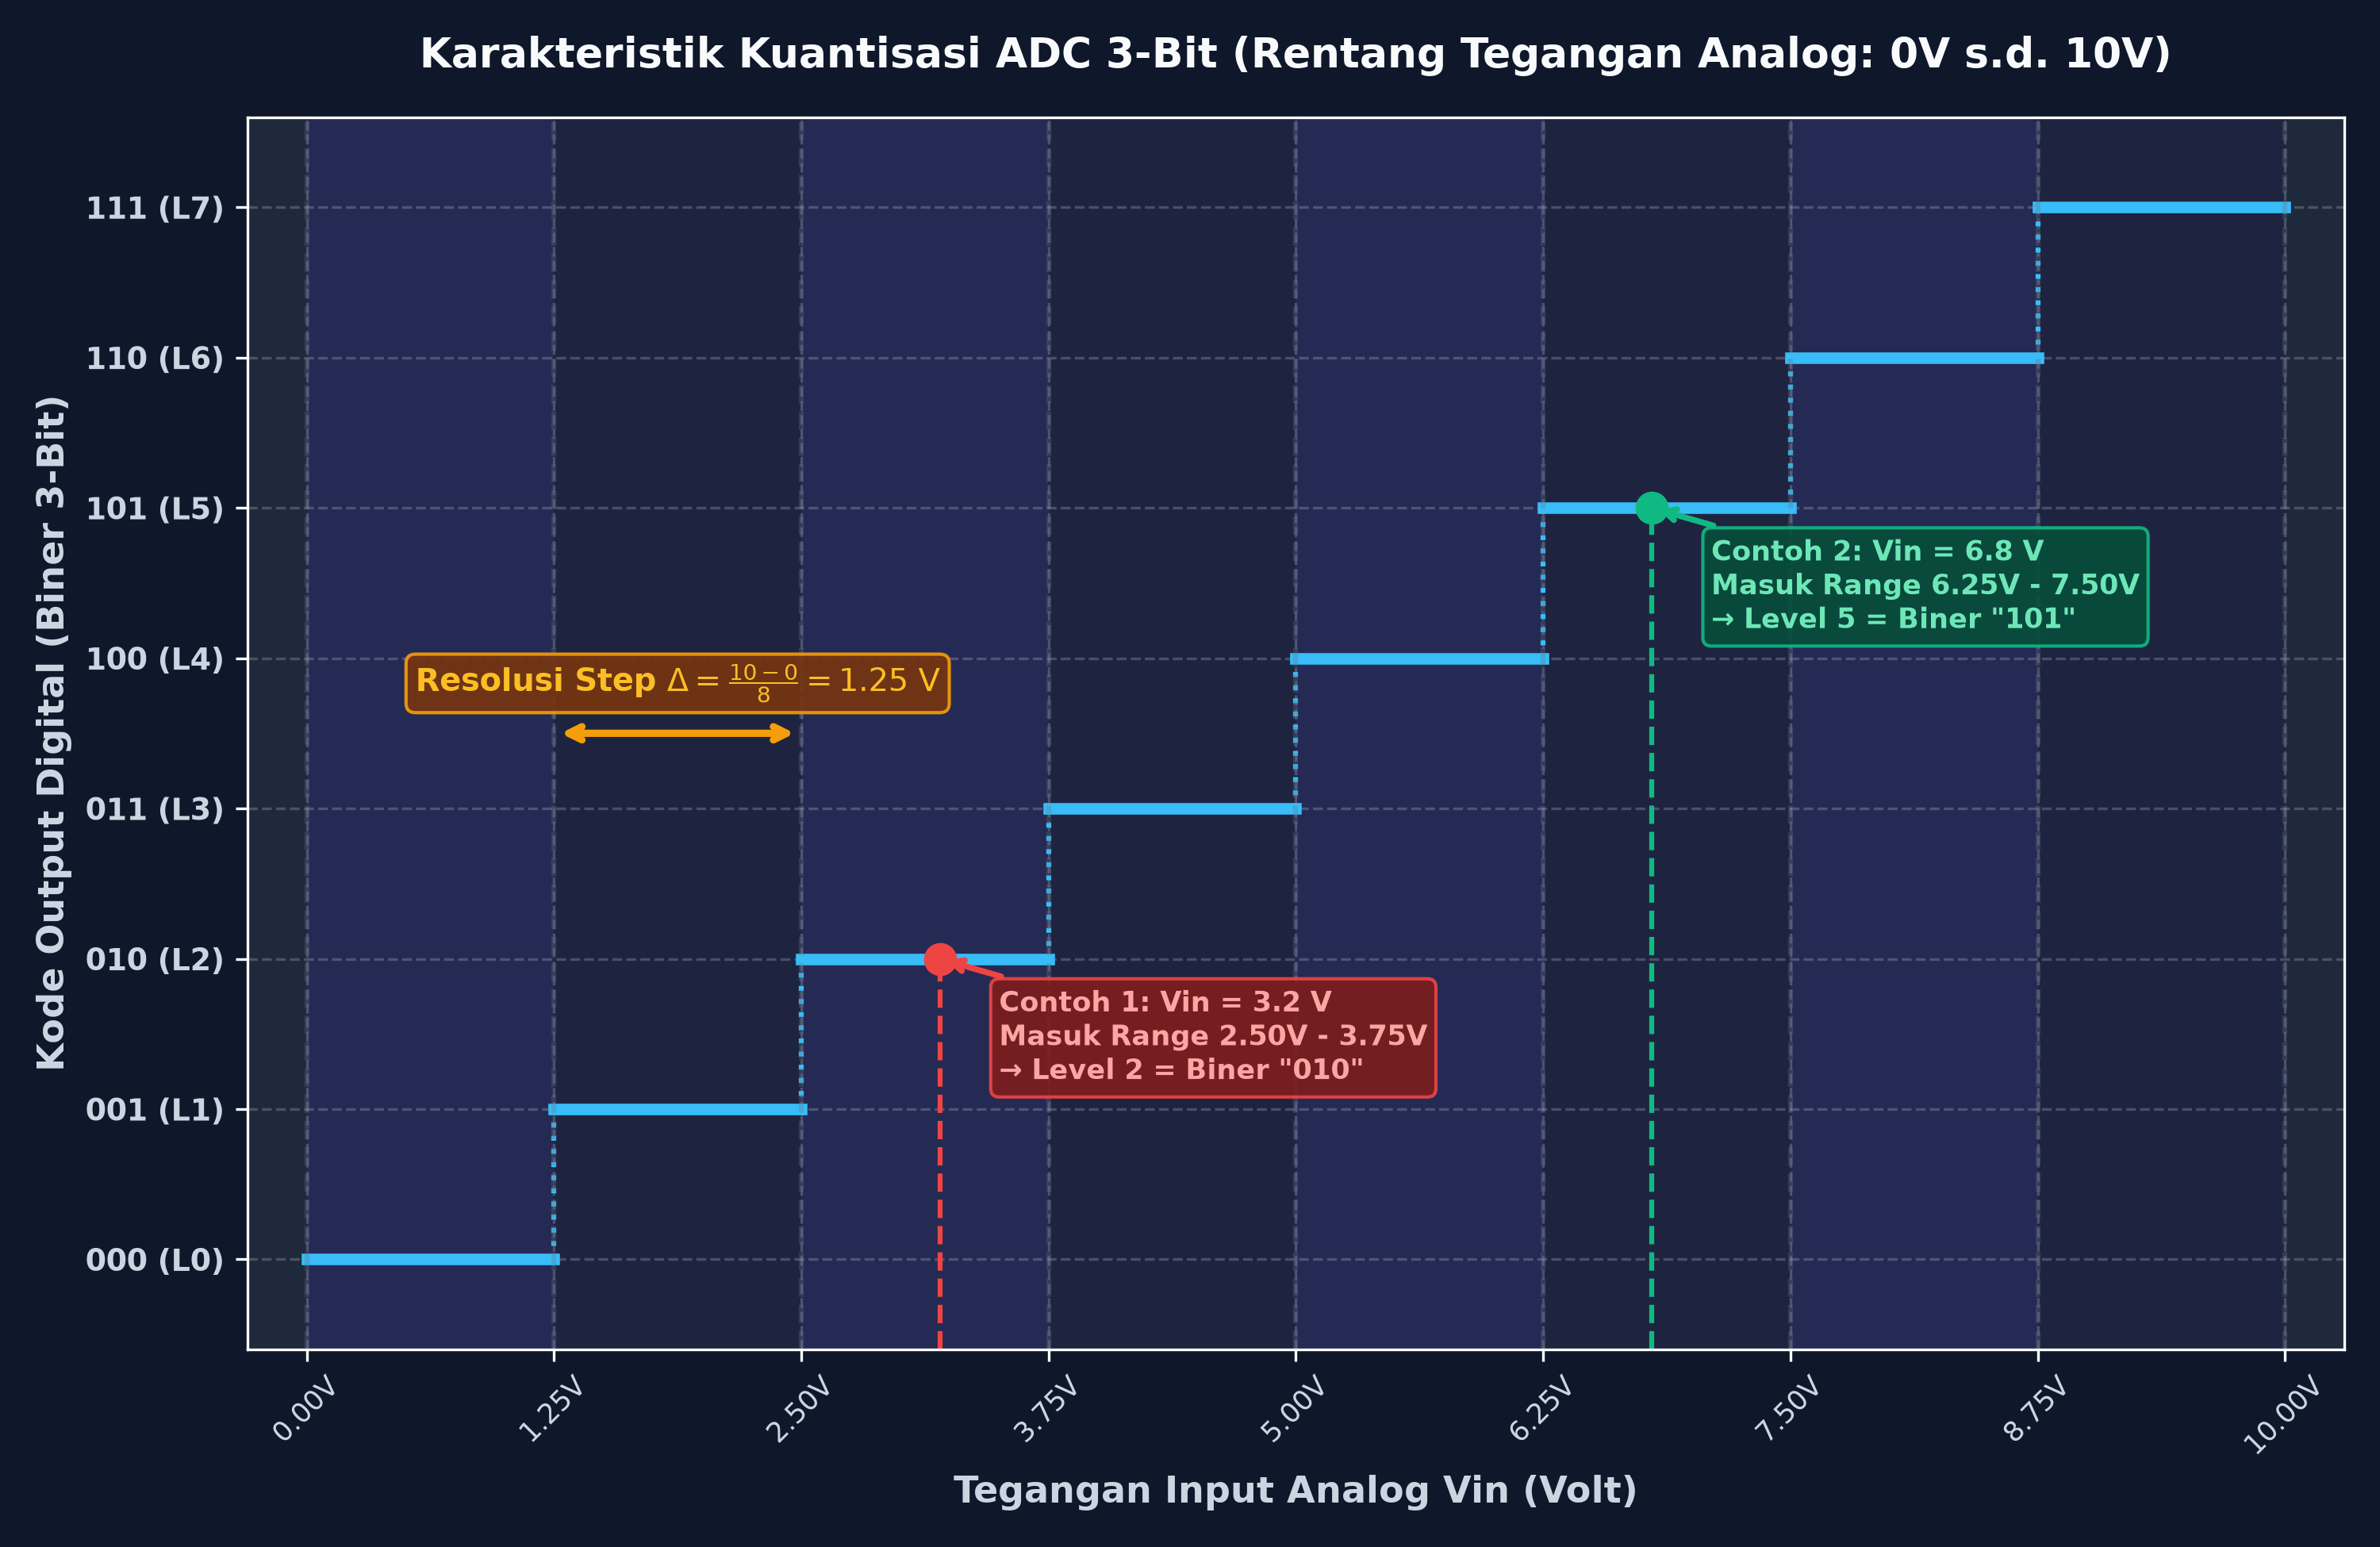
\includegraphics[width=0.90\linewidth]{assets/kuantisasi_3bit_0_10v.png}
  \captionof{figure}{Fungsi tangga kuantisasi uniform 3-bit: Titik batas partisi input, level representasi tengah $V_q$, dan error kuantisasi maksimal $\pm \Delta/2$.}
\end{center}

\begin{analisisbox}[Pemodelan Derau Kuantisasi \& Derivasi Formal Rasio SQNR]
Asumsikan galat kuantisasi $e_q[n] = x_q[n] - x[n]$ berdistribusi seragam kontinu pada interval $[-\Delta/2, +\Delta/2]$ dengan fungsi densitas probabilitas $f_E(e) = 1/\Delta$. Nilai rata-rata dan daya derau (variansi $\sigma_e^2$) dihitung sebagai:
\begin{equation}
\mu_e = \mathbb{E}[e] = 0, \qquad P_e = \sigma_e^2 = \mathbb{E}[e^2] = \int_{-\Delta/2}^{+\Delta/2} e^2 \cdot \frac{1}{\Delta} de = \left[ \frac{e^3}{3\Delta} \right]_{-\Delta/2}^{+\Delta/2} = \frac{\Delta^2}{12}
\end{equation}
Untuk sinyal input sinusoidal penuh yang mengisi seluruh rentang dinamis ADC $V_{\text{pp}} = 2^B \Delta$, amplitudonya $A = \frac{2^B \Delta}{2} = 2^{B-1}\Delta$. Daya rata-rata sinyal adalah:
\begin{equation}
P_s = \frac{A^2}{2} = \frac{(2^{B-1}\Delta)^2}{2} = \frac{2^{2B-2}\Delta^2}{2} = \frac{2^{2B}\Delta^2}{8}
\end{equation}
Rasio Daya Sinyal terhadap Derau Kuantisasi (*Signal-to-Quantization-Noise Ratio* / SQNR) dalam skala desibel (dB):
\begin{align}
\text{SQNR} &= 10 \log_{10}\left( \frac{P_s}{P_e} \right) = 10 \log_{10}\left( \frac{\frac{2^{2B}\Delta^2}{8}}{\frac{\Delta^2}{12}} \right) = 10 \log_{10}\left( \frac{12}{8} \cdot 2^{2B} \right) \nonumber \\
&= 10 \log_{10}(1.5) + 20 B \log_{10}(2) \approx \mathbf{6.02 \cdot B + 1.76 \quad [\text{dB}]}
\end{align}
\textit{Aturan Praktis (Rule of Thumb):} Setiap penambahan $1\text{ bit}$ resolusi ADC meningkatkan kualitas sinyal sebesar $\approx 6.02\text{ dB}$ (mereduksi daya derau kuantisasi hingga $1/4$ atau $\approx 75\%$).
\end{analisisbox}

\begin{table}[h!]
\centering
\small
\caption{Tabel Pemetaan Partisi \& Nilai Tengah Kuantisasi 3-Bit ($0 - 10\text{ V}, \Delta = 1.25\text{ V}$)}
\begin{tabularx}{\textwidth}{>{\centering\arraybackslash}m{2.0cm} >{\centering\arraybackslash}X >{\centering\arraybackslash}m{2.0cm} >{\centering\arraybackslash}m{3.2cm} >{\centering\arraybackslash}m{2.5cm}}
\toprule
\textbf{Step Kuantisasi} & \textbf{Rentang Partisi Masukan ($V_{\text{in}}$)} & \textbf{Kode Biner} & \textbf{Level Representasi ($V_q$)} & \textbf{Error Maks ($\pm \Delta/2$)} \\
\midrule
\textbf{Step 1} & $0.00\text{ V} \leq V_{\text{in}} < 1.25\text{ V}$ & \texttt{000} & $0.625\text{ V}$ & $\pm 0.625\text{ V}$ \\
\textbf{Step 2} & $1.25\text{ V} \leq V_{\text{in}} < 2.50\text{ V}$ & \texttt{001} & $1.875\text{ V}$ & $\pm 0.625\text{ V}$ \\
\textbf{Step 3} & $2.50\text{ V} \leq V_{\text{in}} < 3.75\text{ V}$ & \texttt{010} & $3.125\text{ V}$ & $\pm 0.625\text{ V}$ \\
\textbf{Step 4} & $3.75\text{ V} \leq V_{\text{in}} < 5.00\text{ V}$ & \texttt{011} & $4.375\text{ V}$ & $\pm 0.625\text{ V}$ \\
\textbf{Step 5} & $5.00\text{ V} \leq V_{\text{in}} < 6.25\text{ V}$ & \texttt{100} & $5.625\text{ V}$ & $\pm 0.625\text{ V}$ \\
\textbf{Step 6} & $6.25\text{ V} \leq V_{\text{in}} < 7.50\text{ V}$ & \texttt{101} & $6.875\text{ V}$ & $\pm 0.625\text{ V}$ \\
\textbf{Step 7} & $7.50\text{ V} \leq V_{\text{in}} < 8.75\text{ V}$ & \texttt{110} & $8.125\text{ V}$ & $\pm 0.625\text{ V}$ \\
\textbf{Step 8} & $8.75\text{ V} \leq V_{\text{in}} \leq 10.00\text{ V}$ & \texttt{111} & $9.375\text{ V}$ & $\pm 0.625\text{ V}$ \\
\bottomrule
\end{tabularx}
\end{table}

\newpage
\subsection{Studi Kasus End-to-End: Konversi Sinyal Sinus ke Aliran Bit Biner}

Diberikan sinyal input analog: $x(t) = 5.0 + 4.0 \sin(2\pi \cdot 1.0 \cdot t)\text{ Volt}$, disampling dengan laju $F_s = 8\text{ Hz}$ ($T_s = 0.125\text{ s}$) pada sistem ADC 3-bit ($0 - 10\text{ V}, \Delta = 1.25\text{ V}$).

\begin{center}
  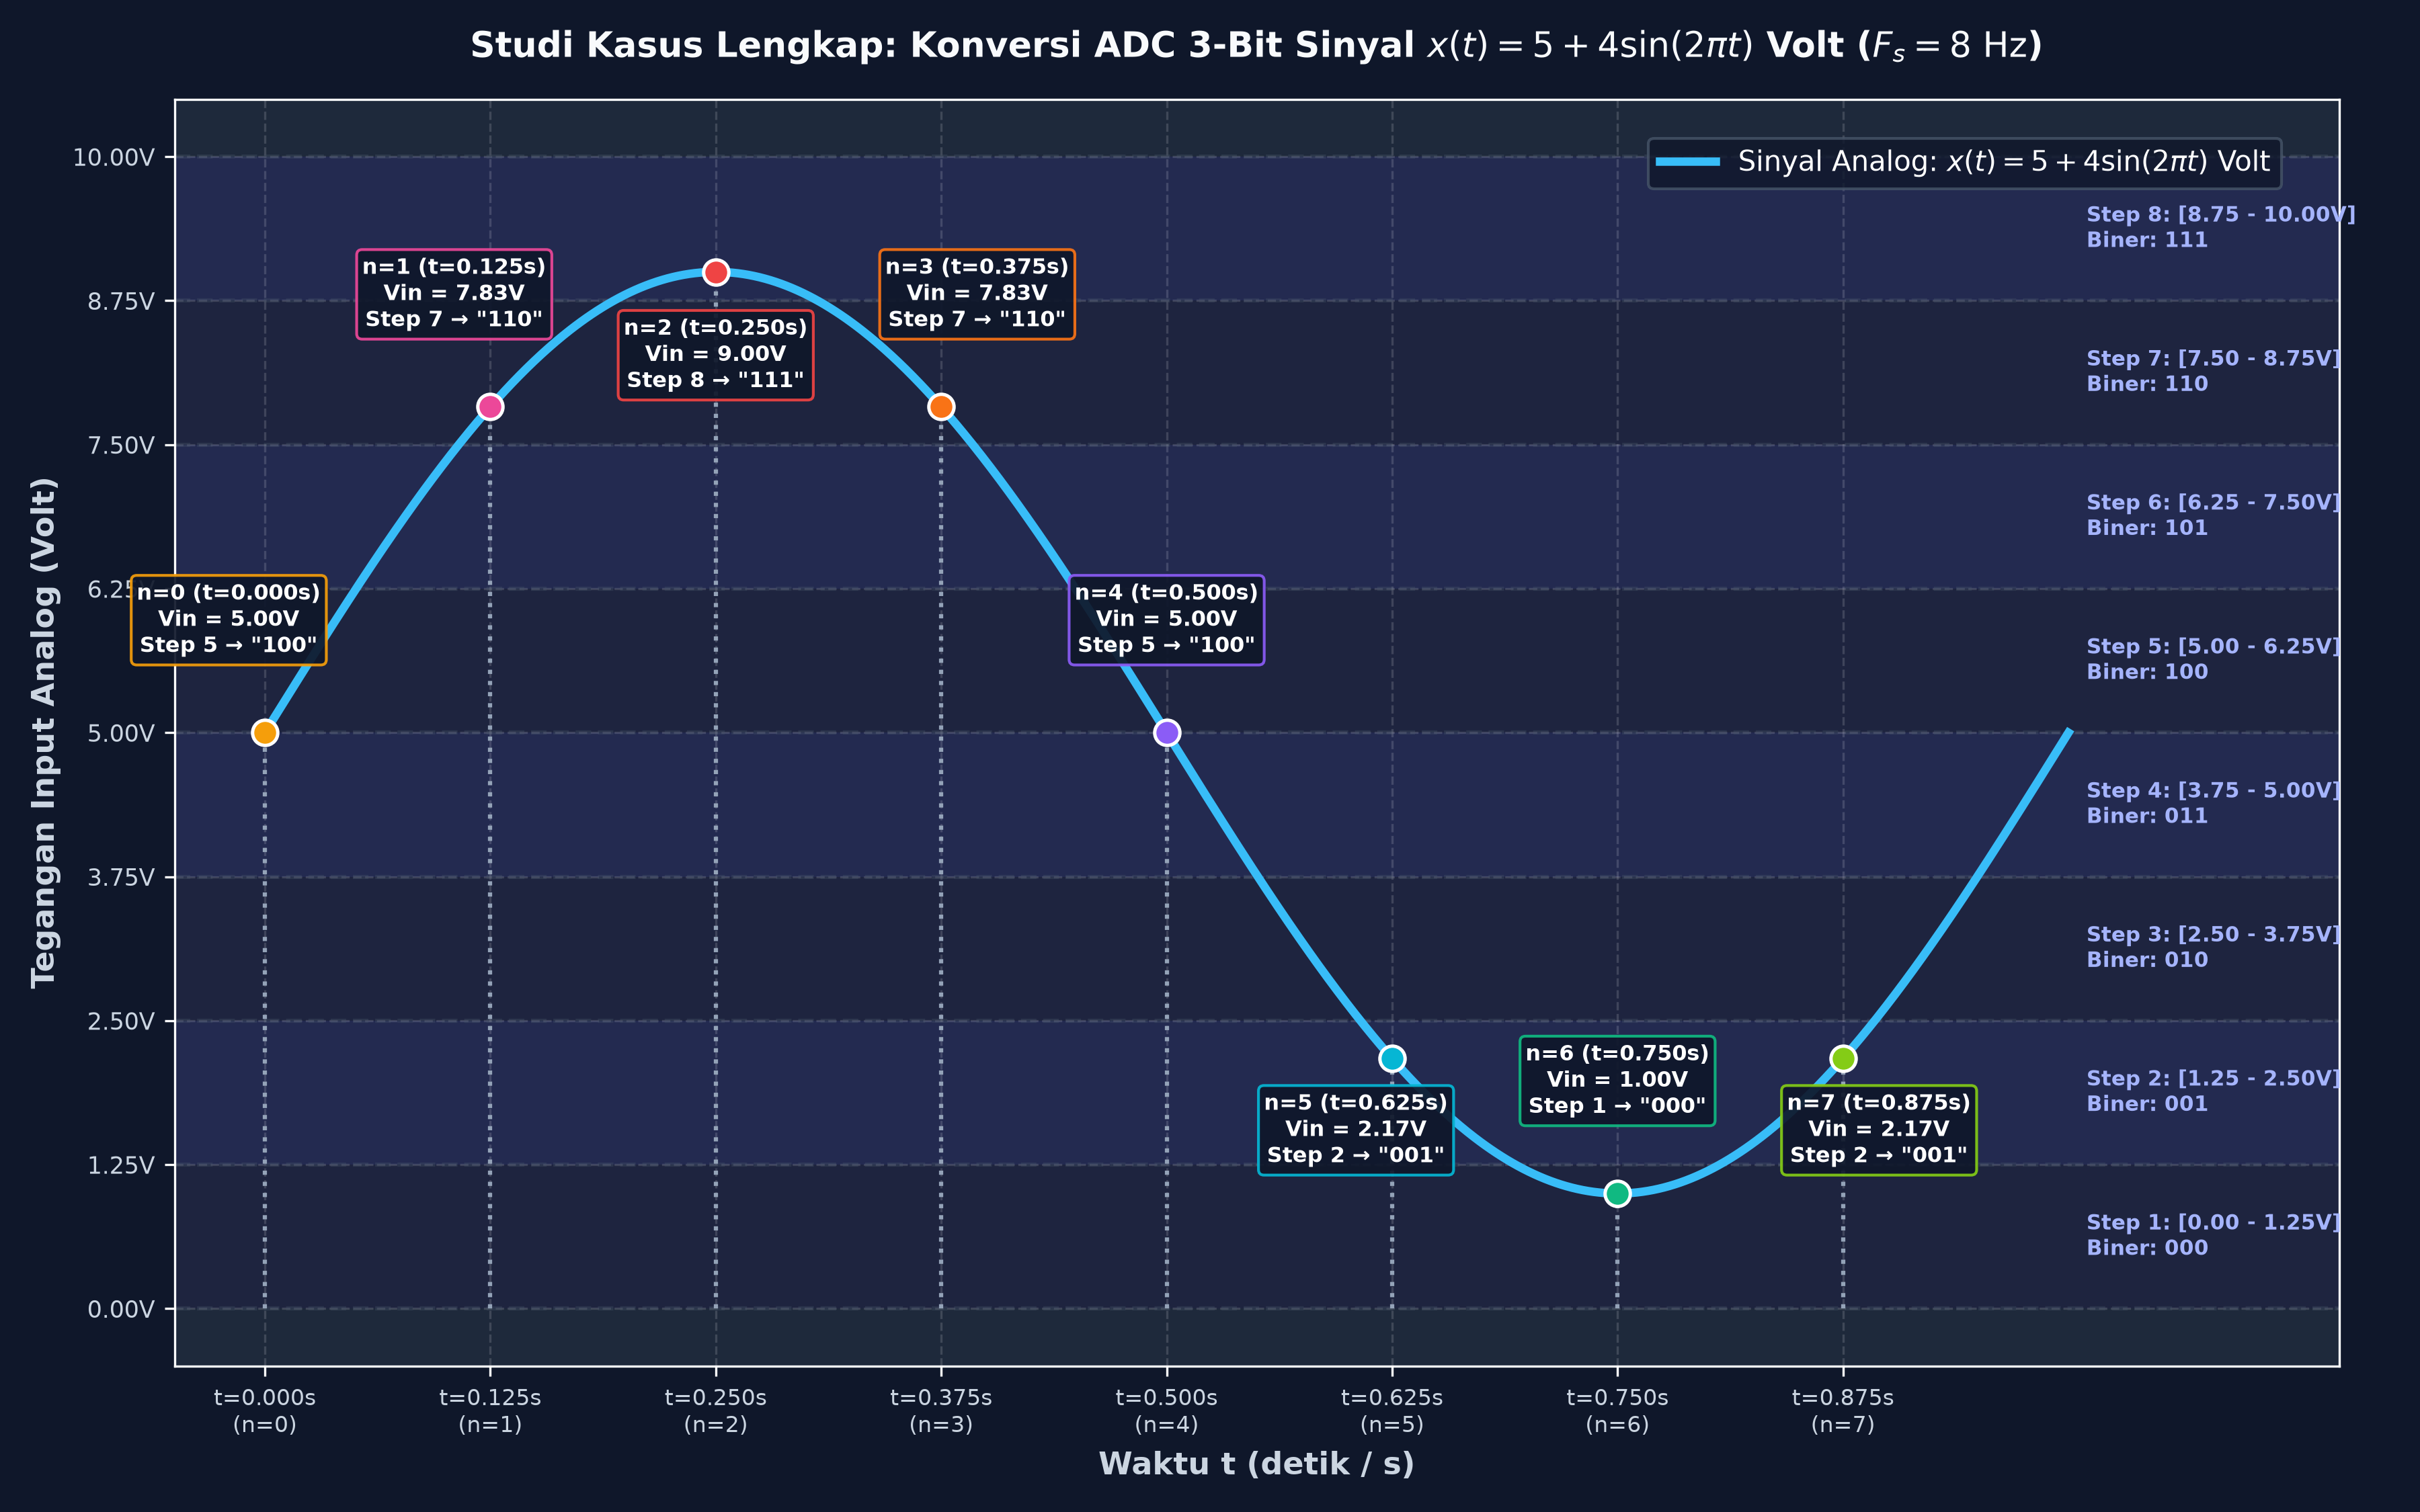
\includegraphics[width=0.95\linewidth]{assets/studi_kasus_konversi_lengkap.png}
  \captionof{figure}{Pelacakan titik-ke-titik dari sinyal analog kontinu menuju sampel diskrit waktu, kuantisasi, galat $e_q[n]$, dan bitstream biner serial.}
\end{center}

\begin{analisisbox}[Tabel Kalkulasi Numerik Eksak 8 Titik Sampel ($n=0 \dots 7$)]
\begin{center}
\small
\begin{tabularx}{\textwidth}{>{\centering\arraybackslash}m{1.4cm} >{\centering\arraybackslash}m{1.6cm} >{\centering\arraybackslash}X >{\centering\arraybackslash}m{2.3cm} >{\centering\arraybackslash}m{2.1cm} >{\centering\arraybackslash}m{1.5cm}}
\toprule
\textbf{Indeks $n$} & \textbf{Waktu $t_n$} & \textbf{Tegangan Eksak $x(t_n)$} & \textbf{Step \& Level $V_q$} & \textbf{Galat $e_q[n]$} & \textbf{Biner} \\
\midrule
$n = 0$ & $0.000\text{ s}$ & $5.000\text{ V}$ & Step 5 ($5.625\text{ V}$) & $+0.625\text{ V}$ & \texttt{100} \\
$n = 1$ & $0.125\text{ s}$ & $5 + 4\sin(\pi/4) = 7.828\text{ V}$ & Step 7 ($8.125\text{ V}$) & $+0.297\text{ V}$ & \texttt{110} \\
$n = 2$ & $0.250\text{ s}$ & $5 + 4\sin(\pi/2) = 9.000\text{ V}$ & Step 8 ($9.375\text{ V}$) & $+0.375\text{ V}$ & \texttt{111} \\
$n = 3$ & $0.375\text{ s}$ & $5 + 4\sin(3\pi/4) = 7.828\text{ V}$ & Step 7 ($8.125\text{ V}$) & $+0.297\text{ V}$ & \texttt{110} \\
$n = 4$ & $0.500\text{ s}$ & $5 + 4\sin(\pi) = 5.000\text{ V}$ & Step 5 ($5.625\text{ V}$) & $+0.625\text{ V}$ & \texttt{100} \\
$n = 5$ & $0.625\text{ s}$ & $5 + 4\sin(5\pi/4) = 2.172\text{ V}$ & Step 2 ($1.875\text{ V}$) & $-0.297\text{ V}$ & \texttt{001} \\
$n = 6$ & $0.750\text{ s}$ & $5 + 4\sin(3\pi/2) = 1.000\text{ V}$ & Step 1 ($0.625\text{ V}$) & $-0.375\text{ V}$ & \texttt{000} \\
$n = 7$ & $0.875\text{ s}$ & $5 + 4\sin(7\pi/4) = 2.172\text{ V}$ & Step 2 ($1.875\text{ V}$) & $-0.297\text{ V}$ & \texttt{001} \\
\bottomrule
\end{tabularx}
\end{center}

\vspace{0.2cm}
\textbf{Evaluasi Rata-rata Galat Kuadrat (Mean Squared Error / MSE):}
\begin{align}
\text{MSE} &= \frac{1}{8}\sum_{n=0}^7 (e_q[n])^2 = \frac{2(0.625)^2 + 4(0.297)^2 + 2(0.375)^2}{8} \nonumber \\
&= \frac{0.78125 + 0.35284 + 0.28125}{8} \approx \mathbf{0.1769\ \text{V}^2}
\end{align}
\textbf{Aliran Bit Biner Serial Output (Bitstream):}
\[
\mathbf{\text{Bitstream Serial}} = \mathbf{\underbrace{100}_{n=0} \ \underbrace{110}_{n=1} \ \underbrace{111}_{n=2} \ \underbrace{110}_{n=3} \ \underbrace{100}_{n=4} \ \underbrace{001}_{n=5} \ \underbrace{000}_{n=6} \ \underbrace{001}_{n=7}} \quad (24\text{ bit per siklus})
\]
\end{analisisbox}

\newpage
% =========================================================================
\section{Klasifikasi Lanjutan Sinyal Modern}
% =========================================================================

\subsection{Sinyal Multikanal (Multi-Channel Signals) \& Representasi Vektor-Matriks}

Dalam sistem akuisisi sinyal canggih seperti EEG 64-kanal, susunan mikrofon *Beamforming*, dan radar MIMO (*Multiple-Input Multiple-Output*), data direkam secara simultan oleh array $M$ sensor spasial.

\begin{center}
  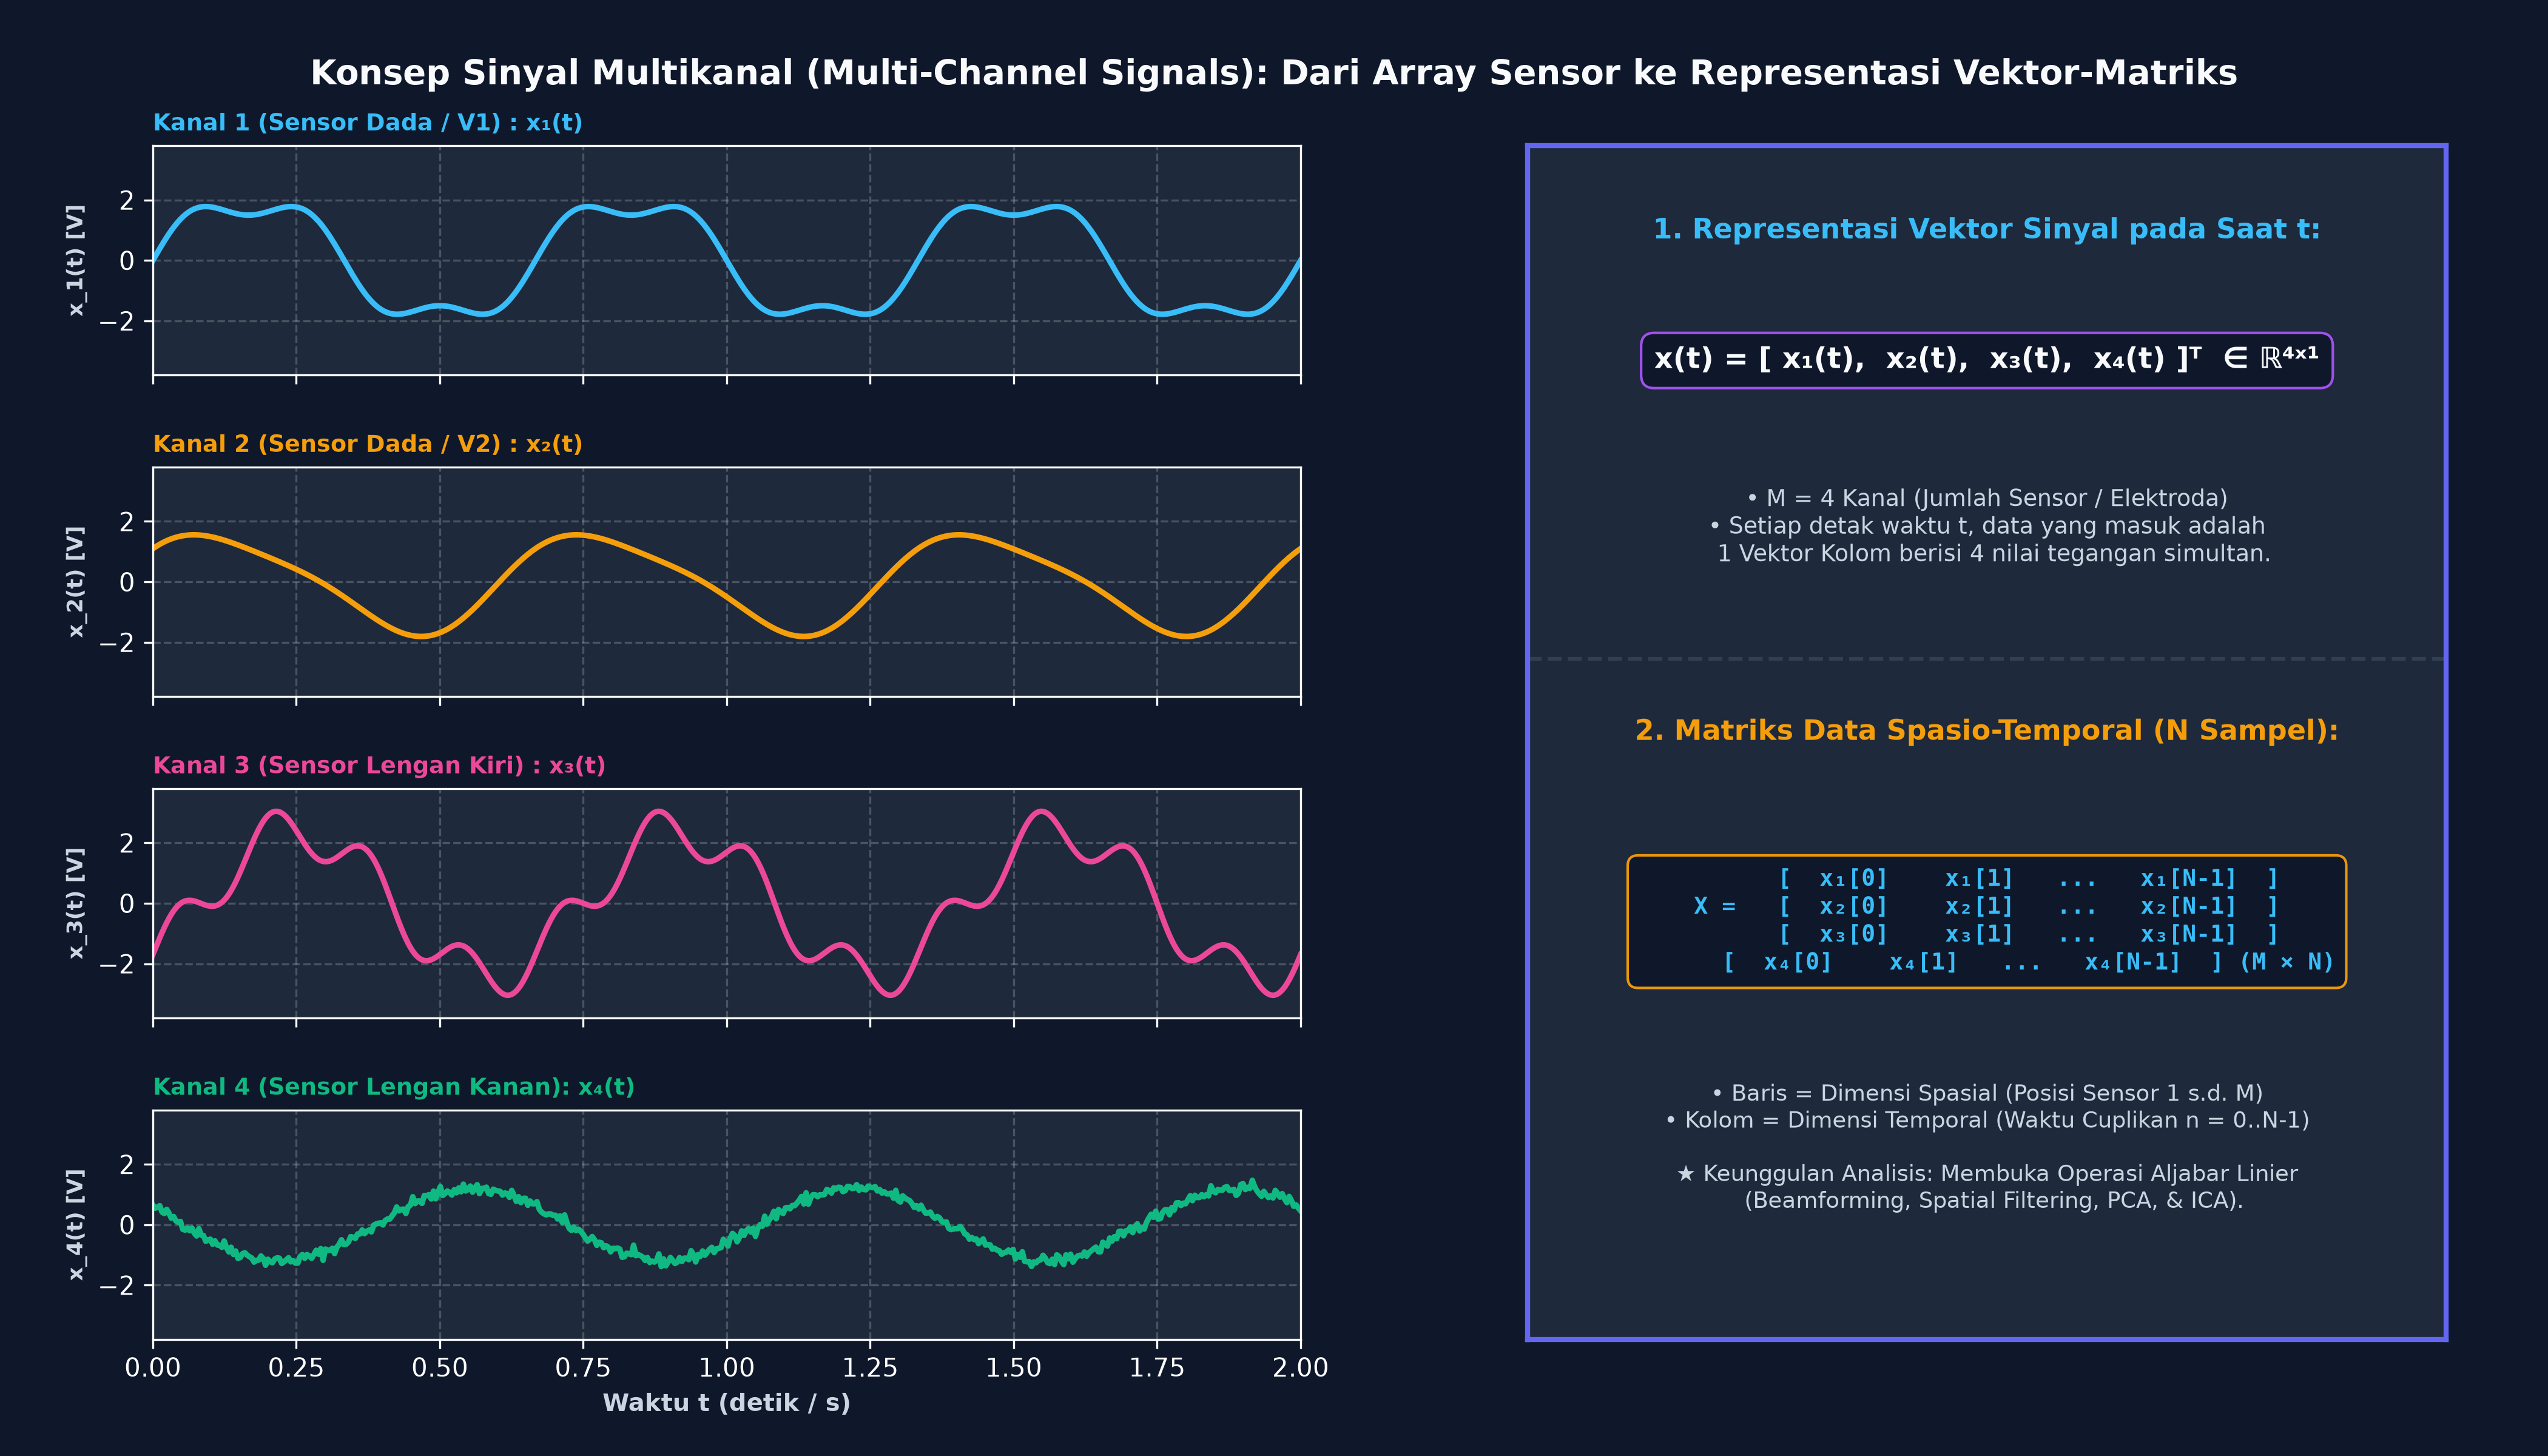
\includegraphics[width=0.92\linewidth]{assets/sinyal_multikanal.png}
  \captionof{figure}{Akuisisi Sinyal Multikanal 4-kanal EKG simultan dan pemetaannya ke struktur aljabar matriks spasio-temporal $\mathbf{X}_{M \times N}$.}
\end{center}

\begin{analisisbox}[Formulasi Aljabar Linear Sinyal Multikanal]
\begin{itemize}[leftmargin=*]
  \item \textbf{Vektor Kolom Cuplikan Spasial pada Detak Waktu $n$:}
  \begin{equation}
  \mathbf{x}[n] = \begin{bmatrix} x_1[n] \\ x_2[n] \\ \vdots \\ x_M[n] \end{bmatrix} \in \mathbb{R}^{M \times 1}, \quad \text{untuk } n = 0, 1, \dots, N-1
  \end{equation}
  \item \textbf{Matriks Spasio-Temporal $\mathbf{X}_{M \times N}$:}
  \begin{equation}
  \mathbf{X} = \begin{bmatrix} \mathbf{x}[0] & \mathbf{x}[1] & \cdots & \mathbf{x}[N-1] \end{bmatrix} = \begin{bmatrix} 
  x_1[0] & x_1[1] & \cdots & x_1[N-1] \\
  x_2[0] & x_2[1] & \cdots & x_2[N-1] \\
  \vdots & \vdots & \ddots & \vdots \\
  x_M[0] & x_M[1] & \cdots & x_M[N-1]
  \end{bmatrix} \in \mathbb{R}^{M \times N}
  \end{equation}
  \item \textbf{Matriks Korelasi Spasial ($\mathbf{R}_{xx}$) \& Pemisahan Sumber Sinyal:}  
  Struktur kovariansi antar-sensor dihitung melalui:
  \begin{equation}
  \mathbf{R}_{xx} = \frac{1}{N} \mathbf{X} \mathbf{X}^T \in \mathbb{R}^{M \times M}
  \end{equation}
  Melalui Dekomposisi Nilai Singular (SVD) $\mathbf{X} = \mathbf{U} \mathbf{\Sigma} \mathbf{V}^T$, vektor basis ortogonal $\mathbf{U}$ memisahkan sumber interferensi artefak gerak dari sinyal biomedis murni (*Principal Component Analysis* / PCA).
\end{itemize}
\end{analisisbox}

\vspace{0.3cm}
\subsection{Sinyal Multi-Dimensi (Multi-Dimensional Signals / M-D): 1D, 2D, 3D, hingga 4D}

Dimensi suatu sinyal didefinisikan secara matematis oleh derajat kebebasan atau banyaknya variabel bebas independen yang dipetakan oleh fungsi sinyal.

\begin{center}
  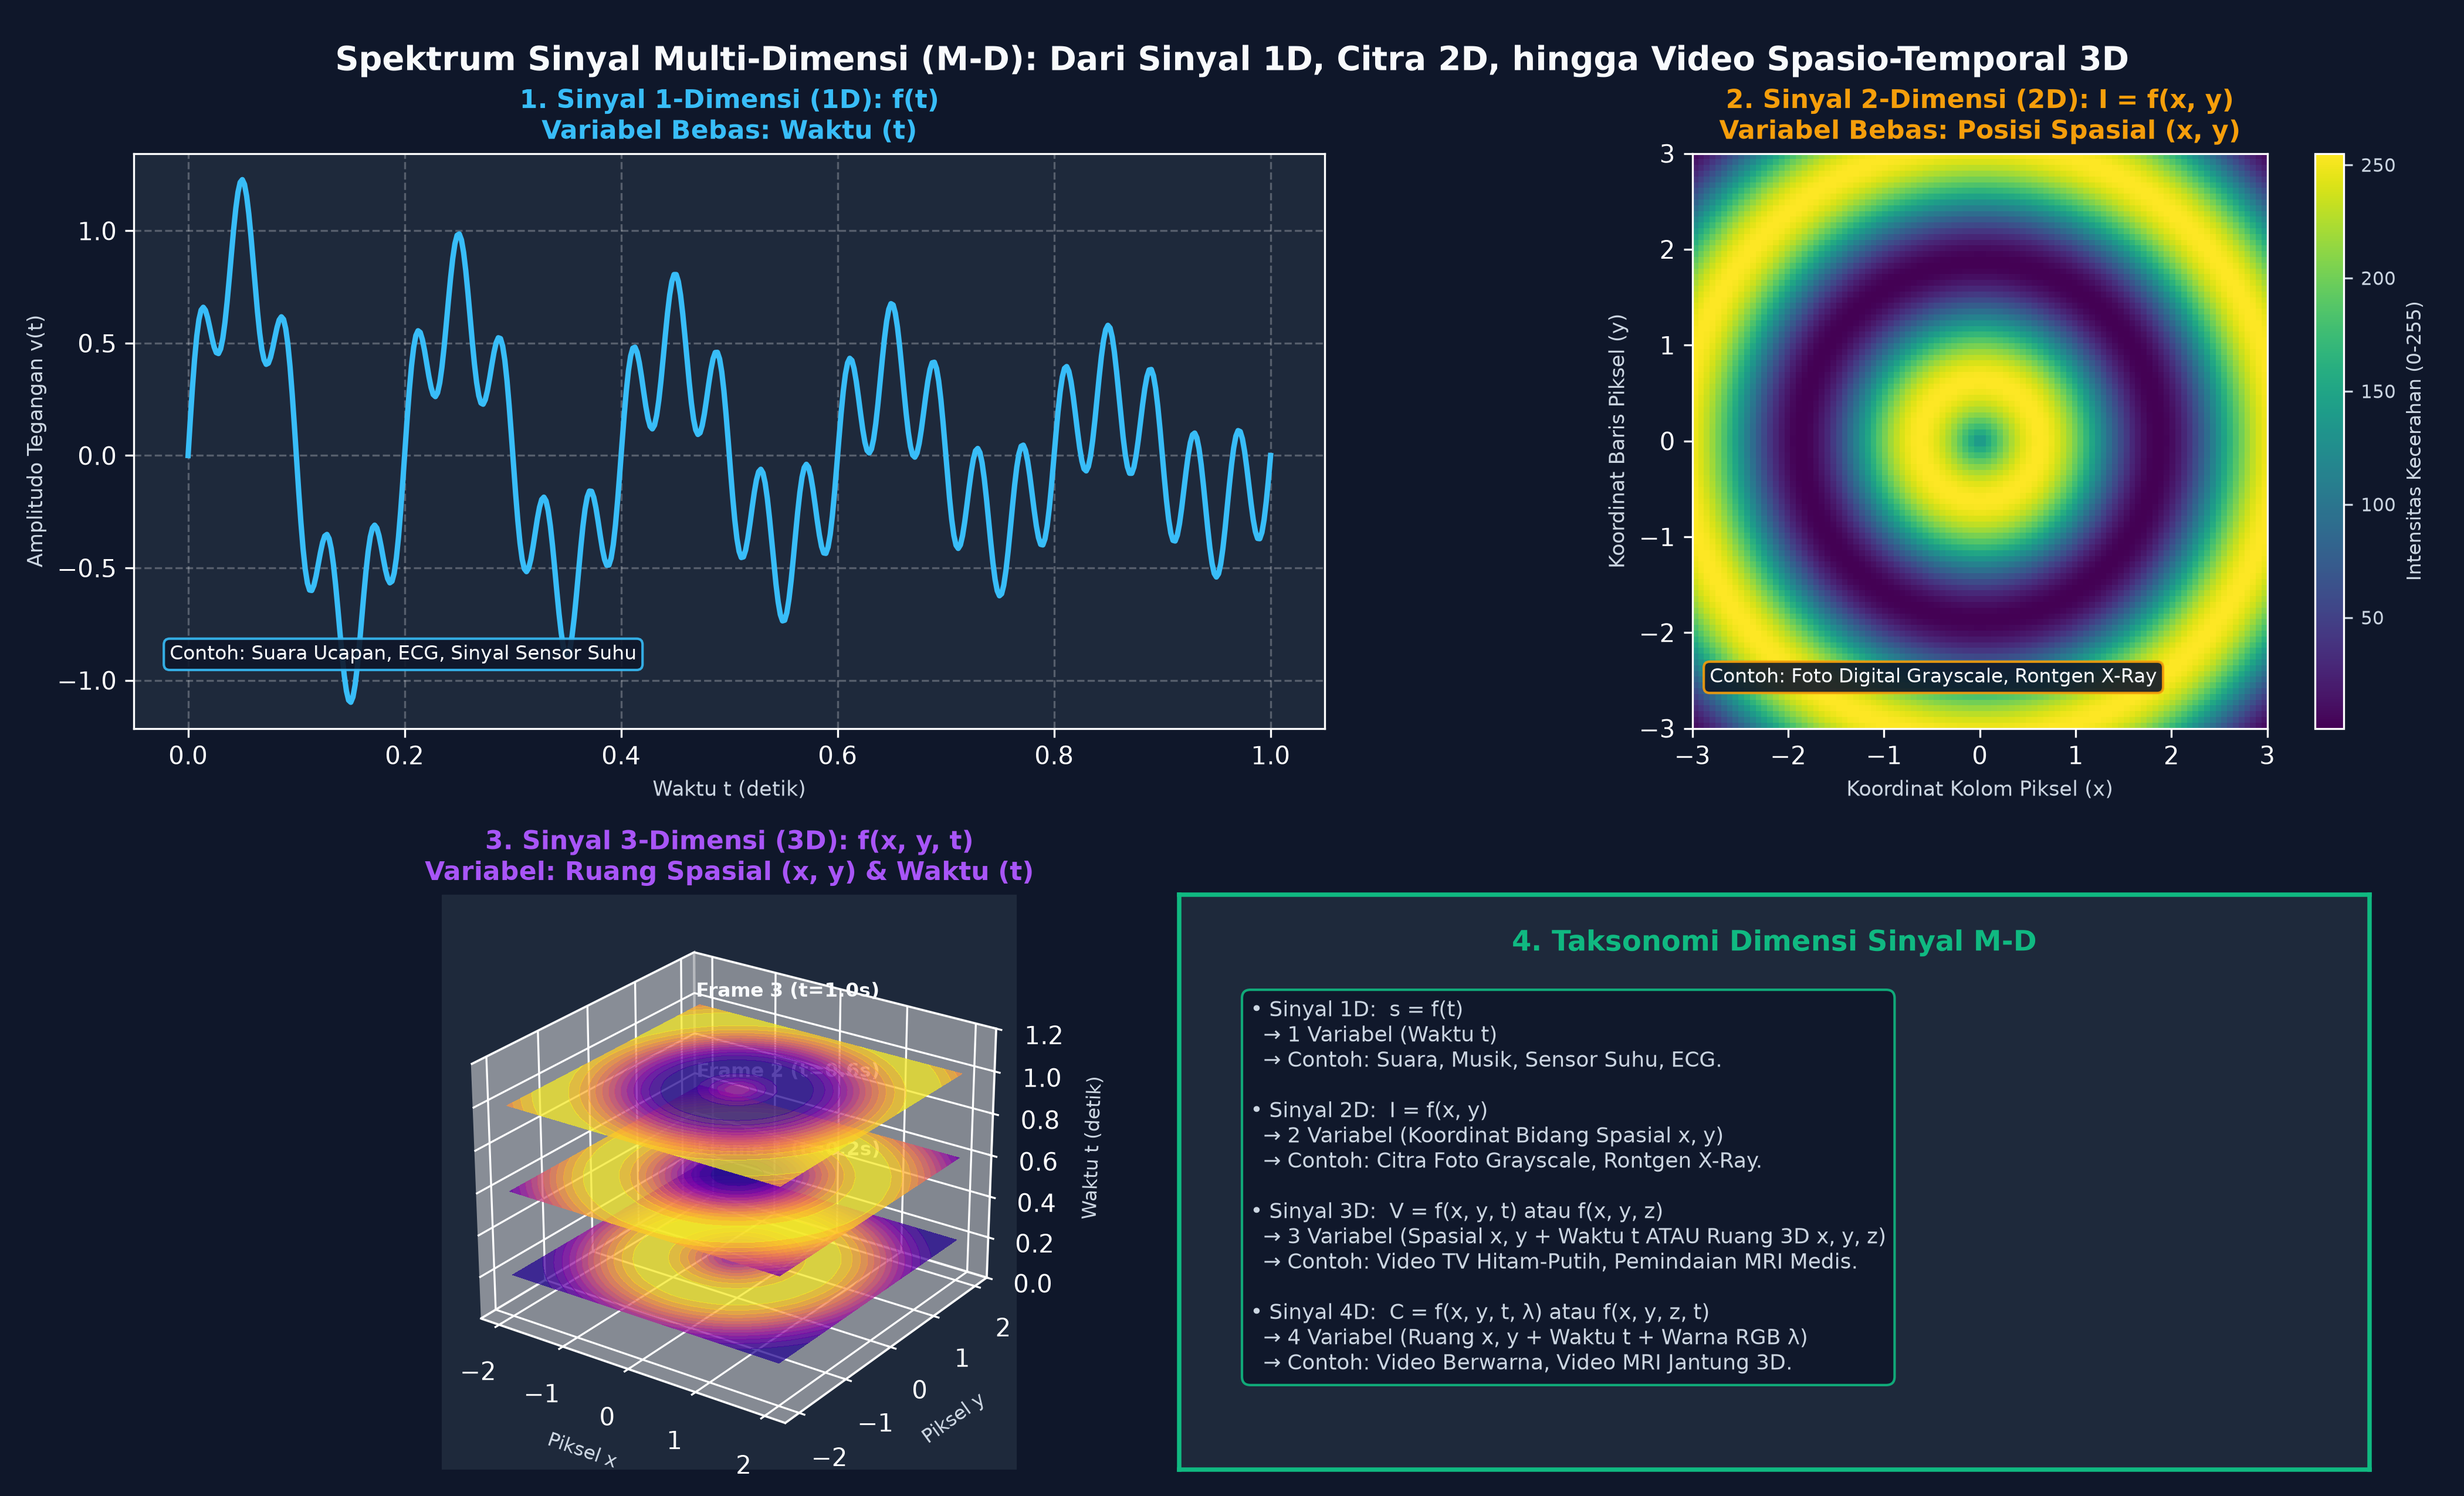
\includegraphics[width=0.95\linewidth]{assets/sinyal_multidimensi.png}
  \captionof{figure}{Hierarki sinyal Multi-Dimensi (M-D): 1D Audio $f(t)$, 2D Citra $f(x,y)$, 3D Spasio-Temporal $f(x,y,t)$, dan 4D Spektral $f(x,y,t,\lambda)$.}
\end{center}

\begin{analisisbox}[Klasifikasi Matematis \& Ruang Domain Sinyal M-D]
\begin{enumerate}[leftmargin=*]
  \item \textbf{Sinyal 1-Dimensi ($s: \mathbb{R} \to \mathbb{R}$):} Fungsi bergantung pada variabel tunggal (waktu $t$). Contoh: rekaman ucapan fonetik $s = f(t)$.
  \item \textbf{Sinyal 2-Dimensi ($I: \mathbb{R}^2 \to \mathbb{R}$):} Fungsi intensitas luminansi terdefinisi pada koordinat kartesius bidang spasial $(x,y)$. Transformasi Fourier 2-D sinyal kontinu dinyatakan:
  \begin{equation}
  F(u, v) = \int_{-\infty}^{\infty} \int_{-\infty}^{\infty} I(x, y) e^{-j 2\pi (ux + vy)} dx dy
  \end{equation}
  \item \textbf{Sinyal 3-Dimensi ($V: \mathbb{R}^3 \to \mathbb{R}$):} Memiliki 3 variabel bebas, seperti koordinat spasial-temporal video monokrom $V = f(x, y, t)$ atau volume tomografi 3-D medan magnetik MRI $V = f(x, y, z)$.
  \item \textbf{Sinyal 4-Dimensi ($C: \mathbb{R}^4 \to \mathbb{R}$):} Menggabungkan ruang $(x,y)$, waktu $(t)$, dan dimensi spektral panjang gelombang fotometrik $(\lambda)$ pada citra satelit hyperspectral atau video RGB berwarna bioskop $C(x, y, t, \lambda_c)$ di mana $\lambda_c \in \{\text{Red}, \text{Green}, \text{Blue}\}$.
\end{enumerate}
\end{analisisbox}

\newpage
\subsection{Sinyal Waktu Diskrit (Discrete-Time Signals / DTS) \& Sinyal Elementer}

Sinyal waktu diskrit $x[n]$ adalah barisan bilangan (*sequence*) yang terdefinisi hanya pada indeks integer bulat $n \in \mathbb{Z}$.

\begin{center}
  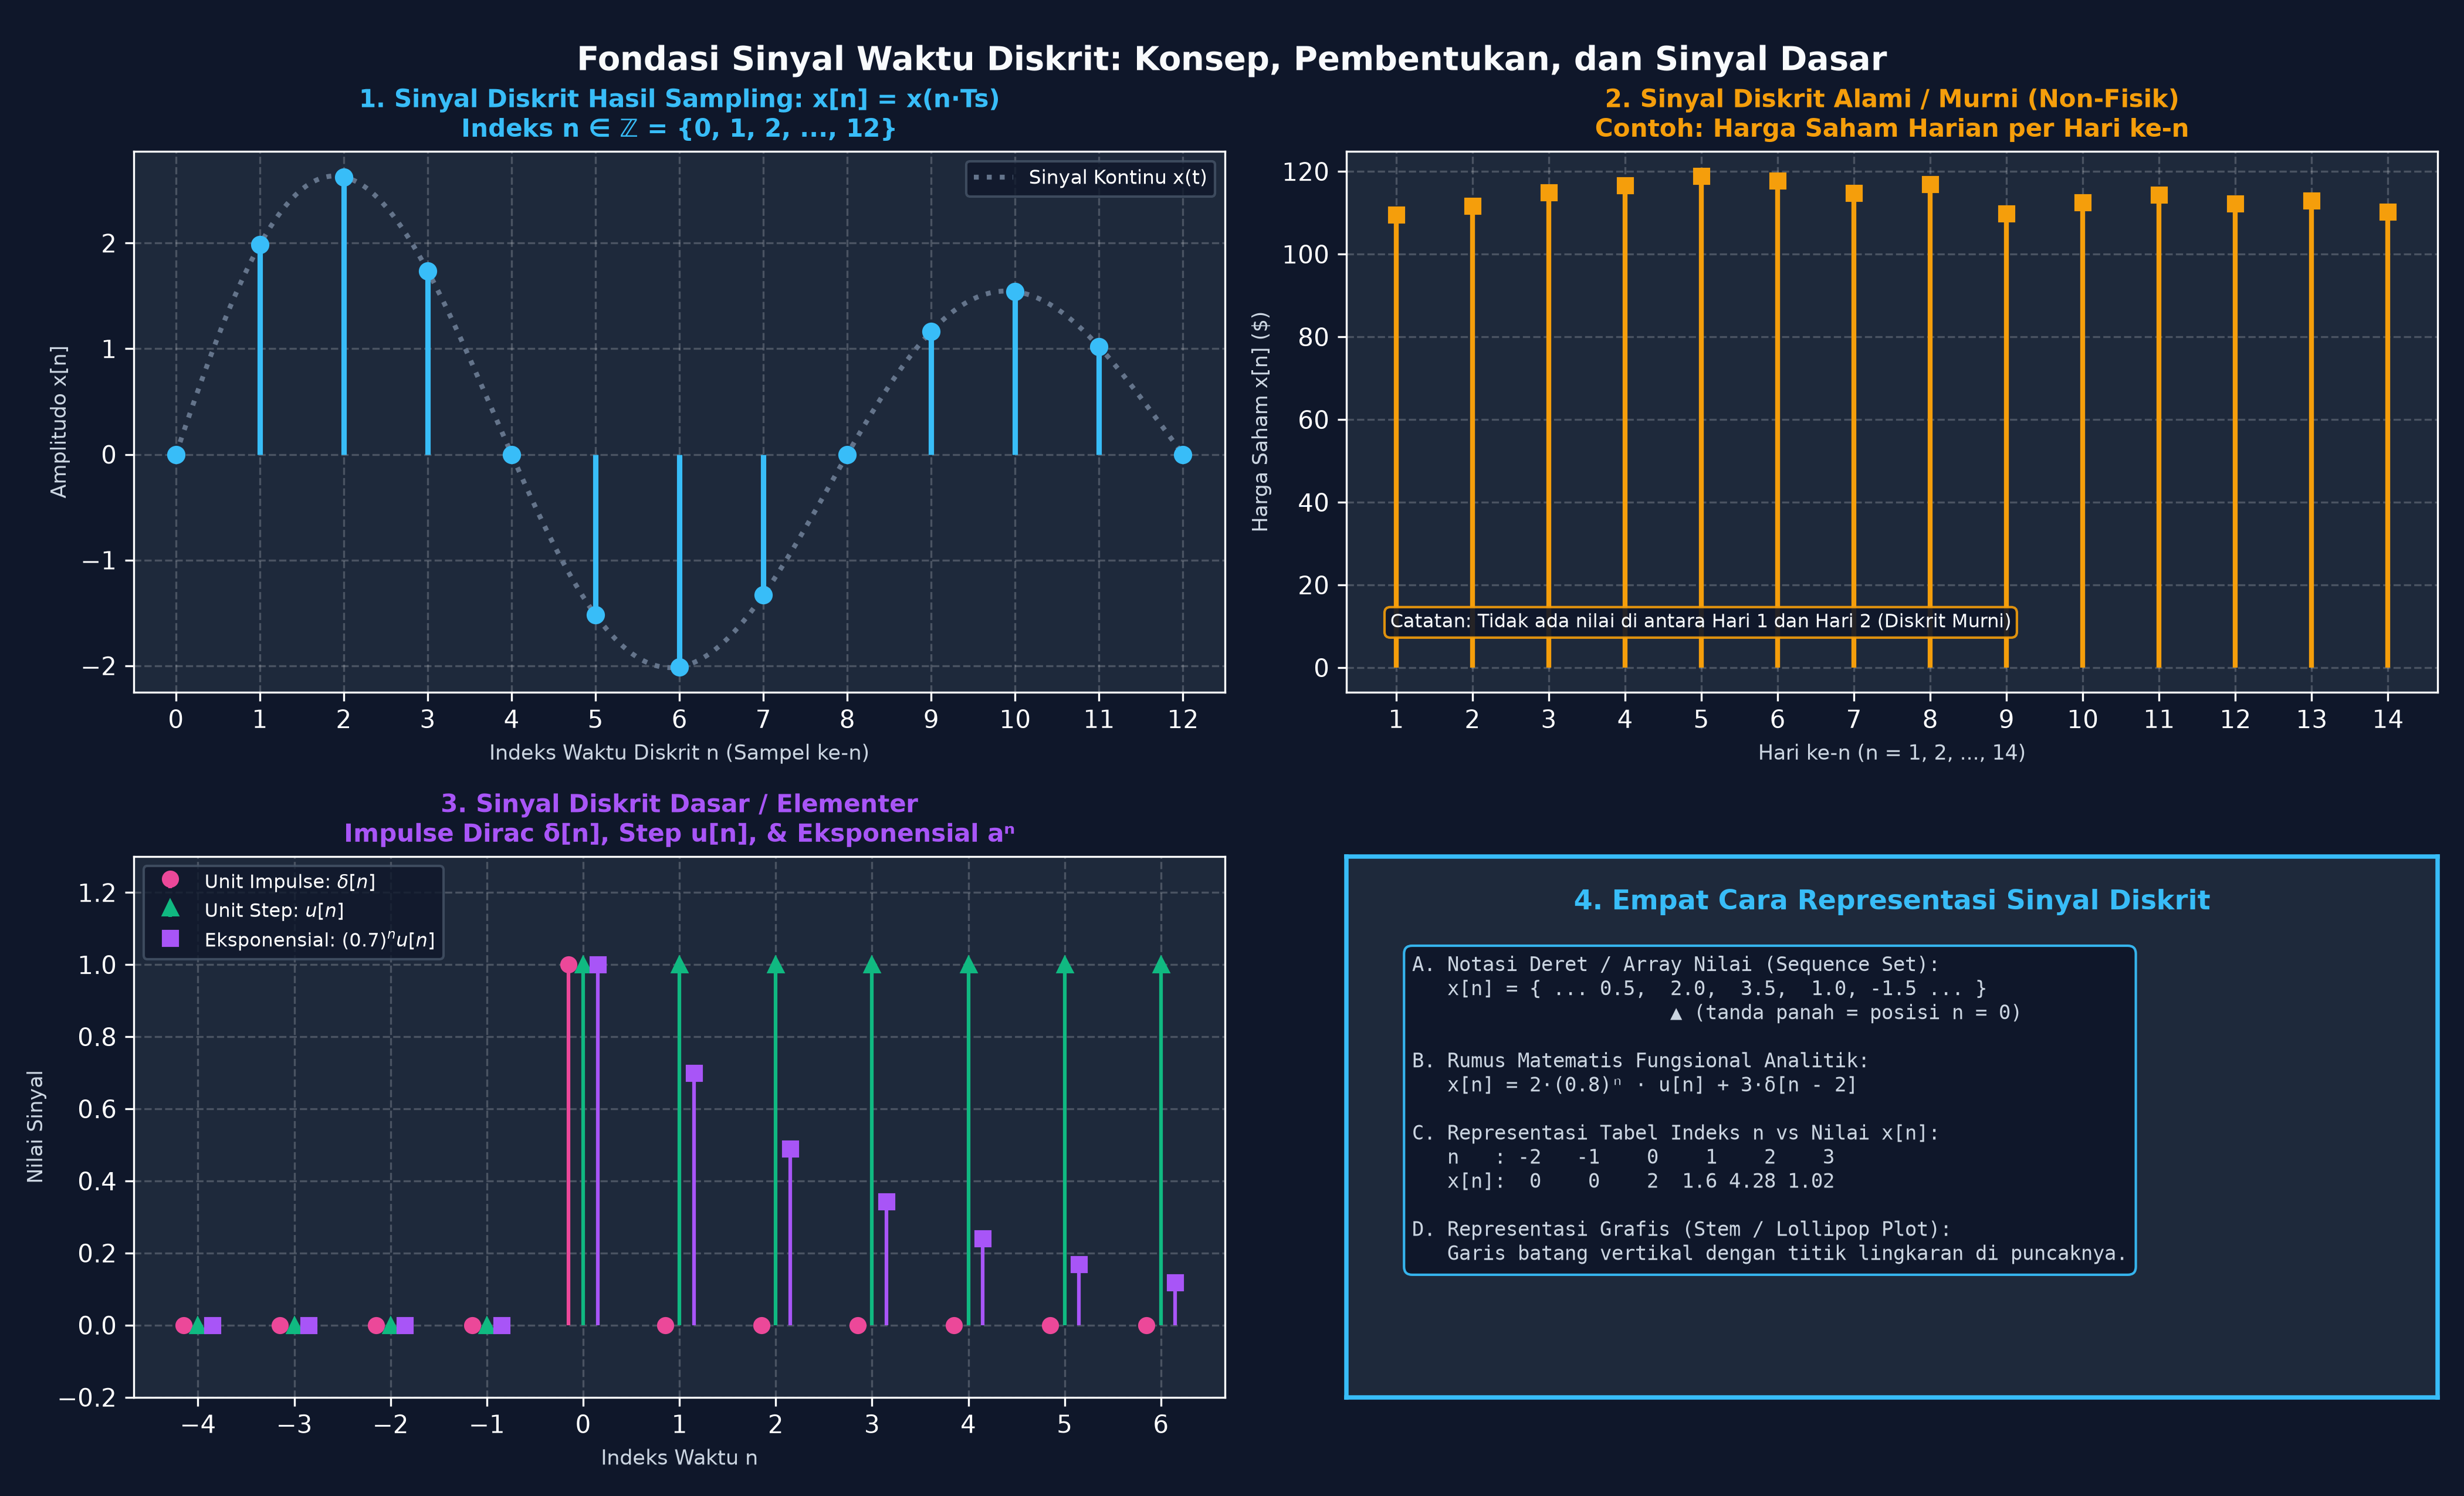
\includegraphics[width=0.95\linewidth]{assets/sinyal_waktu_diskrit.png}
  \captionof{figure}{Representasi Sinyal Waktu Diskrit (Stem Plot Sampling, Fluktuasi Diskrit Finansial) dan Tiga Sinyal Elementer Fundamental.}
\end{center}

\begin{analisisbox}[Dekomposisi Sinyal \& Sifat Tiga Sinyal Elementer]
\begin{enumerate}[leftmargin=*]
  \item \textbf{Sinyal Impuls Satuan / Kronecker Delta ($\delta[n]$):}
  \begin{equation}
  \delta[n] = \begin{cases} 1, & n = 0 \\ 0, & n \neq 0 \end{cases}
  \end{equation}
  \textit{Sifat Penyaringan (Sifting Property):} Sembarang sinyal diskrit $x[n]$ dapat didekomposisi menjadi kombinasi linier tak terhingga dari impuls-impuls tergeser dan terbobot:
  \begin{equation}
  \mathbf{x[n] = \sum_{k=-\infty}^{\infty} x[k] \delta[n - k]}
  \end{equation}
  
  \item \textbf{Sinyal Undak Satuan (Unit Step $u[n]$):}
  \begin{equation}
  u[n] = \begin{cases} 1, & n \ge 0 \\ 0, & n < 0 \end{cases} \equiv \sum_{k=-\infty}^n \delta[k]
  \end{equation}
  Hubungan diferensial diskrit (selisih maju): $\delta[n] = u[n] - u[n-1]$.

  \item \textbf{Sinyal Eksponensial Diskrit Riil \& Kompleks ($x[n] = a^n u[n]$):}  
  Untuk $a \in \mathbb{R}$: jika $|a| < 1$ kurva meluruh asimtotik (Panel 3 kurva ungu $0.7^n$); jika $a < 0$ tanda nilai berosilasi bolak-balik $\operatorname{sgn}(x[n]) = (-1)^n$. Jika $a = e^{\sigma_0 + j\omega_0} \in \mathbb{C}$, sinyal menghasilkan osilasi sinusoidal teredam/tumbuh $x[n] = e^{\sigma_0 n} \cos(\omega_0 n) u[n]$.
\end{enumerate}
\end{analisisbox}

% =========================================================================
\section{Klasifikasi Ruang Nilai \& Kepastian Sinyal}
% =========================================================================

\subsection{Definisi Hakiki Sinyal Digital: Diskrit Waktu \& Diskrit Amplitudo (4 Ruang Sinyal)}

\begin{definisibox}[Definisi Baku Sinyal Digital dalam Ruang Metrik Diskrit]
\textbf{Sinyal Digital} adalah sinyal yang berada dalam himpunan pemetaan metrik diskrit ganda:
\begin{equation}
x_d: \mathbb{Z} \to \mathbb{D}_L, \quad \text{di mana } \mathbb{D}_L = \{V_1, V_2, \dots, V_L\} \subset \mathbb{R}, \quad L = 2^B < \infty
\end{equation}
yang berarti sinyal telah mengalami diskritisasi variabel waktu independen ($n \in \mathbb{Z}$) dan sekaligus diskritisasi himpunan nilai dependen ($x_q[n]$) ke dalam kuantisasi berhingga.
\end{definisibox}

\begin{center}
  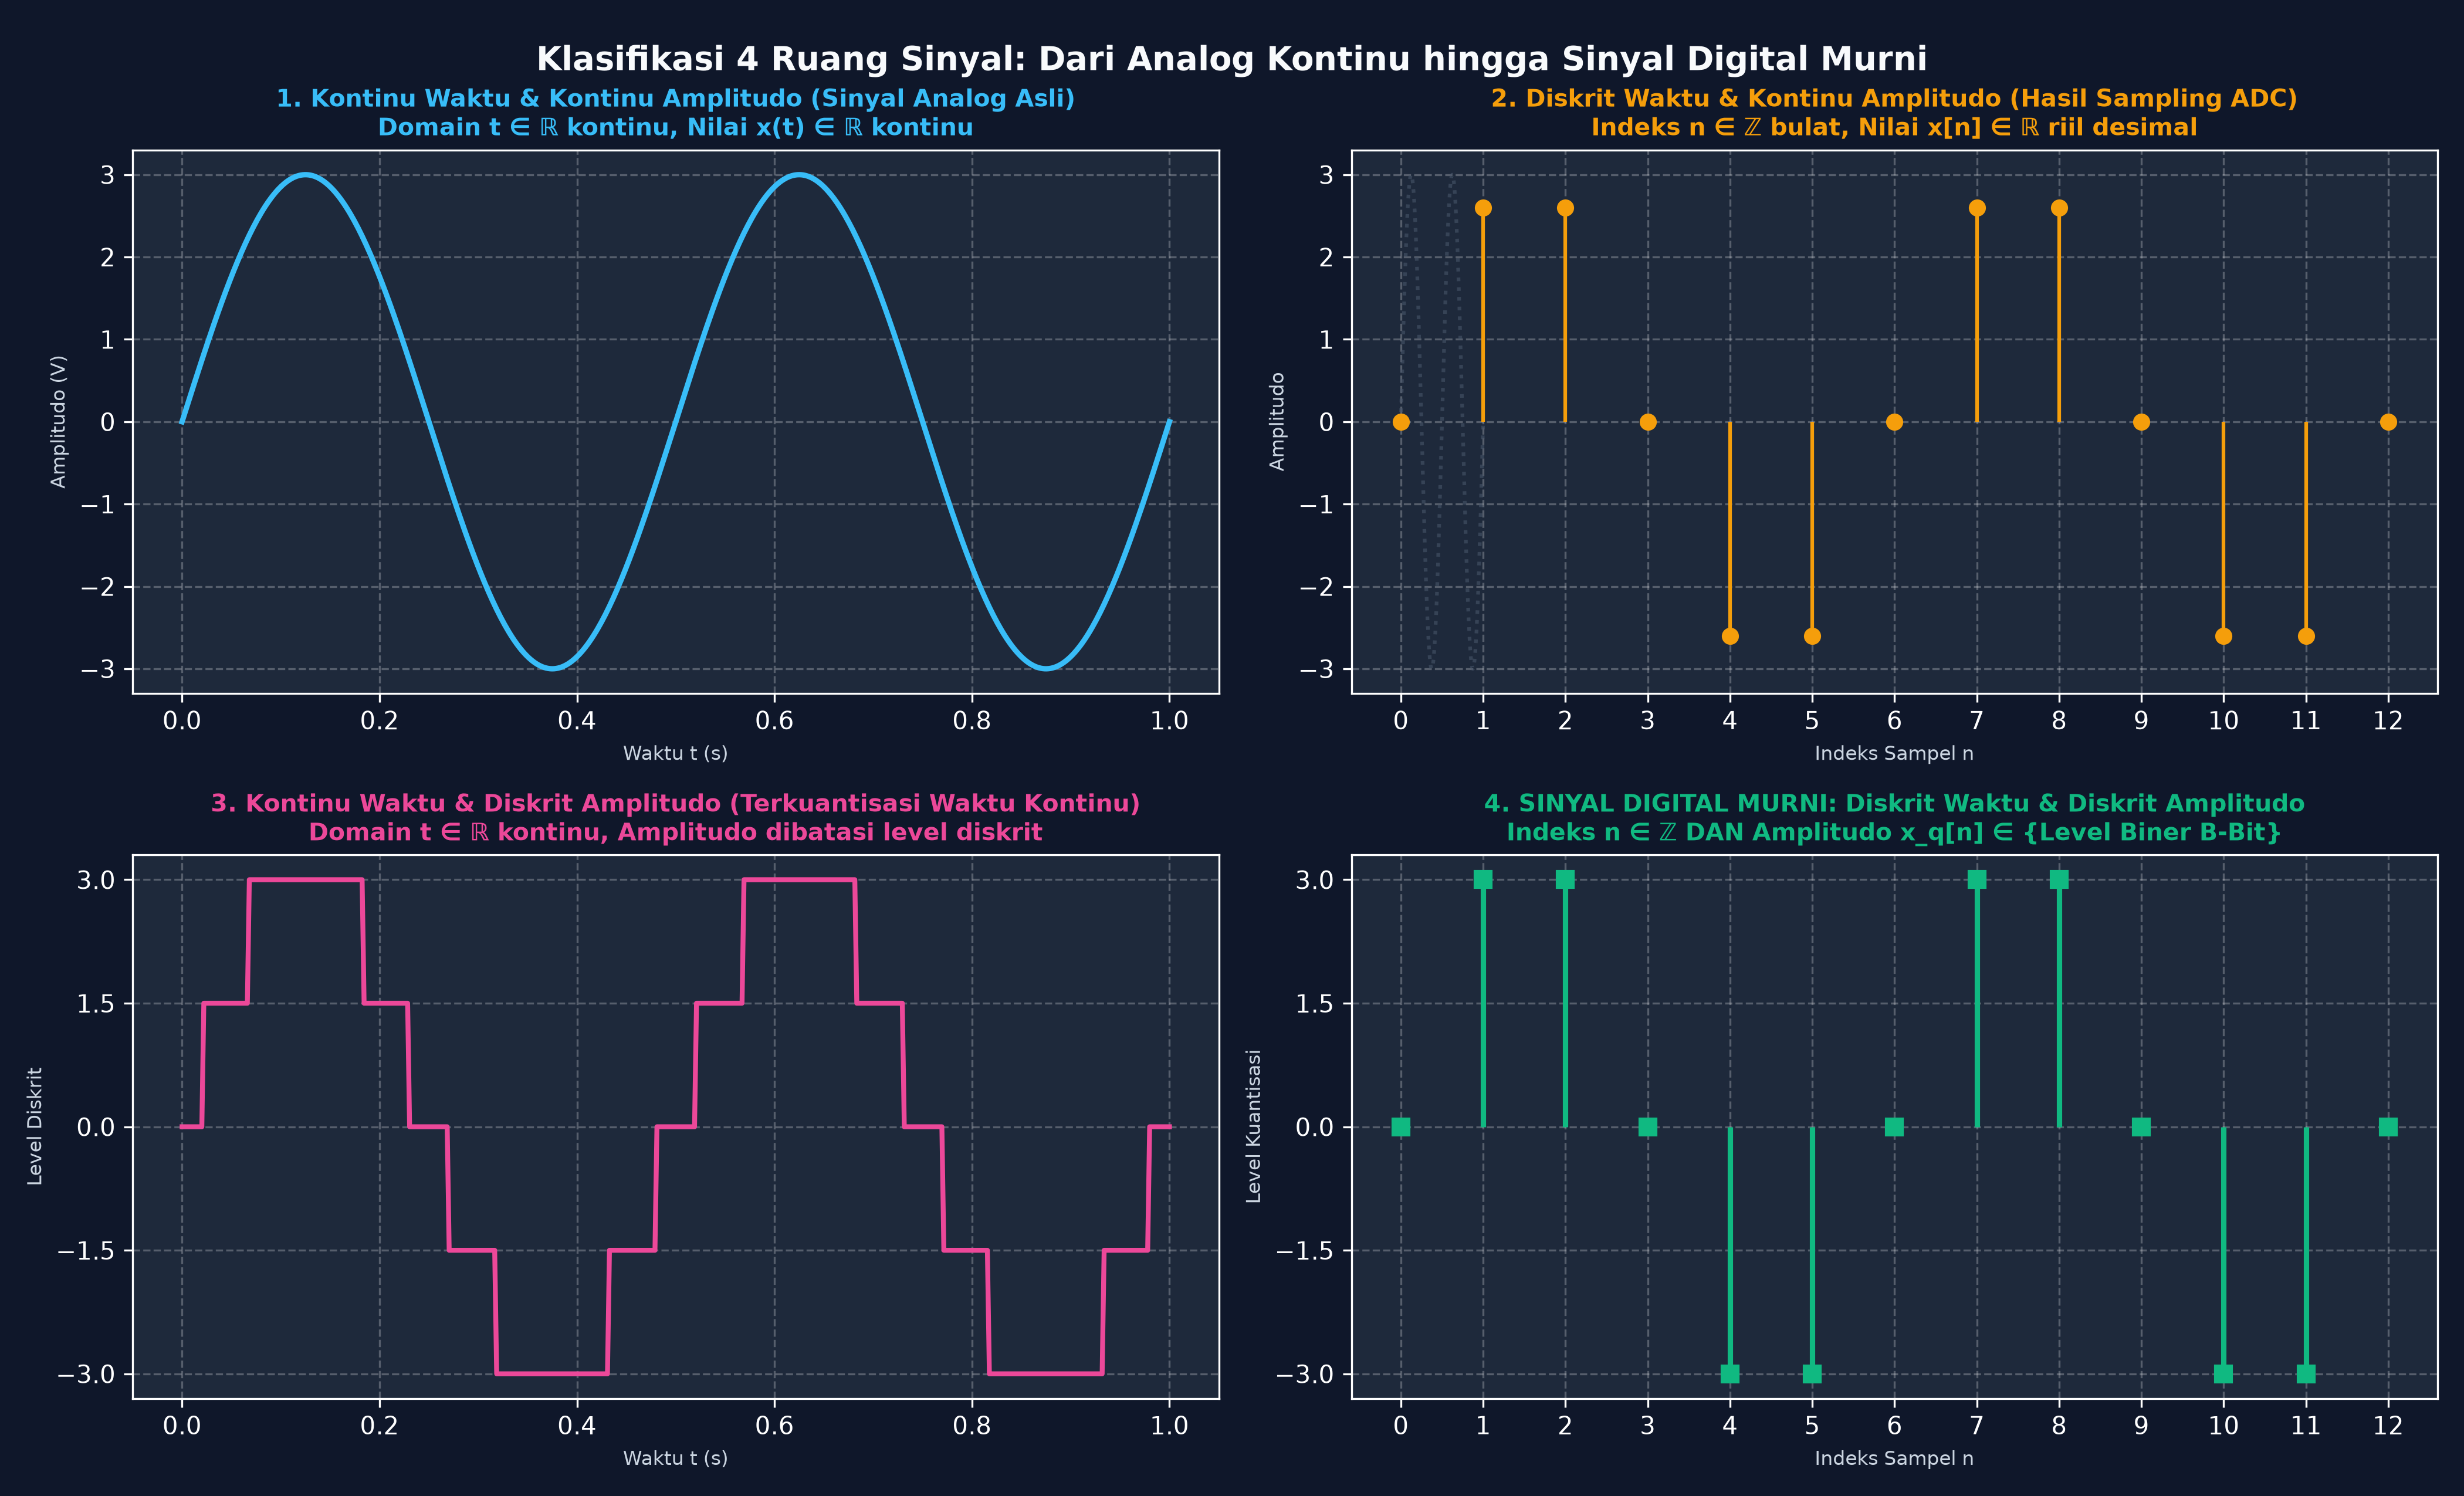
\includegraphics[width=0.92\linewidth]{assets/sinyal_digital_4_kuadran.png}
  \captionof{figure}{Klasifikasi 4 Ruang Sinyal fundamental berdasarkan kombinasi topologi waktu dan nilai amplitudo.}
\end{center}

\begin{analisisbox}[Dekomposisi 4 Kuadran Ruang Keadaan Sinyal]
\begin{enumerate}[leftmargin=*]
  \item \textbf{Kuadran 1 (Waktu Kontinu, Nilai Kontinu — Sinyal Analog Asli):} $x(t) \in \mathbb{R}, \forall t \in \mathbb{R}$. Contoh: tegangan langsung pada elektroda sensor bio-potensial EKG.
  \item \textbf{Kuadran 2 (Waktu Diskrit, Nilai Kontinu — Sinyal Sampled-Data):} $x[n] \in \mathbb{R}, \forall n \in \mathbb{Z}$. Tegangan tersimpan pada kapasitor rangkaian *Sample-and-Hold* sebelum masuk ke komparator ADC.
  \item \textbf{Kuadran 3 (Waktu Kontinu, Nilai Diskrit — Sinyal Terkuantisasi Analog):} $x_q(t) \in \mathbb{D}_L, \forall t \in \mathbb{R}$. Contoh: keluaran sistem transmisi pulsa modulasi *Pulse-Code* analog terkuantisasi sebelum clocking.
  \item \textbf{Kuadran 4 (Waktu Diskrit, Nilai Diskrit — SINYAL DIGITAL MURNI):} $x_q[n] \in \mathbb{D}_L, \forall n \in \mathbb{Z}$. Inilah satu-satunya format sinyal yang dapat dimanipulasi oleh memori RAM, register biner, dan arsitektur aritmatika ALU prosesor digital!
\end{enumerate}
\end{analisisbox}

\newpage
\subsection{Sinyal Deterministik vs Sinyal Acak (Random / Stokastik)}

\begin{center}
  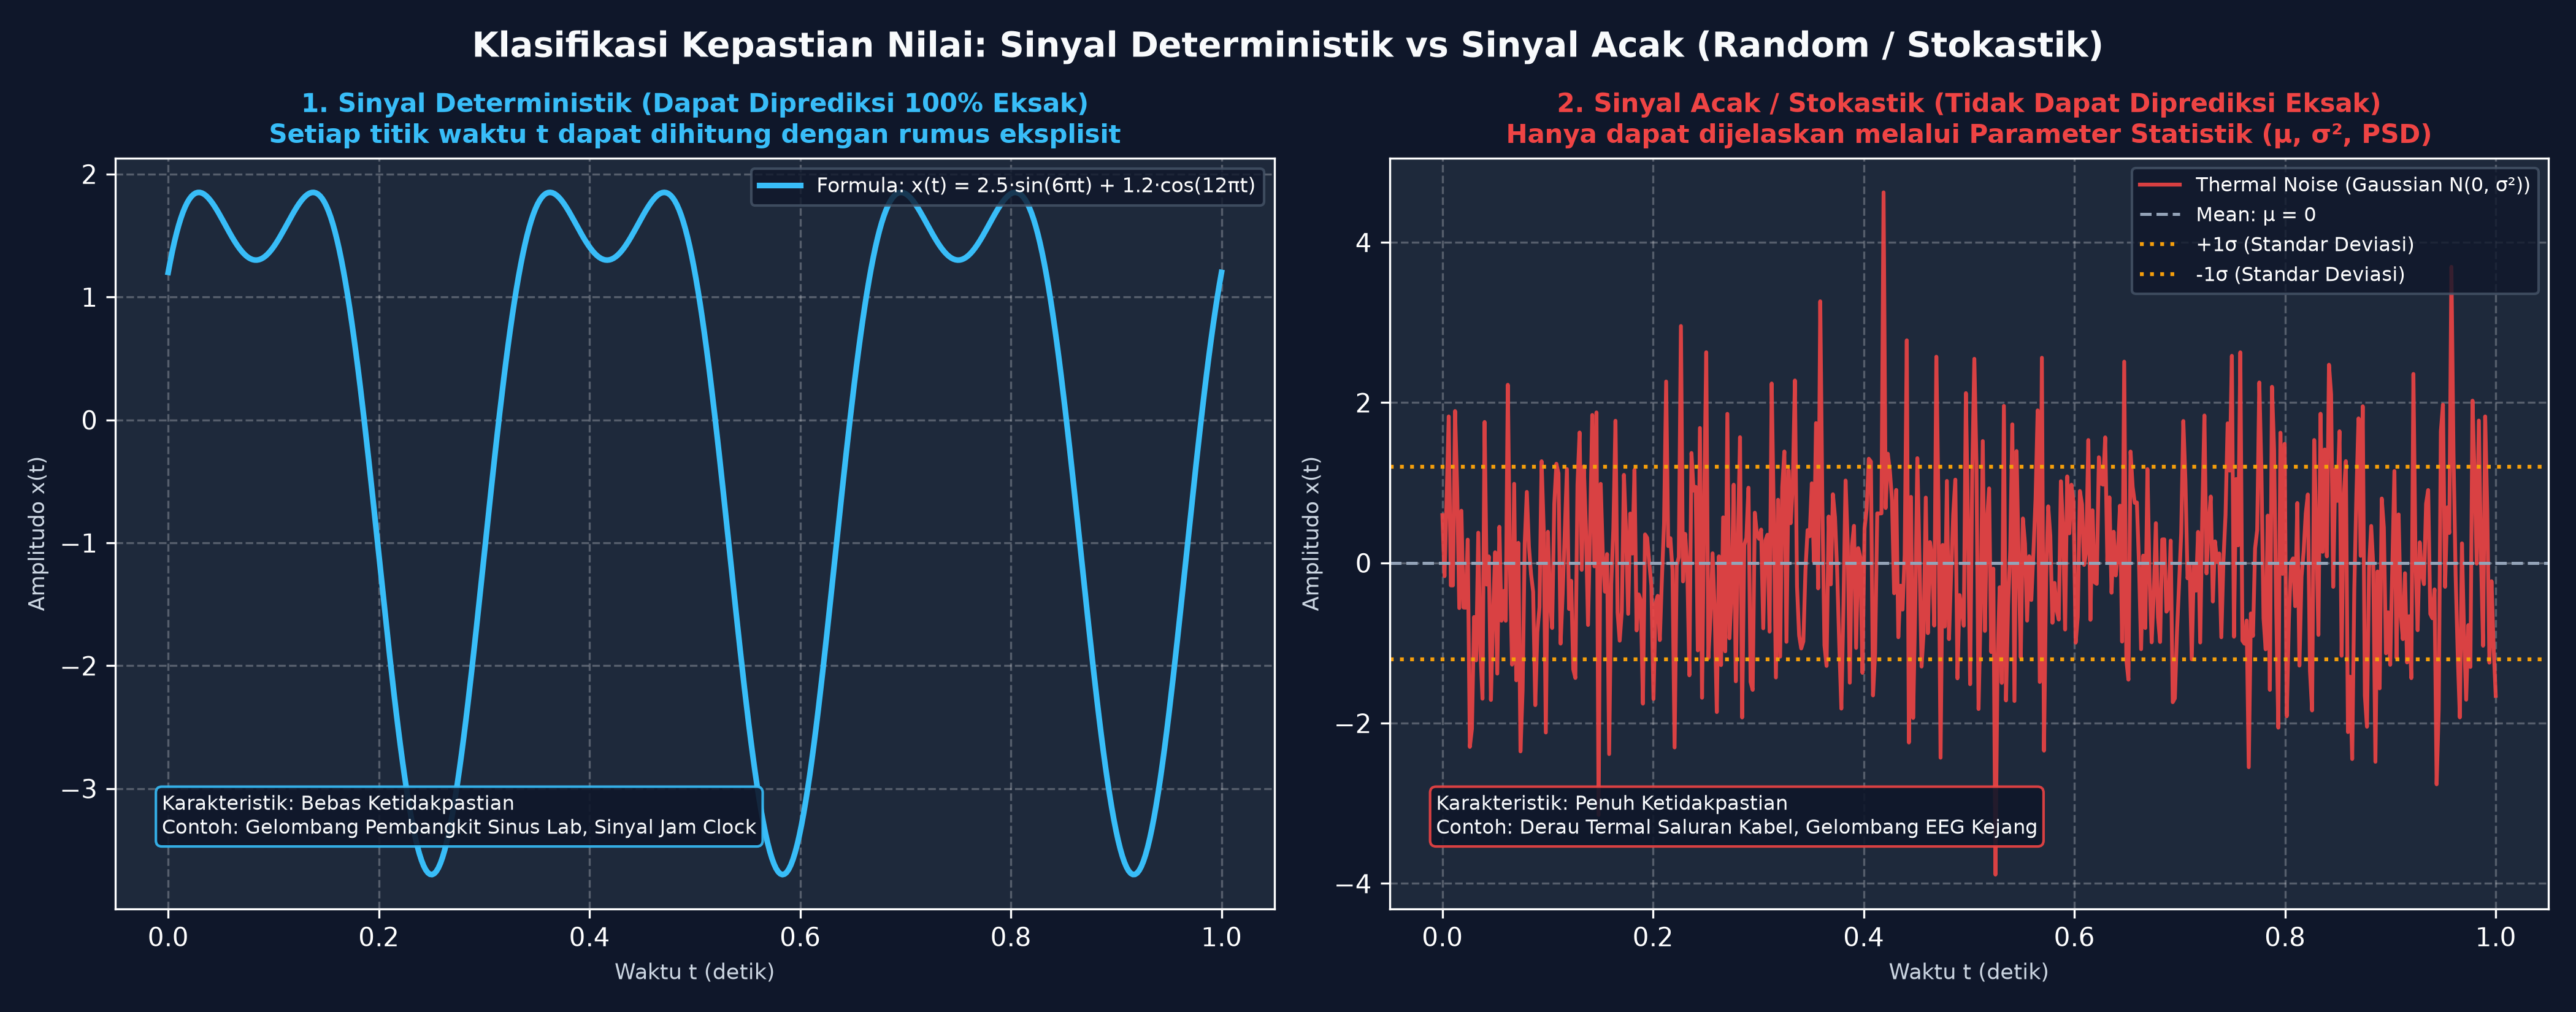
\includegraphics[width=0.95\linewidth]{assets/sinyal_deterministik_vs_acak.png}
  \captionof{figure}{Perbandingan sifat analitis sinyal Deterministik (matematis eksak) versus Sinyal Acak / Stokastik (probabilistik).}
\end{center}

\begin{analisisbox}[Analisis Stokastik: Fungsi Korelasi \& Teorema Wiener-Khinchin]
\begin{itemize}[leftmargin=*]
  \item \textbf{Sinyal Deterministik (Panel 1 — Biru Muda):}  
  Sinyal yang setiap nilai masa lalunya, saat ini, dan masa depannya dapat ditentukan \textbf{secara pasti 100\% tanpa ambiguitas} melalui hubungan analitik eksplisit, misalnya kombinasi deret Fourier:
  \begin{equation}
  x(t) = 2.5 \sin(6\pi t) + 1.2 \cos(12\pi t)
  \end{equation}
  Nilai $x(0.5\text{ s}) = 2.5 \sin(3\pi) + 1.2 \cos(6\pi) = 0 + 1.2(1) = 1.200\text{ V}$ dapat dihitung secara analitis presisi.

  \item \textbf{Sinyal Acak / Stokastik (Panel 2 — Merah):}  
  Sinyal yang masa depannya tidak dapat diprediksi secara eksak dan hanya dapat dimodelkan sebagai proses acak (*stochastic process*) $X(t, \zeta)$ melalui parameter statistik ensemble:
  \begin{enumerate}
    \item \textbf{Nilai Ekspektasi / Mean ($\mu_x(t)$):} $\mu_x(t) = \mathbb{E}[X(t)] = \int_{-\infty}^{\infty} x f_X(x; t) dx$.
    \item \textbf{Fungsi Autokorelasi ($R_{xx}(t_1, t_2)$):} $R_{xx}(t_1, t_2) = \mathbb{E}[X(t_1) X^*(t_2)]$.
    \item \textbf{Stasioneritas Lebar (Wide-Sense Stationary / WSS):} Jika $\mu_x(t) = \mu_x$ (konstan) dan $R_{xx}(t_1, t_2) = R_{xx}(\tau)$ di mana $\tau = t_1 - t_2$.
  \end{enumerate}
  \textbf{Teorema Wiener-Khinchin:} Kerapatan spektral daya (*Power Spectral Density* / PSD) dari sinyal acak WSS adalah Transformasi Fourier dari fungsi autokorelasinya:
  \begin{equation}
  S_{xx}(F) = \mathcal{F}\left\{ R_{xx}(\tau) \right\} = \int_{-\infty}^{\infty} R_{xx}(\tau) e^{-j 2\pi F \tau} d\tau
  \end{equation}
  Untuk derau putih murni (*Additive White Gaussian Noise* / AWGN), autokorelasinya berupa impuls $R_{ww}(\tau) = \sigma^2 \delta(\tau)$, menghasilkan spektrum frekuensi yang datar rata di semua frekuensi: $S_{ww}(F) = \sigma^2\ [\text{W/Hz}]$.
\end{itemize}
\end{analisisbox}

% =========================================================================
\section{Analisis Frekuensi \& Gelombang Sinusoidal (Kontinu vs Diskrit)}
% =========================================================================

\subsection{Perbandingan Domain Frekuensi: Sinyal Waktu Kontinu vs Sinyal Waktu Diskrit}

Pemetaan frekuensi dari domain kontinu ($F,\Omega$) ke domain diskrit ($f,\omega$) terjadi melalui hubungan parameter interval sampling $T_s = 1/F_s$:
\begin{equation}
\omega = \Omega T_s = \frac{\Omega}{F_s} = \frac{2\pi F}{F_s} = 2\pi f \quad [\text{rad/sampel}], \qquad f = \frac{F}{F_s} \quad [\text{siklus/sampel}]
\end{equation}

\begin{center}
  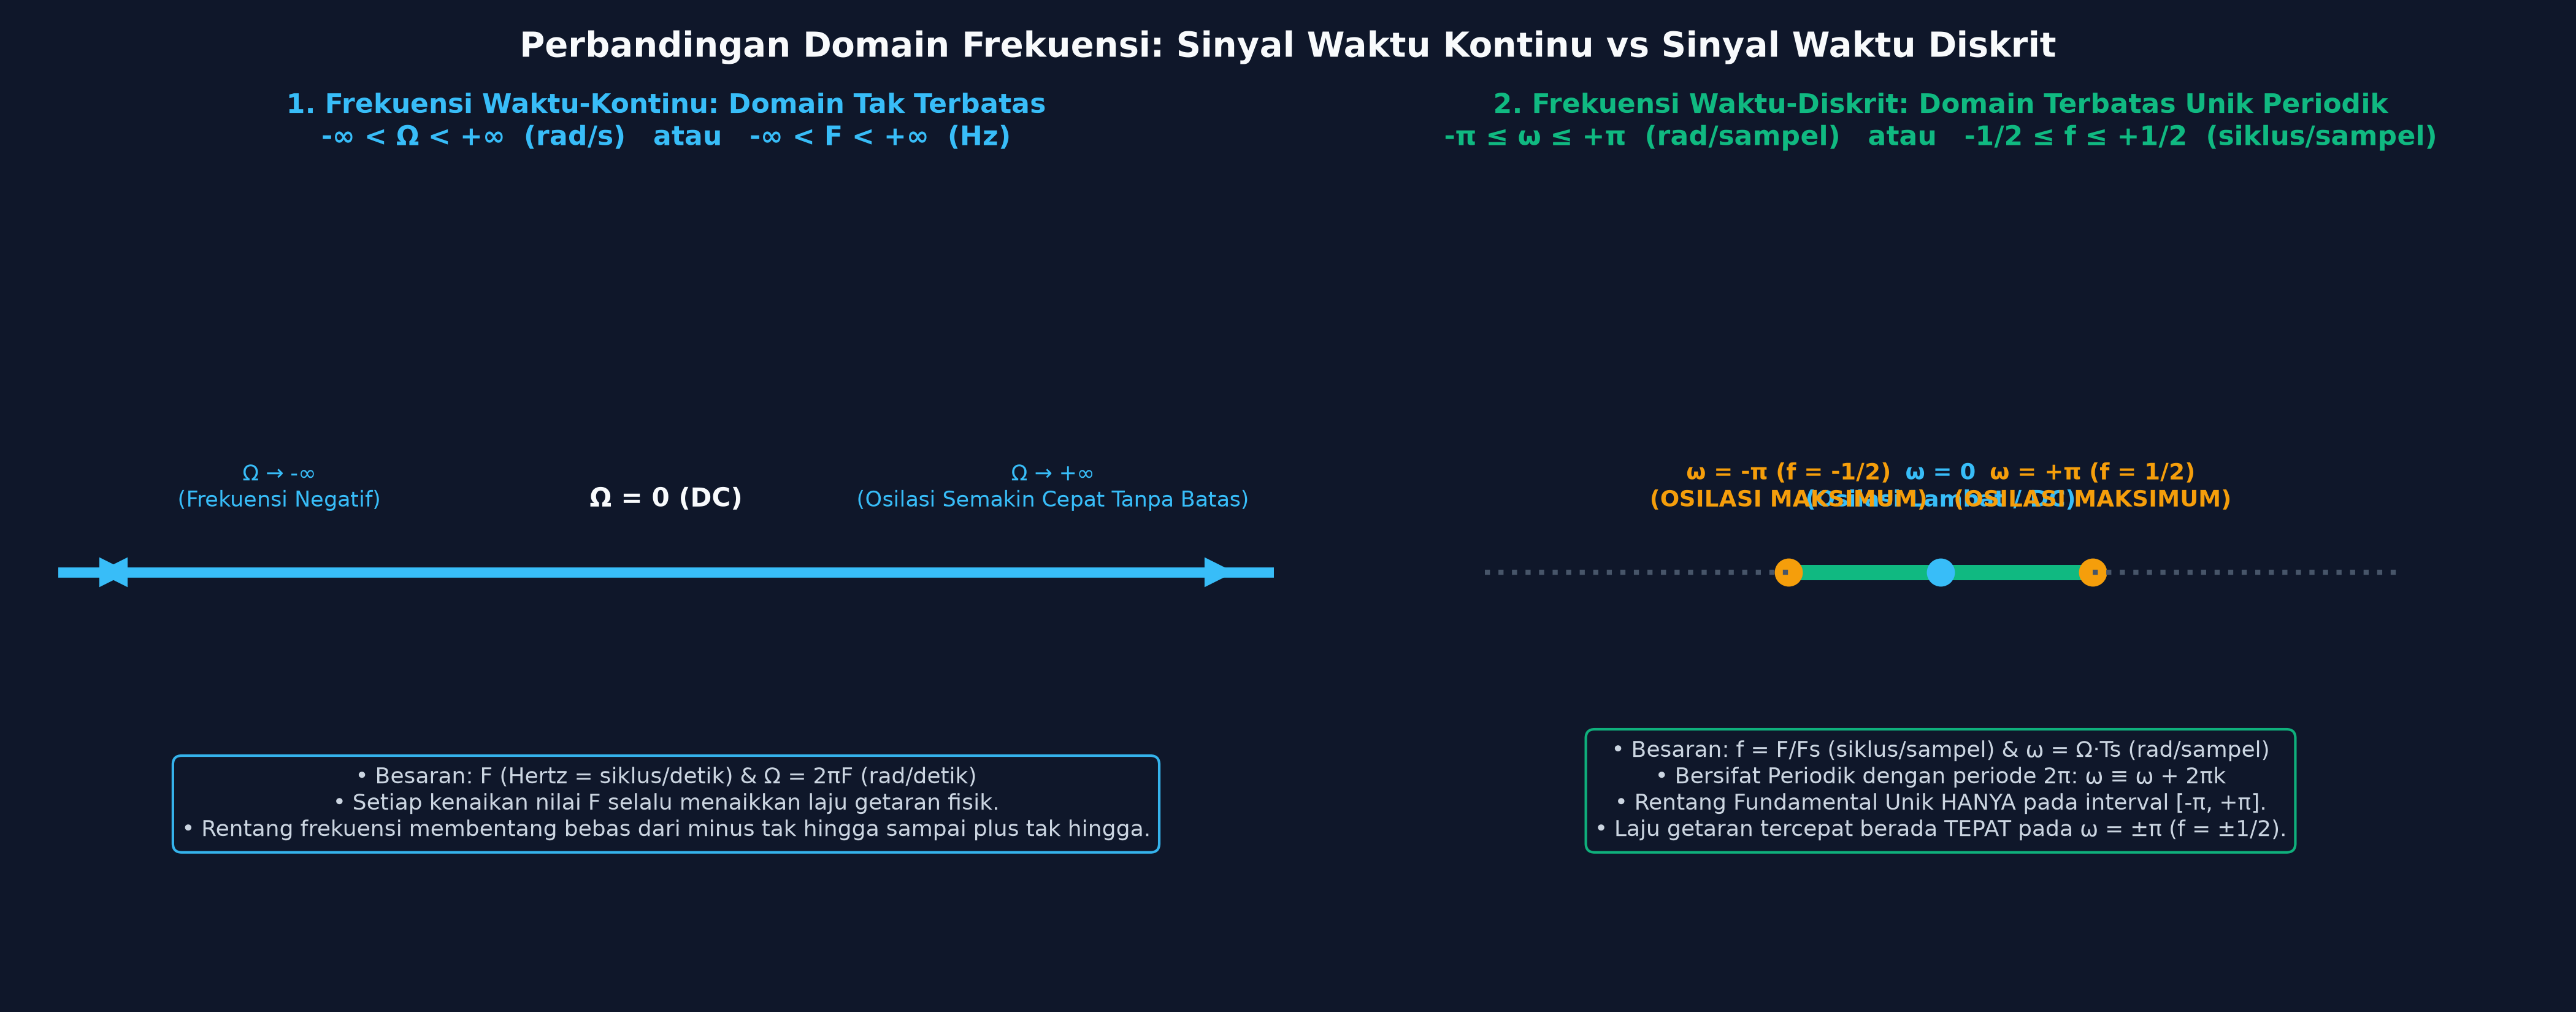
\includegraphics[width=0.95\linewidth]{assets/frekuensi_kontinu_vs_diskrit.png}
  \captionof{figure}{Pemetaan fundamental domain frekuensi fisik kontinu ($-\infty < \Omega < \infty$) ke dalam domain frekuensi diskrit terbatas periodik ($-\pi \leq \omega \leq \pi$).}
\end{center}

\begin{table}[h!]
\centering
\small
\caption{Tabel Perbandingan Komprehensif Domain Frekuensi Waktu-Kontinu vs Waktu-Diskrit}
\begin{tabularx}{\textwidth}{l>{\raggedright\arraybackslash}X>{\raggedright\arraybackslash}X}
\toprule
\textbf{Karakteristik Parameter} & \textbf{Domain Waktu-Kontinu (Analog)} & \textbf{Domain Waktu-Diskrit (Digital)} \\
\midrule
\textbf{Frekuensi Siklik} & $F$ ($\text{Hertz} = \text{siklus/detik}$) & $f = F / F_s$ ($\text{siklus/sampel}$) \\
\textbf{Frekuensi Sudut} & $\Omega = 2\pi F$ ($\text{rad/detik}$) & $\omega = \Omega T_s = 2\pi f$ ($\text{rad/sampel}$) \\
\textbf{Rentang Nilai Unik} & $-\infty < \Omega < +\infty$ (Tak terbatas) & $\mathbf{-\pi \leq \omega \leq +\pi}$ atau $\mathbf{-\frac{1}{2} \leq f \leq +\frac{1}{2}}$ \\
\textbf{Sifat Periodisitas Spektrum} & Bersifat Aperiodik pada sumbu $\Omega$ & \textbf{Periodik mutlak dengan periode $2\pi$} ($\omega \equiv \omega + 2\pi k$) \\
\textbf{Laju Osilasi Tertinggi} & $\Omega \to \infty$ (Meningkat tanpa batas) & \textbf{Tercapai tepat di $\omega = \pm \pi$ ($f = \pm 1/2$)} \\
\textbf{Representasi Transformasi} & Fourier Transform: $X(j\Omega) = \int x(t)e^{-j\Omega t}dt$ & DTFT: $X(e^{j\omega}) = \sum x[n] e^{-j\omega n}$ \\
\bottomrule
\end{tabularx}
\end{table}

\newpage
\subsection{Sinyal Sinusoidal Waktu-Kontinu: Keunikan Frekuensi Fisik \& Laju Tak Terbatas}

Persamaan gelombang sinusoidal waktu-kontinu dinyatakan sebagai $x_a(t) = A \cos(\Omega t + \theta) = A \cos(2\pi F t + \theta)$.

\begin{center}
  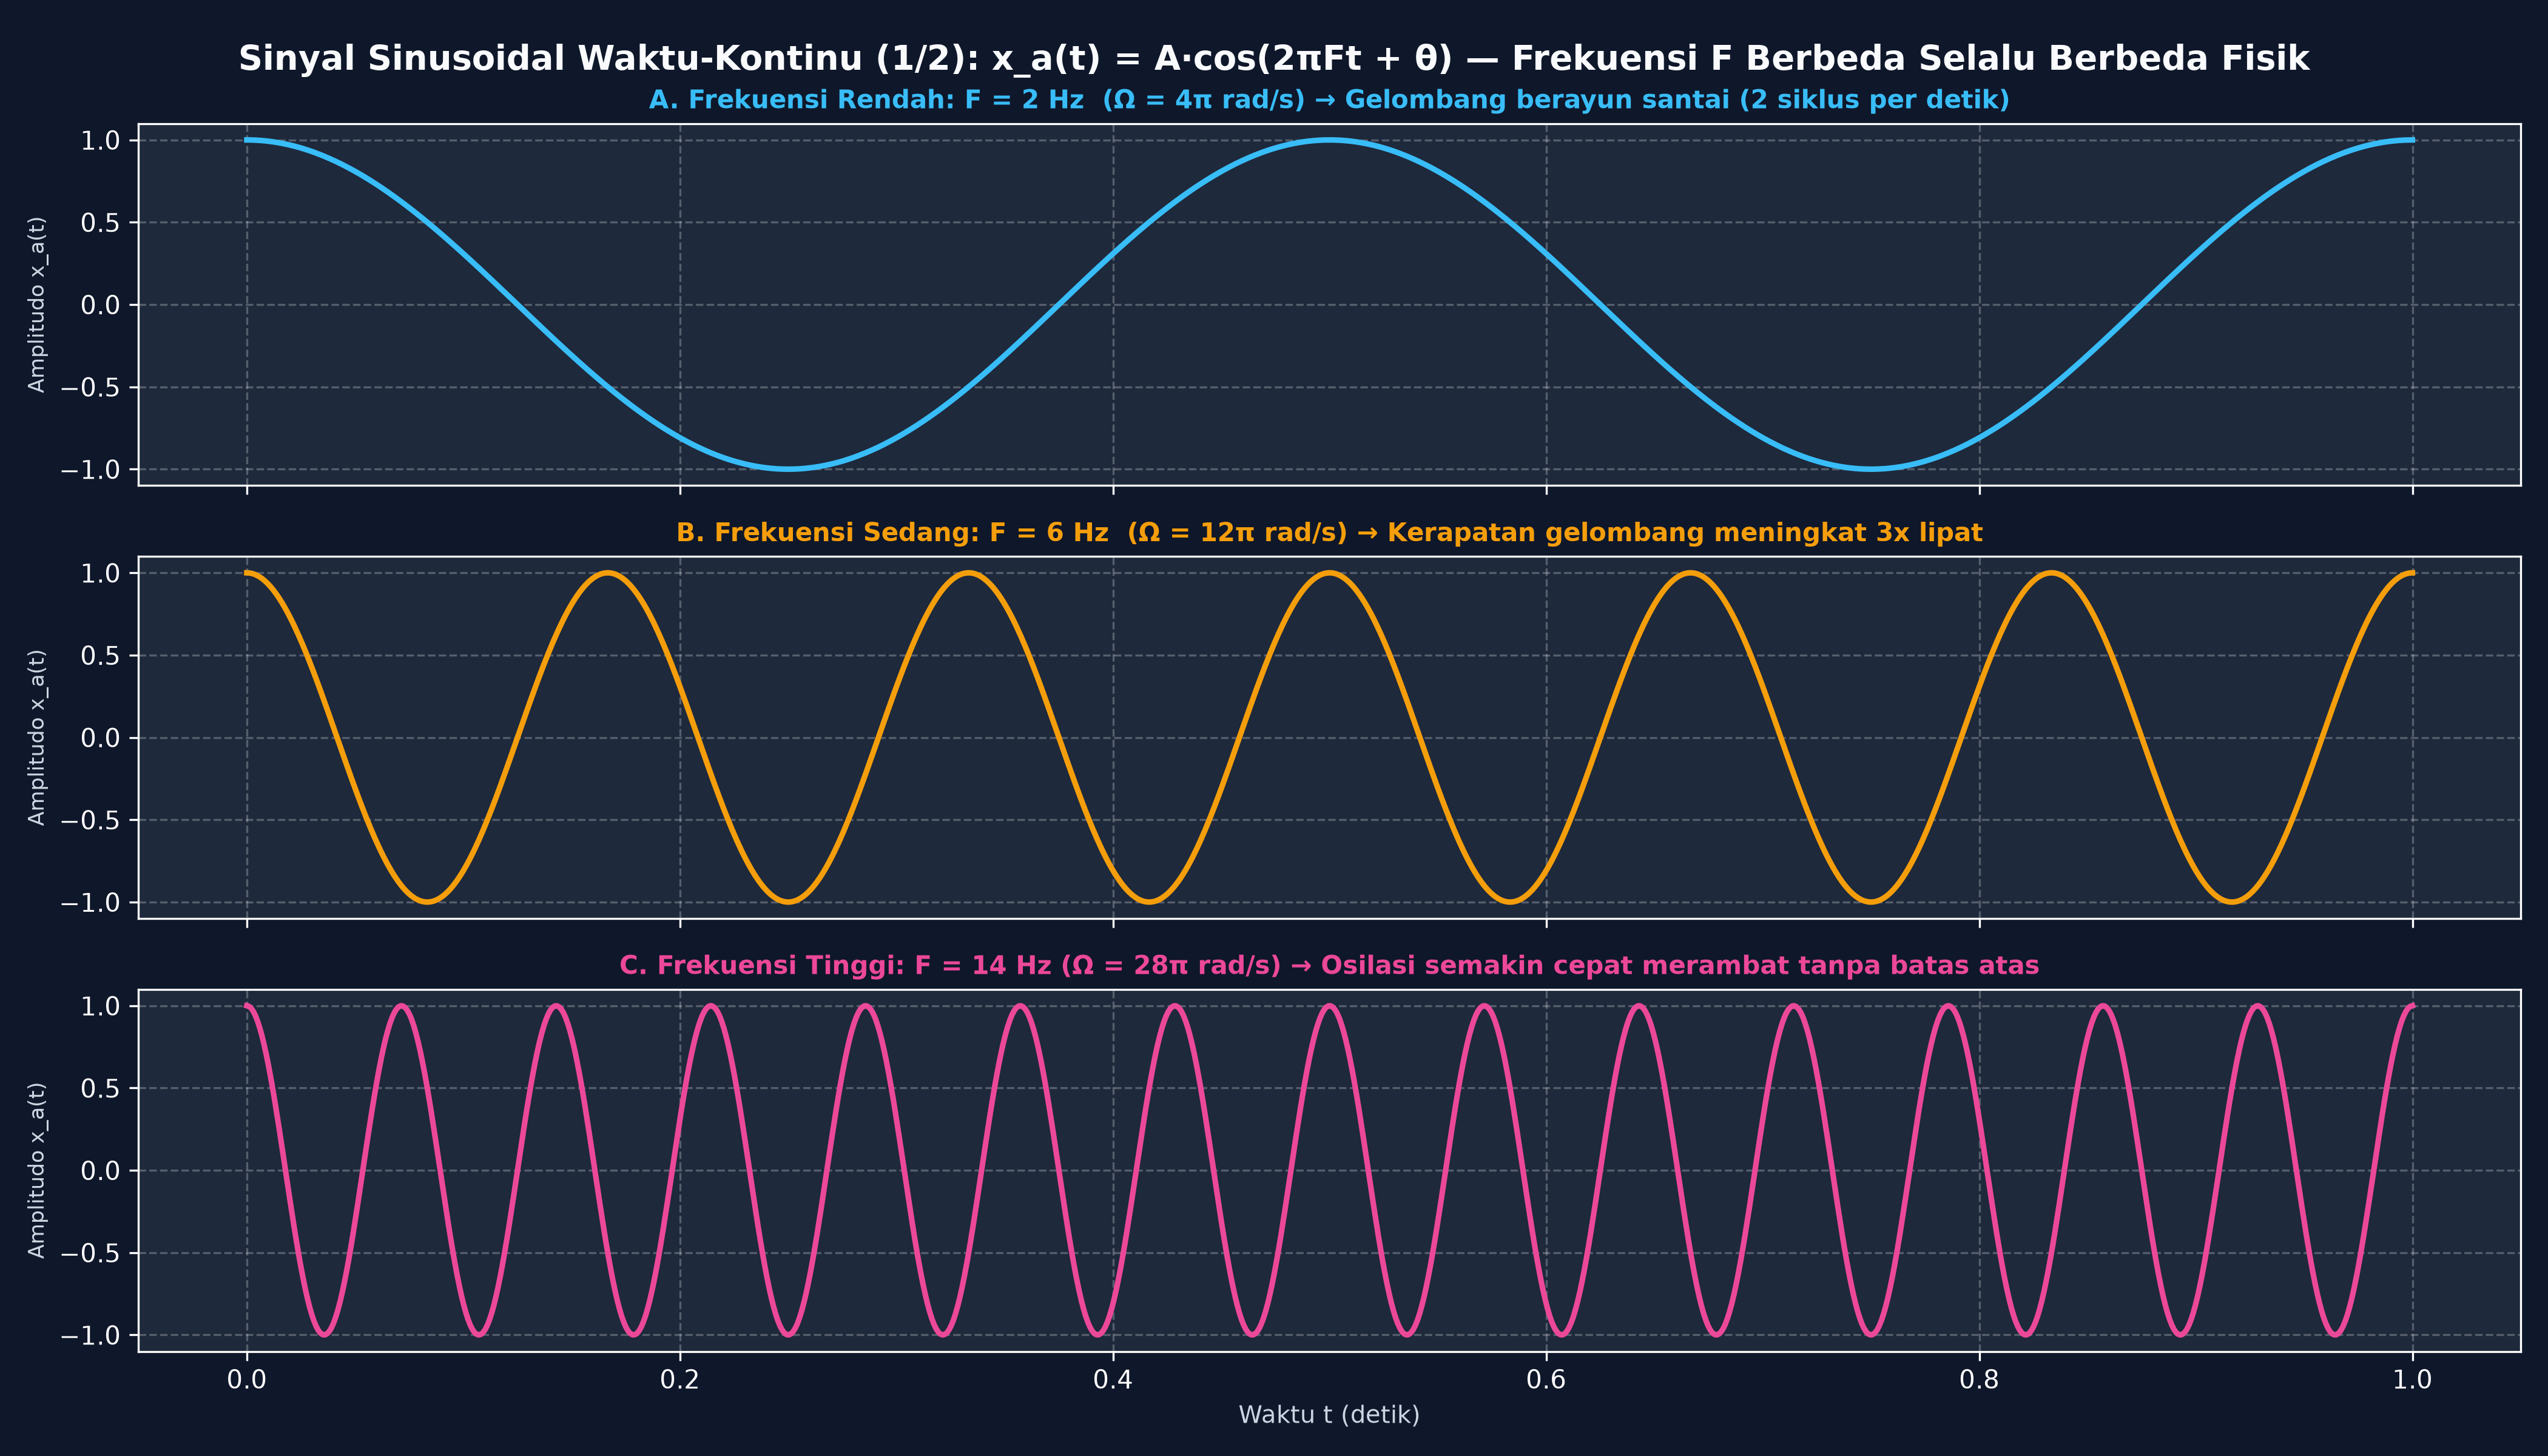
\includegraphics[width=0.92\linewidth]{assets/sinus_kontinu_karakteristik_1.png}
  \captionof{figure}{Sifat Sinus Kontinu (1/2): Setiap perbedaan frekuensi $F$ menghasilkan gelombang fisik unik yang berosilasi semakin cepat tanpa batas atas.}
\end{center}

\begin{analisisbox}[Pembuktian Keunikan \& Laju Tak Terbatas]
\begin{enumerate}[leftmargin=*]
  \item \textbf{Keunikan Frekuensi Fisik (Ortogonalitas Continuous Basis):}  
  Dua sinyal sinusoidal kontinu dengan frekuensi berbeda $F_1 \neq F_2$ selalu independen secara ortogonal pada interval pengamatan kelipatan persekutuan $T_0$:
  \begin{equation}
  \frac{1}{T_0}\int_0^{T_0} \cos(2\pi F_1 t) \cos(2\pi F_2 t) dt = \frac{1}{2} \delta_{F_1, F_2}
  \end{equation}
  Tidak ada dua frekuensi kontinu berbeda yang dapat menghasilkan profil fisik gelombang yang sama.

  \item \textbf{Laju Osilasi Bertambah Monotonik Menuju Tak Hingga:}  
  Turunan pertama sinyal terhadap waktu merepresentasikan laju perubahan tegangan:
  \begin{equation}
  \left| \frac{d x_a(t)}{dt} \right|_{\max} = | -A \cdot 2\pi F \sin(2\pi F t + \theta) |_{\max} = 2\pi A F
  \end{equation}
  Ketika $F \to \infty$, laju kemiringan tegangan $\frac{dx_a}{dt} \to \infty$ bertambah tanpa ada batas maksimum.
\end{enumerate}
\end{analisisbox}

\vspace{0.3cm}
\subsection{Sinyal Sinusoidal Waktu-Kontinu: Periodisitas Universal}

\begin{center}
  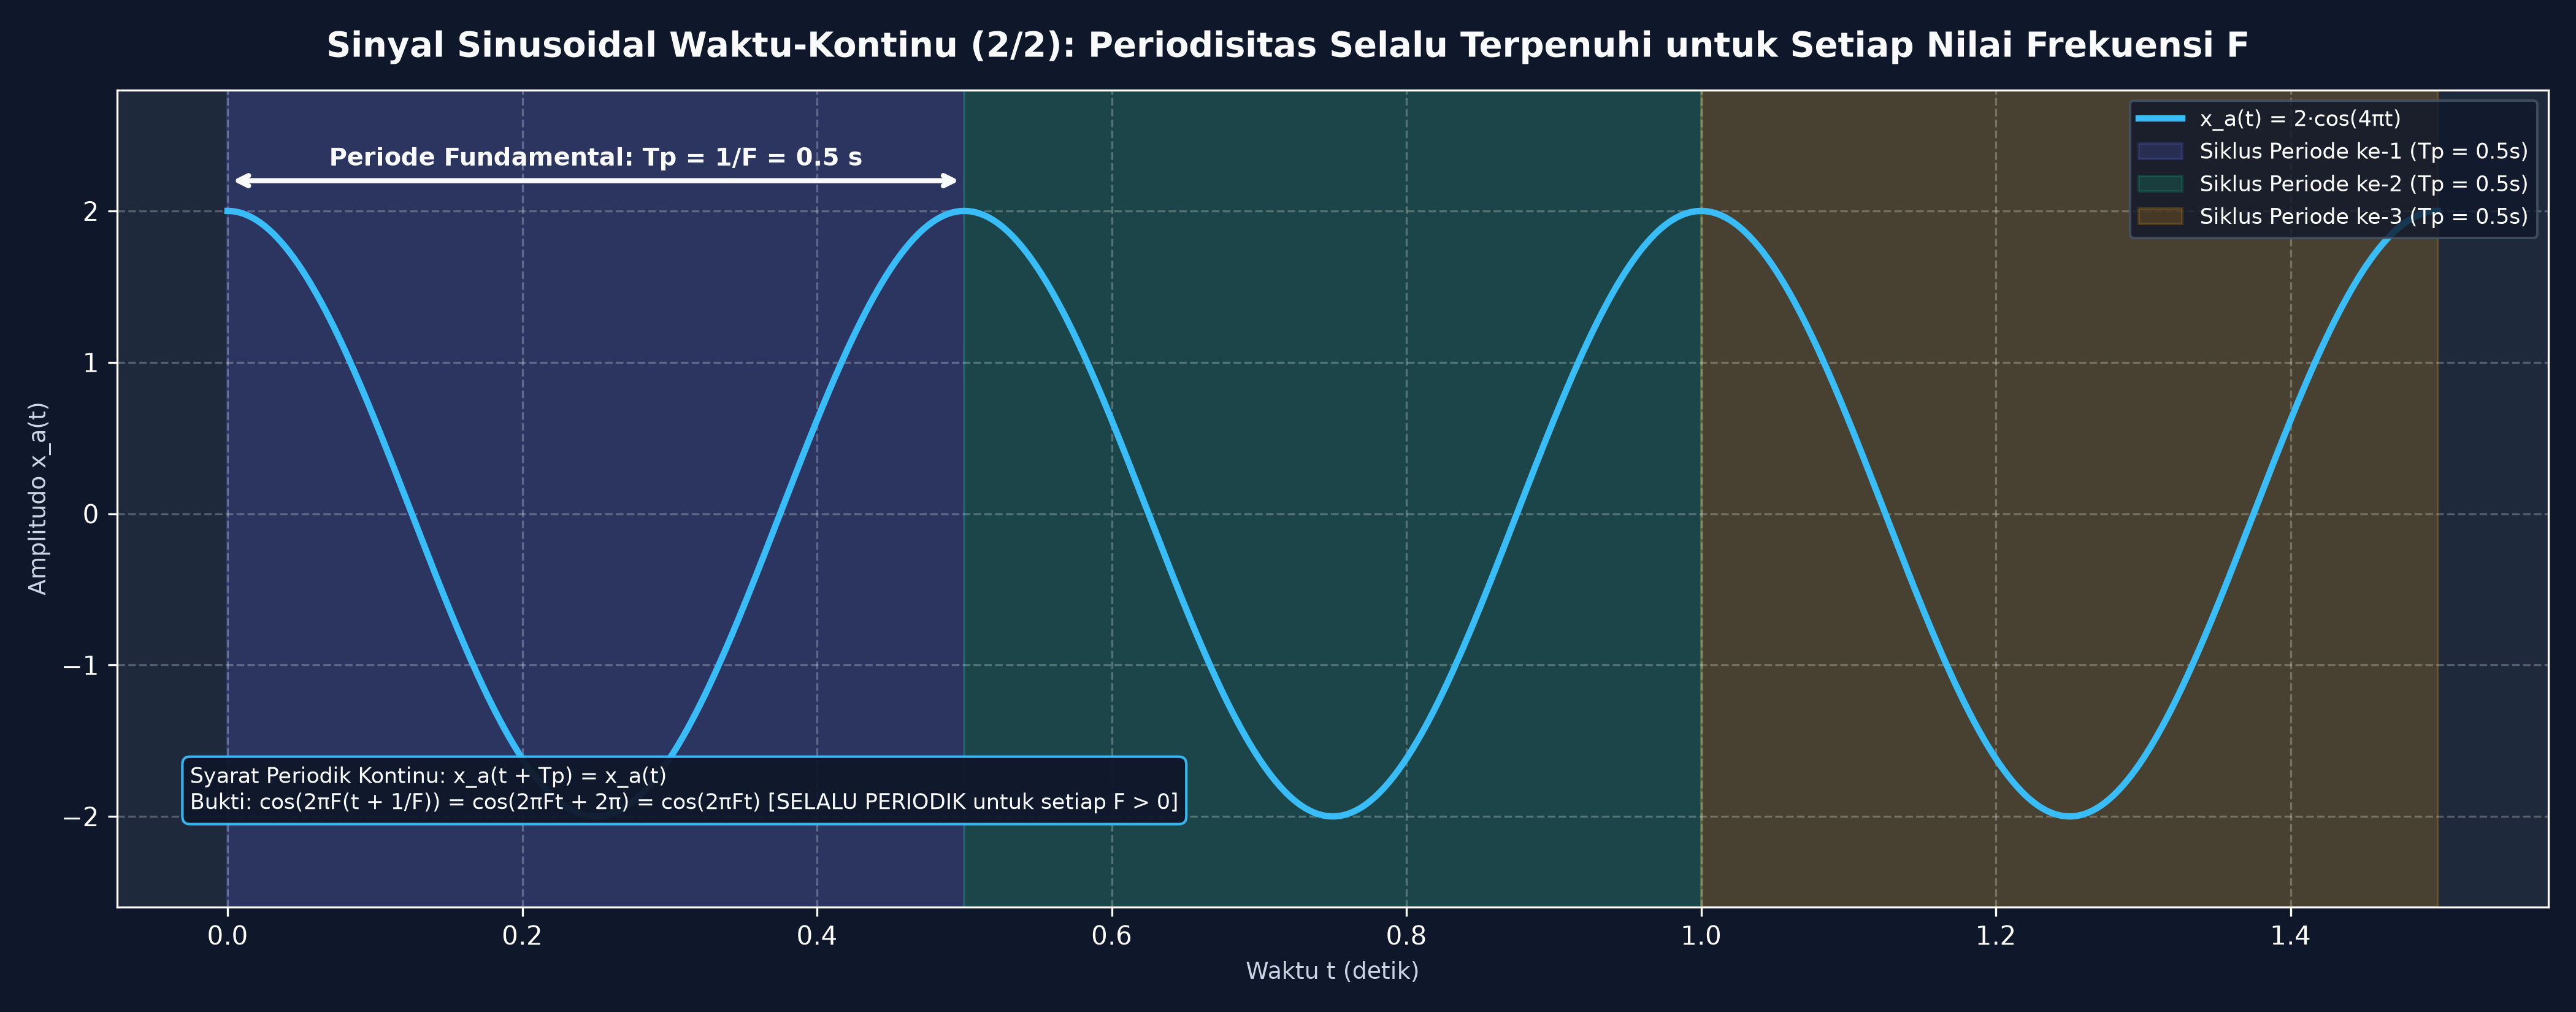
\includegraphics[width=0.92\linewidth]{assets/sinus_kontinu_periodisitas_2.png}
  \captionof{figure}{Sifat Sinus Kontinu (2/2): Sinyal kontinu SELALU periodik untuk setiap frekuensi $F > 0$ dengan $T_p = 1/F$.}
\end{center}

\begin{analisisbox}[Pembuktian Matematis Periodisitas Universal Sinyal Kontinu]
Suatu sinyal $x_a(t)$ dikatakan periodik jika terdapat konstanta waktu $T_p > 0$ sedemikian rupa sehingga $x_a(t + T_p) = x_a(t), \forall t \in \mathbb{R}$. Untuk sembarang frekuensi $F > 0$:
\begin{equation}
x_a(t + T_p) = A \cos\left(2\pi F \left(t + \frac{1}{F}\right) + \theta\right) = A \cos(2\pi F t + 2\pi + \theta) = A \cos(2\pi F t + \theta) = x_a(t)
\end{equation}
Karena kesamaan ini berlaku identik untuk semua $F \in \mathbb{R}^+$, maka **semua sinyal sinusoidal kontinu di alam semesta dijamin 100\% selalu periodik**.
\end{analisisbox}

\newpage
\subsection{Sinyal Sinusoidal Waktu-Diskrit: Syarat Wajib Periodisitas Bilangan Rasional}

Persamaan umum sinusoidal diskrit: $x[n] = A \cos(\omega n + \theta) = A \cos(2\pi f n + \theta)$.

\begin{teoremabox}[Fakta Krusial: Sinyal Sinus Diskrit TIDAK SELALU Periodik!]
Agar sinyal diskrit $x[n]$ periodik dengan periode fundamental integer $N \in \mathbb{Z}^+$ ($x[n + N] = x[n]$), maka frekuensi sikliknya $f$ wajib berupa \textbf{Bilangan Rasional}:
\begin{equation}
\cos(2\pi f (n + N) + \theta) = \cos(2\pi f n + 2\pi f N + \theta) \equiv \cos(2\pi f n + 2\pi k + \theta)
\end{equation}
\begin{equation}
\implies 2\pi f N = 2\pi k \implies \mathbf{f = \frac{k}{N} \in \mathbb{Q}, \quad k, N \in \mathbb{Z}^+}
\end{equation}
Periode fundamental integer terkecil sampel $N$ dihitung melalui:
\begin{equation}
N = \frac{k}{f} = \frac{2\pi k}{\omega}, \quad \text{di mana } k \text{ adalah integer terkecil pembuat } N \in \mathbb{Z}^+
\end{equation}
\end{teoremabox}

\begin{center}
  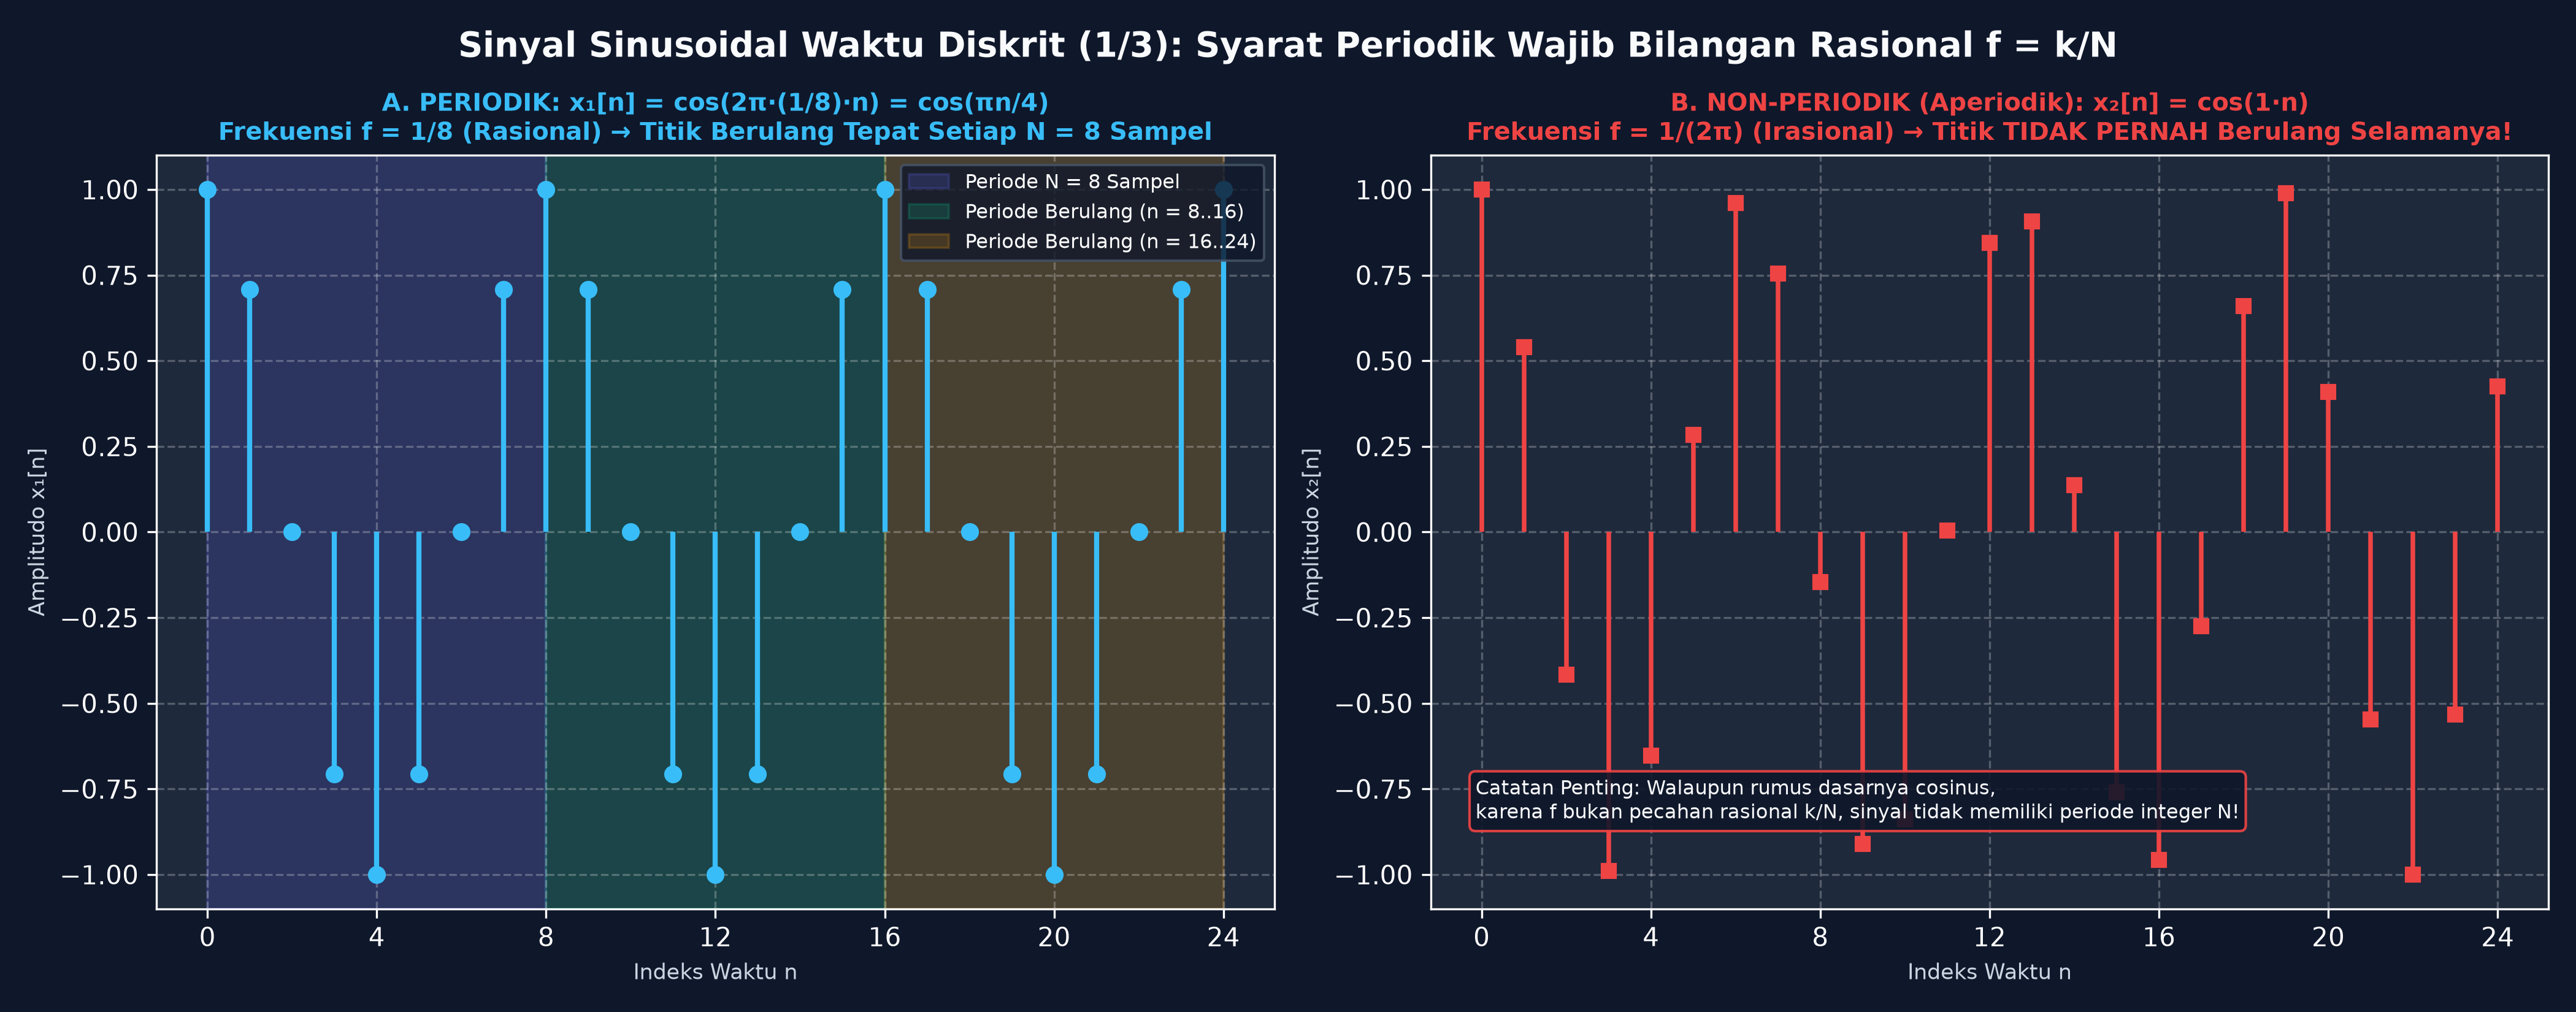
\includegraphics[width=0.92\linewidth]{assets/sinus_diskrit_periodisitas_1.png}
  \captionof{figure}{Komparasi: Panel A Periodik ($f = 1/8 \in \mathbb{Q}, N = 8$) vs Panel B Aperiodik ($f = 1/(2\pi) \notin \mathbb{Q}$, titik sampel tidak pernah berulang).}
\end{center}

\begin{analisisbox}[Pembuktian Analitik Panel A vs Panel B]
\begin{itemize}[leftmargin=*]
  \item \textbf{Panel A ($x_1[n] = \cos(\frac{\pi}{4} n)$):} $\omega = \frac{\pi}{4} \implies f = \frac{\omega}{2\pi} = \frac{\pi/4}{2\pi} = \frac{1}{8}$. Karena $\frac{1}{8} \in \mathbb{Q}$ (bilangan rasional), sinyal **Periodik** dengan periode $N = \frac{1}{1/8} = 8\text{ sampel}$. Pola sampel berulang identik setiap 8 ketukan.
  \item \textbf{Panel B ($x_2[n] = \cos(1 \cdot n)$):} $\omega = 1\text{ rad/sampel} \implies f = \frac{1}{2\pi}$. Karena $\pi$ adalah bilangan transendental irasional, maka $f \notin \mathbb{Q}$. Tidak ada bilangan bulat $N$ dan $k$ yang memenuhi $N = 2\pi k$. Akibatnya, sinyal $x_2[n]$ **100\% Aperiodik / Non-Periodik**; titik-titik sampelnya tidak akan pernah berulang sama persis di sepanjang garis waktu sampai kapan pun!
\end{itemize}
\end{analisisbox}

\vspace{0.3cm}
\subsection{Sinyal Sinusoidal Waktu-Diskrit: Fenomena Frekuensi Identik Kelipatan \texorpdfstring{$2\pi$}{2pi}}

\begin{center}
  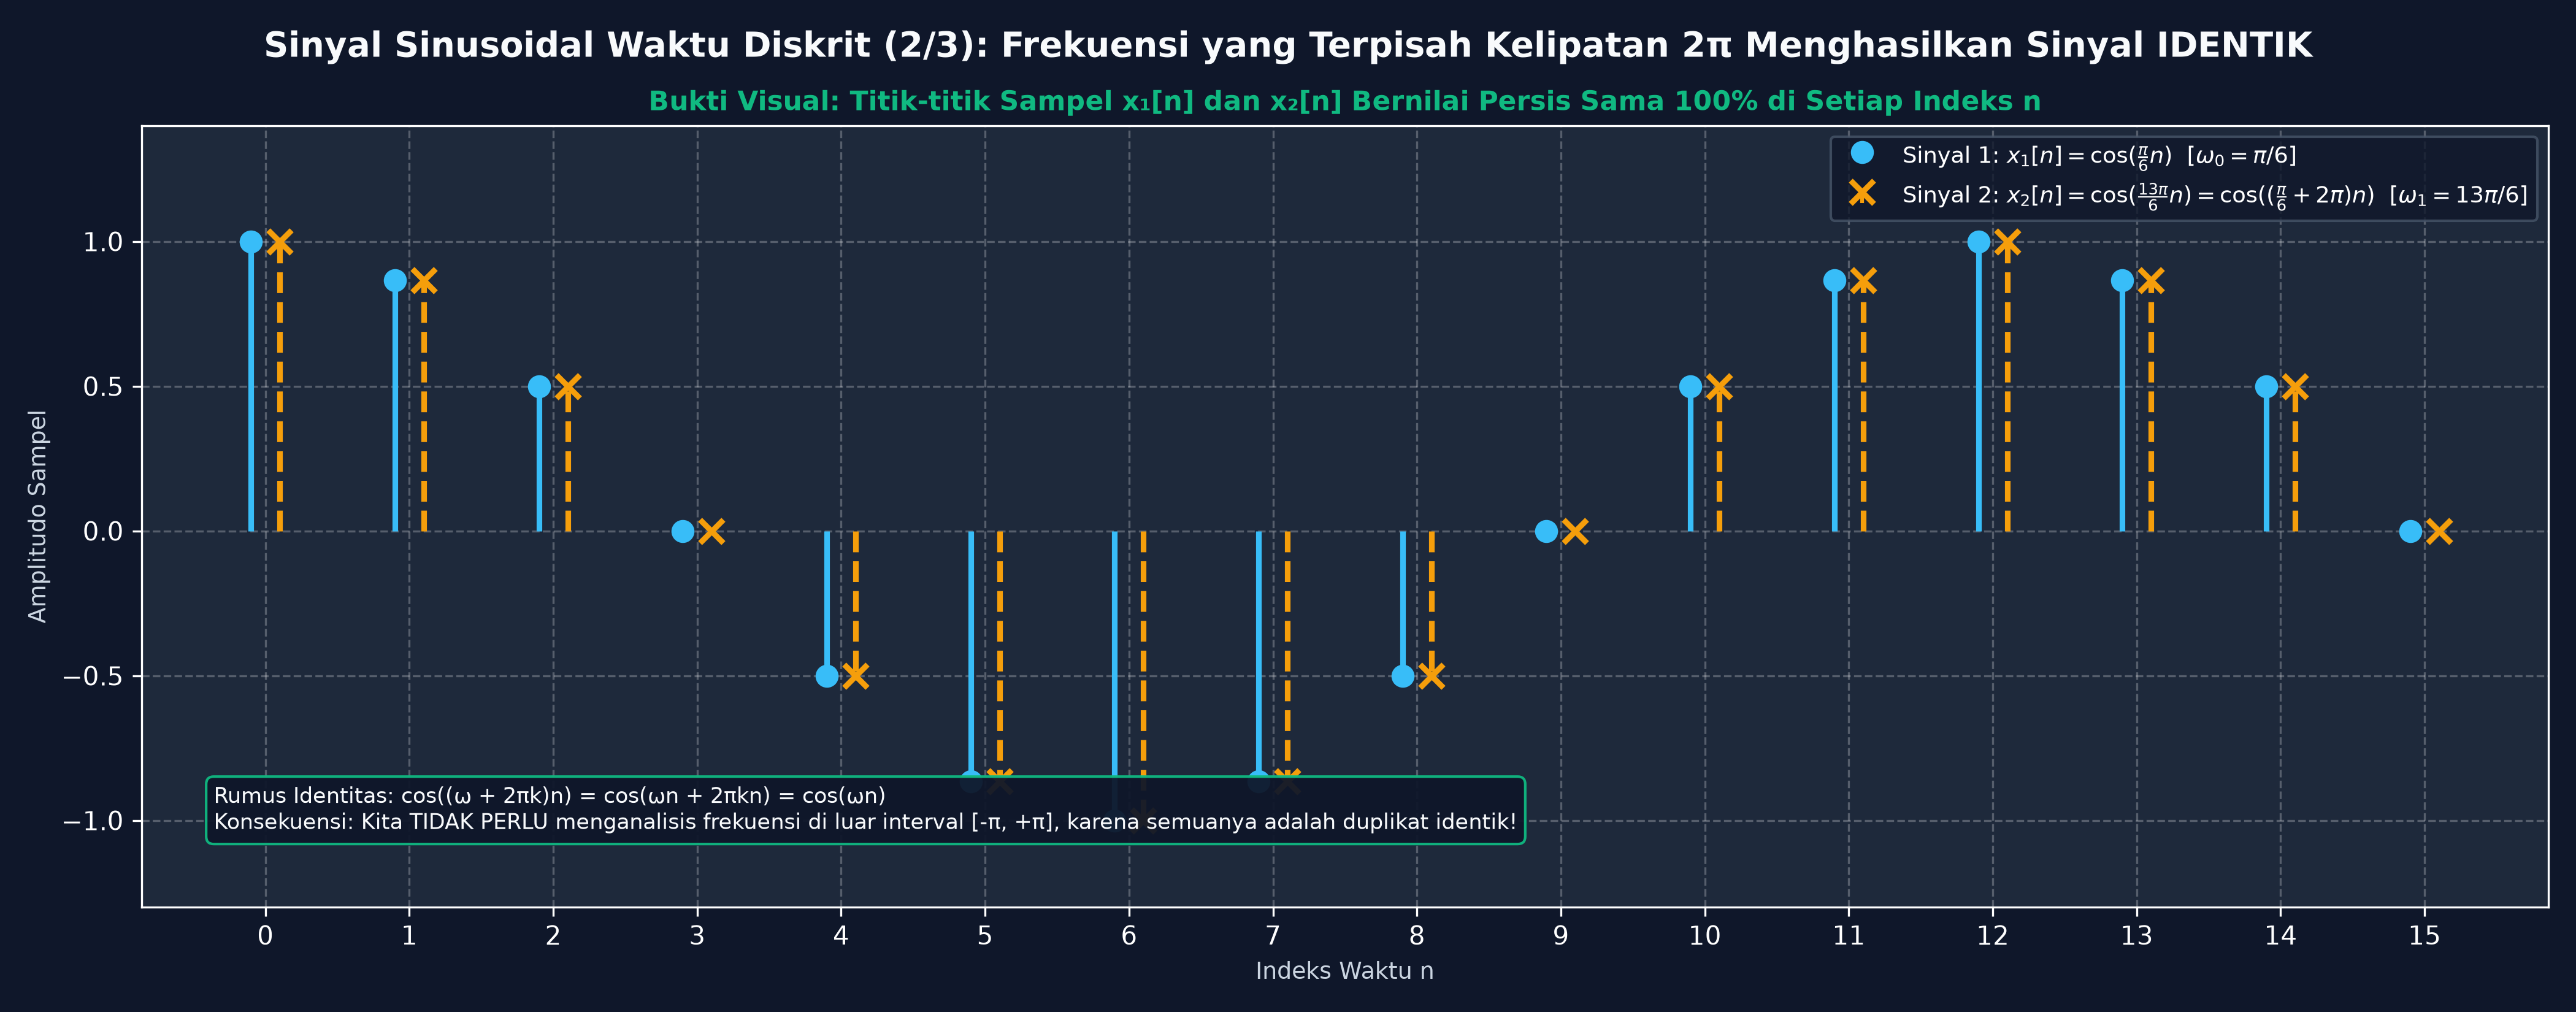
\includegraphics[width=0.92\linewidth]{assets/sinus_diskrit_identik_2pi_2.png}
  \captionof{figure}{Bukti identitas visual: Frekuensi sudut $\omega_0 = \pi/6$ ($30^\circ$) dan $\omega_1 = 13\pi/6 = \pi/6 + 2\pi$ ($390^\circ$) menghasilkan titik cuplikan yang menempel sama persis 100\%.}
\end{center}

\begin{analisisbox}[Teorema Kesamaan Frekuensi Diskrit Modulo $2\pi$]
Untuk sembarang bilangan bulat $k \in \mathbb{Z}$:
\begin{equation}
\cos((\omega + 2\pi k)n + \theta) = \cos(\omega n + 2\pi k n + \theta) = \cos(\omega n + \theta + 2\pi(kn)) = \cos(\omega n + \theta)
\end{equation}
\textit{Konsekuensi Fundamental DSP:} Frekuensi diskrit yang terpisah sejauh kelipatan integer $2\pi$ bukan sekadar menghasilkan gelombang mirip, melainkan **benar-benar identik pada seluruh titik sampel $n$**. Oleh sebab itu, seluruh rentang analisis frekuensi digital dunia hanya dibatasi pada **Interval Fundamental**:
\begin{equation}
-\pi \leq \omega \leq +\pi \quad \iff \quad -\frac{1}{2} \leq f \leq +\frac{1}{2}
\end{equation}
\end{analisisbox}

\newpage
\subsection{Sinyal Sinusoidal Waktu-Diskrit: Laju Osilasi Tertinggi pada \texorpdfstring{$\omega = \pi$}{omega = pi} (\texorpdfstring{$f = 1/2$}{f = 1/2})}

\begin{center}
  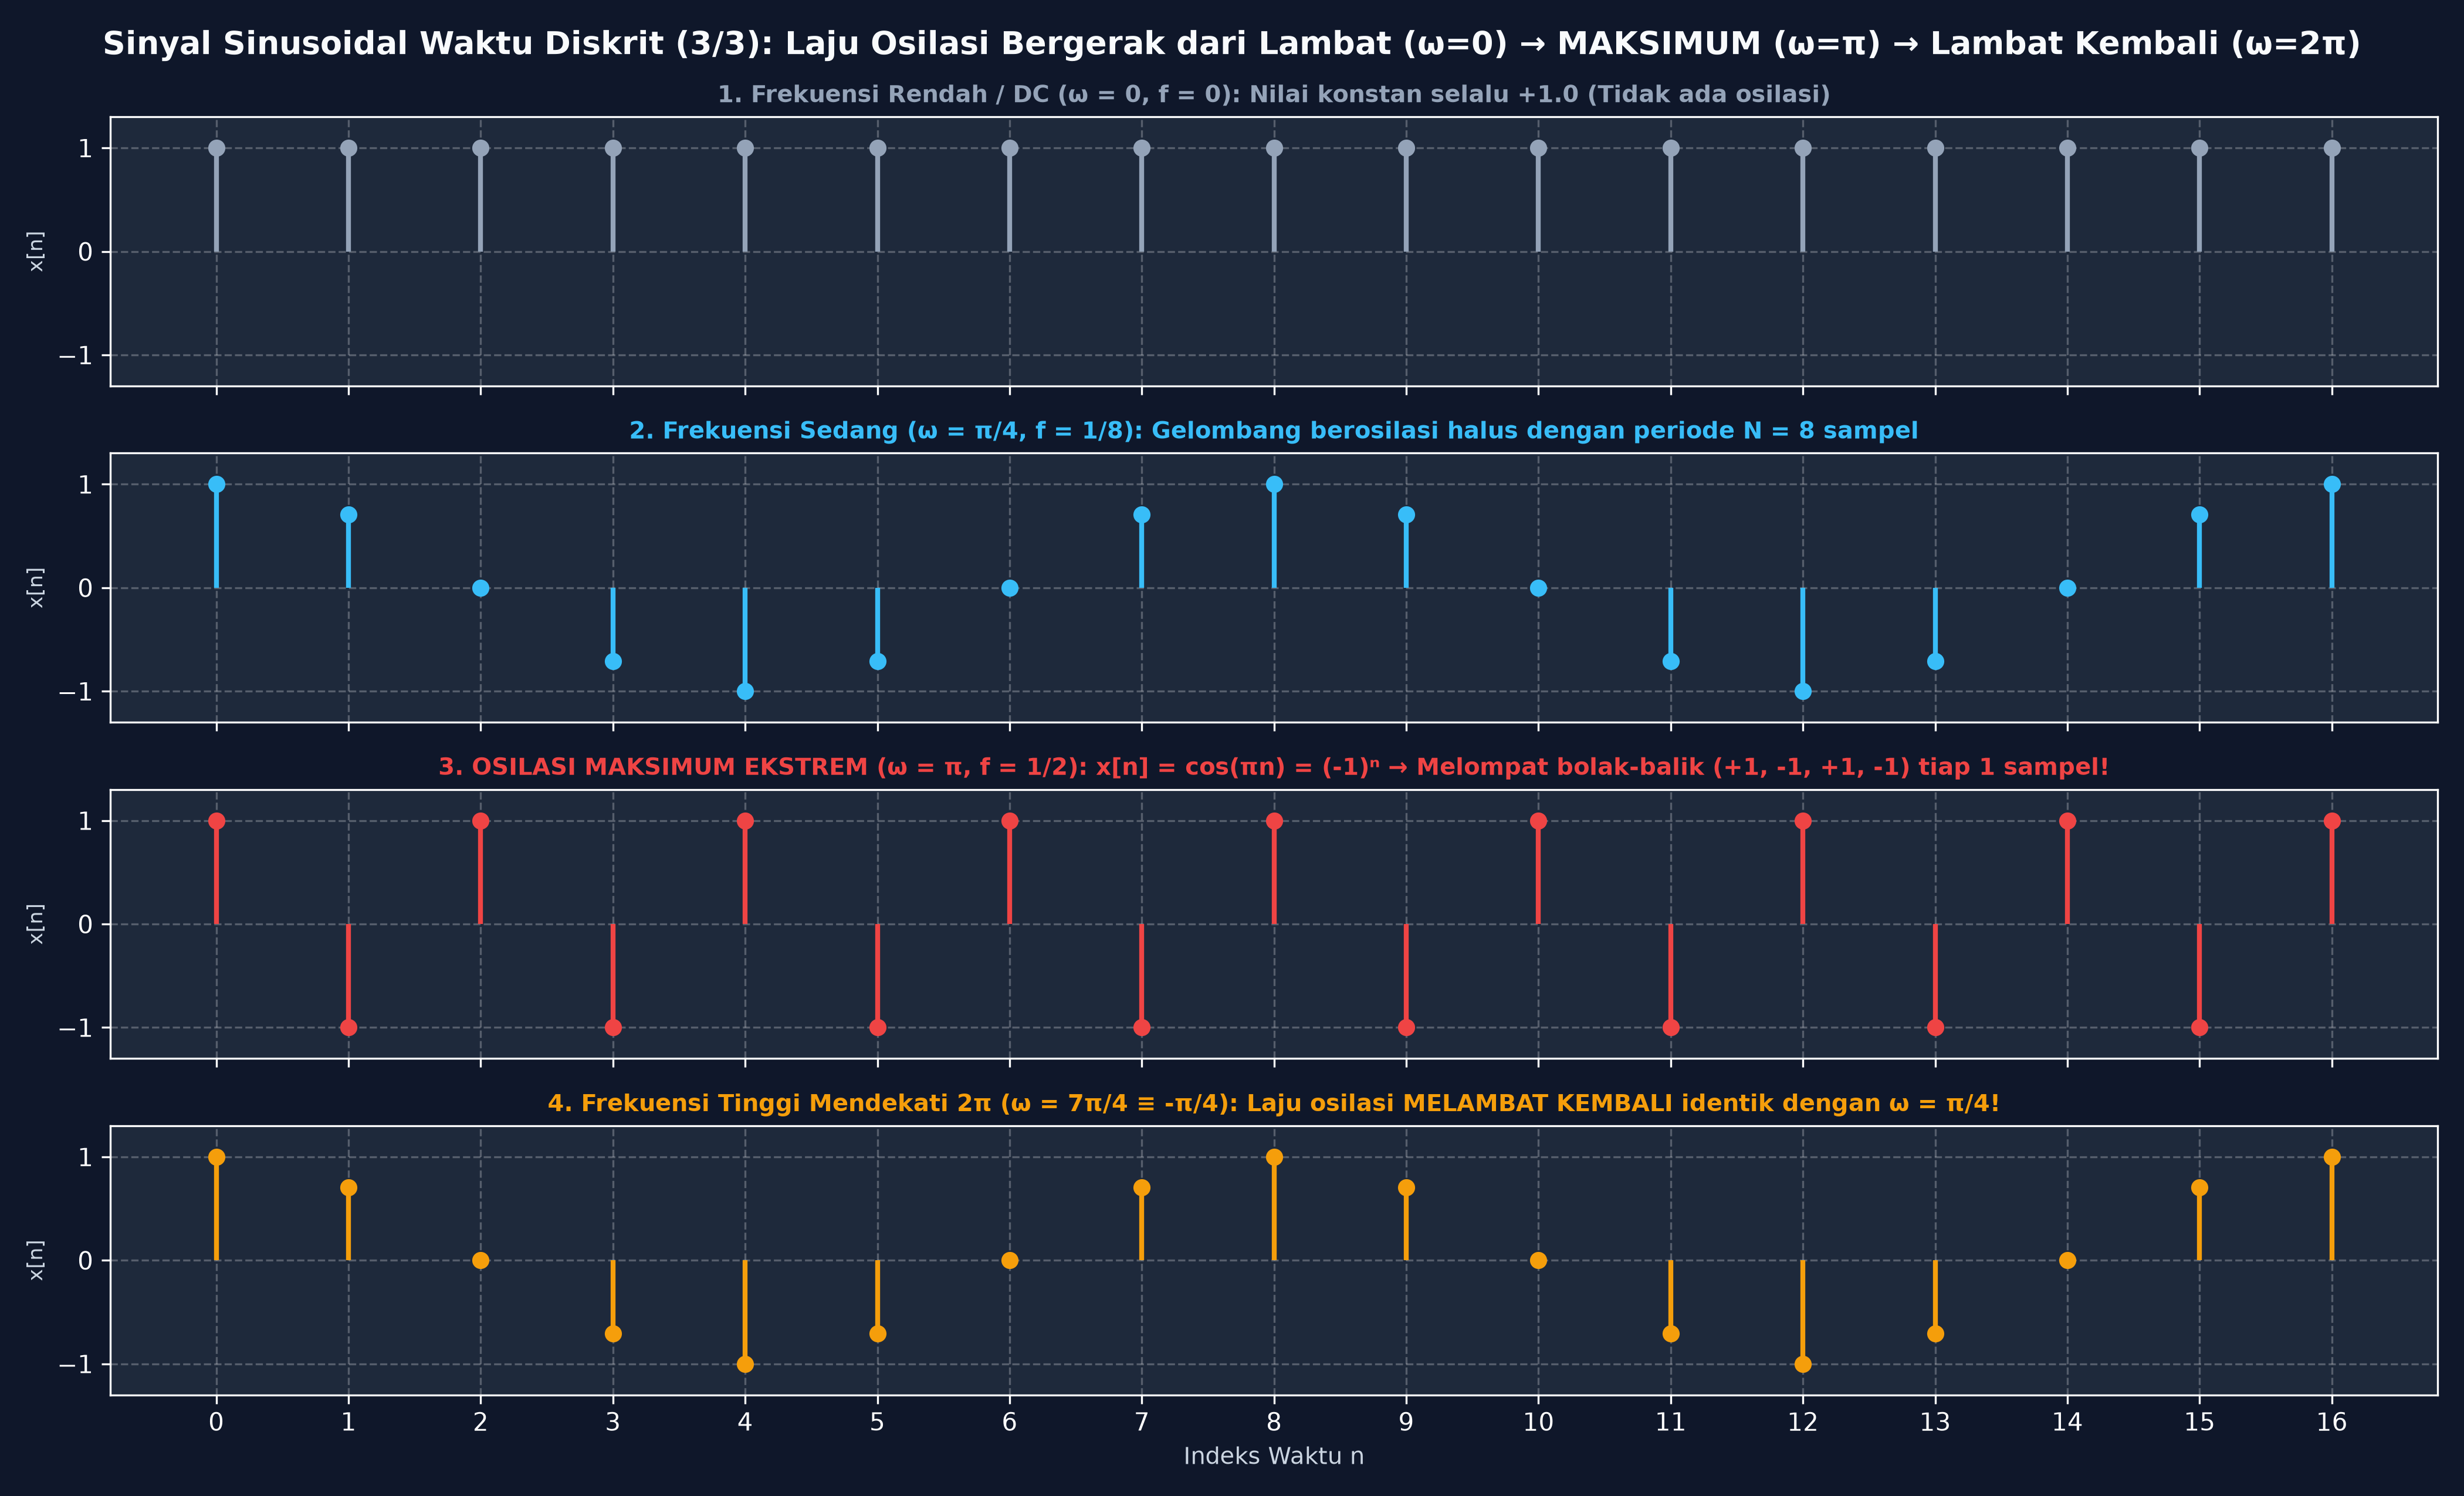
\includegraphics[width=0.95\linewidth]{assets/sinus_diskrit_osilasi_maksimum_3.png}
  \captionof{figure}{Evolusi laju osilasi diskrit: Osilasi nol DC ($\omega = 0$), osilasi sedang ($\omega = \pi/4$), osilasi MAKSIMUM tertinggi ($\omega = \pi$), dan perlambatan semu saat $\omega = 7\pi/4$.}
\end{center}

\begin{analisisbox}[Dekomposisi Laju Osilasi Sinyal Diskrit pada 4 Titik Spektrum]
\begin{enumerate}[leftmargin=*]
  \item \textbf{Titik 1 — Frekuensi Nol / DC ($\omega = 0, f = 0$):}  
  $x[n] = \cos(0 \cdot n) = +1.0, \forall n$. Sinyal berupa garis horizontal konstan tanpa perubahan dinamis.

  \item \textbf{Titik 2 — Frekuensi Menengah ($\omega = \pi/4, f = 1/8$):}  
  Sinyal berosilasi harmonik mulus dengan periode fundamental $N = 8$ sampel per siklus gelombang.

  \item \textbf{Titik 3 — LAJU OSILASI TERTINGGI MAKSIMUM DI DUNIA DIGITAL ($\omega = \pi, f = 1/2$):}  
  \begin{equation}
  x[n] = \cos(\pi n) = (-1)^n = \{+1, -1, +1, -1, +1, -1, \dots\}
  \end{equation}
  Perhatikan titik-titik sampel merah: Sinyal melompat ekstrem dari nilai puncak tertinggi $+1$ ke lembah terendah $-1$ **di setiap 1 perpindahan sampel ($n \to n+1$)**. Ini adalah laju fluktuasi tercepat yang secara matematis dan fisis mungkin terjadi pada sistem waktu-diskrit.

  \item \textbf{Titik 4 — Frekuensi Tinggi Melampaui $\pi$ ($\omega = 7\pi/4 \equiv -\pi/4$):}  
  Ketika frekuensi sudut dinaikkan melampaui $\pi$ menuju $2\pi$, laju osilasi **JUSTRU MELAMBAT KEMBALI**:
  \begin{equation}
  \cos\left(\frac{7\pi}{4} n\right) = \cos\left(\left(2\pi - \frac{\pi}{4}\right)n\right) = \cos\left(-\frac{\pi}{4} n\right) = \cos\left(\frac{\pi}{4} n\right)
  \end{equation}
  Gelombang ini persis identik dengan sinyal frekuensi rendah $\omega = \pi/4$. Fenomena ini membuktikan bahwa batas kecepatan osilasi digital mutlak terkunci di $\omega = \pi$.
\end{enumerate}
\end{analisisbox}

\newpage
% =========================================================================
\section{Studi Kasus \& Contoh Perhitungan Komprehensif Terpadu}
% =========================================================================

Untuk menyatukan pemahaman holistik dari seluruh subbab yang telah dipelajari (**Subbab 1.1 hingga Subbab 1.5**), berikut disajikan sebuah rancang bangun dan komputasi analitis dari sistem instrumentasi industri nyata:

\begin{studiukasusbox}[Grand Problem: Desain Sistem Telemetri Biomedis Multikanal Cerdas (Bio-DSP System)]
\textbf{Deskripsi Sistem:}\\
Sebuah sistem instrumentasi biomedis dirancang untuk memonitor sinyal bio-elektrik jantung pasien. Sistem ini mengintegrasikan rantai fisik sensorik, struktur data multikanal, penapisan filter LTI, digitalisasi ADC kuantisasi resolusi tinggi, serta analisis harmonisa frekuensi diskrit.
\end{studiukasusbox}

\vspace{0.3cm}
\subsection{Spesifikasi \& Parameter Matematis Sistem}

\begin{enumerate}[leftmargin=*]
  \item \textbf{Rantai Fisik \& Sensorik (Subbab 1.1):}  
  Tiga elektroda sensor bio-potensial $Ag/AgCl$ ($M = 3$ kanal) merekam sinyal elektrofisiologis kontinu pasien yang terkontaminasi oleh interferensi derau jala-jala listrik $50\text{ Hz}$ dan osilasi pernapasan respirasi lambat $0.2\text{ Hz}$:
  \begin{align}
  x_1(t) &= 3.0 \cos(2\pi \cdot 10 t) + 1.2 \cos(2\pi \cdot 50 t) + 0.8 \sin(2\pi \cdot 0.2 t) \quad [\text{Volt}] \\
  x_2(t) &= 2.5 \cos(2\pi \cdot 10 t - \pi/6) + 1.2 \cos(2\pi \cdot 50 t) + 0.4 \sin(2\pi \cdot 0.2 t) \quad [\text{Volt}] \\
  x_3(t) &= 1.8 \cos(2\pi \cdot 10 t + \pi/4) + 1.2 \cos(2\pi \cdot 50 t) - 0.5 \sin(2\pi \cdot 0.2 t) \quad [\text{Volt}]
  \end{align}

  \item \textbf{Struktur Data Multikanal (Subbab 1.3):}  
  Sinyal multikanal diorganisasikan ke dalam matriks spasio-temporal $\mathbf{X}(t) \in \mathbb{R}^{3 \times N}$. Dilakukan operasi pembobotan spasial diferensial untuk membatalkan komponen *common-mode noise* $50\text{ Hz}$ dengan vektor bobot $\mathbf{w} = [1, -1, 0]^T$:
  \begin{equation}
  s_a(t) = \mathbf{w}^T \mathbf{x}(t) = x_1(t) - x_2(t)
  \end{equation}

  \item \textbf{Spesifikasi ADC \& Digitalisasi (Subbab 1.2 \& 1.4):}
  \begin{itemize}
    \item Frekuensi Sampling Sistem: $F_s = 200\text{ Hz}$ ($T_s = 5\text{ ms} = 0.005\text{ s}$).
    \item Terdapat komponen derau interferensi frekuensi tinggi liar tak terfilter pada $f_{\text{noise}} = 230\text{ Hz}$ dengan persamaan $v_{\text{noise}}(t) = 0.5 \cos(2\pi \cdot 230 t)$.
    \item Konverter ADC Uniform 4-Bit ($B = 4\text{ bit} \implies L = 16\text{ level}$), dengan rentang tegangan dinamis $V_{\text{min}} = -4.0\text{ V}$ hingga $V_{\text{maks}} = +4.0\text{ V}$ ($V_{\text{range}} = 8.0\text{ V}$).
  \end{itemize}

  \item \textbf{Filter Digital Pemroses LTI (Subbab 1.1 \& 1.3):}  
  Sinyal tercuplik $s[n]$ dilewatkan ke sebuah filter rata-rata bergerak 3-titik (*3-Point Moving Average Filter*):
  \begin{equation}
  y[n] = \frac{1}{3}s[n] + \frac{1}{3}s[n-1] + \frac{1}{3}s[n-2]
  \end{equation}
\end{enumerate}

\newpage
\subsection{Penyelesaian Komputasi Analitis Langkah-demi-Langkah}

\subsubsection{Langkah 1: Reduksi Multikanal \& Analisis Parameter Gelombang (Subbab 1.1 \& 1.3)}
Hitung sinyal hasil kombinasi spasial $s_a(t) = x_1(t) - x_2(t)$:
\begin{align*}
s_a(t) &= \left[ 3.0 \cos(20\pi t) + 1.2 \cos(100\pi t) + 0.8 \sin(0.4\pi t) \right] \\
&\quad - \left[ 2.5 \cos(20\pi t - \pi/6) + 1.2 \cos(100\pi t) + 0.4 \sin(0.4\pi t) \right] \\
&= \underbrace{\left[ 3.0 \cos(20\pi t) - 2.5 \cos(20\pi t - \pi/6) \right]}_{\text{Komponen Jantung 10 Hz}} + \underbrace{[1.2 - 1.2]\cos(100\pi t)}_{\mathbf{0\text{ (Derau 50 Hz Lenyap!)}}} + \underbrace{0.4 \sin(0.4\pi t)}_{\text{Respirasi 0.2 Hz}}
\end{align*}
Gunakan identitas trigonometri fasor untuk menyederhanakan komponen $10\text{ Hz}$:
\begin{align*}
2.5 \cos(20\pi t - \pi/6) &= 2.5 \left[ \cos(20\pi t)\cos(\pi/6) + \sin(20\pi t)\sin(\pi/6) \right] \\
&= 2.5 \left[ \frac{\sqrt{3}}{2} \cos(20\pi t) + \frac{1}{2} \sin(20\pi t) \right] \approx 2.165 \cos(20\pi t) + 1.250 \sin(20\pi t)
\end{align*}
Maka:
\begin{equation}
s_{10\text{Hz}}(t) = (3.0 - 2.165)\cos(20\pi t) - 1.250 \sin(20\pi t) = 0.835 \cos(20\pi t) - 1.250 \sin(20\pi t)
\end{equation}
Amplitudo resultan $A_R$ dan sudut fase $\phi_R$:
\begin{equation}
A_R = \sqrt{(0.835)^2 + (-1.250)^2} = \sqrt{0.6972 + 1.5625} = \sqrt{2.2597} \approx \mathbf{1.503\text{ Volt}}
\end{equation}
\begin{equation}
\phi_R = \operatorname{atan2}(-1.250, 0.835) \approx -56.27^\circ \approx -0.982\text{ rad}
\end{equation}
Persamaan analitis bersih sinyal kontinu yang masuk ke ADC (termasuk derau liar $230\text{ Hz}$):
\begin{equation}
s_{\text{total}}(t) = 1.503 \cos(2\pi \cdot 10 t - 0.982) + 0.4 \sin(2\pi \cdot 0.2 t) + 0.5 \cos(2\pi \cdot 230 t)
\end{equation}

\vspace{0.2cm}
\subsubsection{Langkah 2: Evaluasi Nyquist, Identifikasi Aliasing, dan Pemetaan Frekuensi Diskrit (Subbab 1.2 \& 1.5)}
\begin{enumerate}[leftmargin=*]
  \item \textbf{Analisis Frekuensi Nyquist:}  
  Frekuensi sampling $F_s = 200\text{ Hz} \implies$ Frekuensi Nyquist ($f_{\text{fold}}$) adalah:
  \begin{equation}
  f_{\text{fold}} = \frac{F_s}{2} = \frac{200\text{ Hz}}{2} = \mathbf{100\text{ Hz}}
  \end{equation}
  \item \textbf{Evaluasi Komponen $F_1 = 10\text{ Hz}$ dan $F_2 = 0.2\text{ Hz}$:}  
  Karena $F_1, F_2 < 100\text{ Hz}$, kedua komponen berada di dalam pita Nyquist dan disampling secara aman bebas aliasing. Frekuensi digitalnya:
  \begin{equation}
  \omega_1 = \frac{2\pi F_1}{F_s} = \frac{2\pi \cdot 10}{200} = \mathbf{\frac{\pi}{10}\ \text{rad/sampel}}, \qquad f_1 = \frac{10}{200} = \mathbf{\frac{1}{20}\ \text{siklus/sampel}}
  \end{equation}
  \begin{equation}
  \omega_2 = \frac{2\pi F_2}{F_s} = \frac{2\pi \cdot 0.2}{200} = \mathbf{\frac{\pi}{500}\ \text{rad/sampel}}, \qquad f_2 = \frac{0.2}{200} = \mathbf{\frac{1}{1000}\ \text{siklus/sampel}}
  \end{equation}
  
  \item \textbf{Evaluasi Aliasing Komponen Liar $F_3 = 230\text{ Hz}$:}  
  Karena $F_3 = 230\text{ Hz} > 100\text{ Hz}$, terjadi pelanggaran kriteria Nyquist (*Under-sampling*). Komponen ini terlipat ke frekuensi semu alias:
  \begin{equation}
  f_{\text{alias}} = |F_3 - 1 \cdot F_s| = |230\text{ Hz} - 200\text{ Hz}| = \mathbf{30\text{ Hz}}
  \end{equation}
  Frekuensi sudut diskrit aliasnya:
  \begin{equation}
  \omega_{\text{alias}} = \frac{2\pi \cdot 30}{200} = \mathbf{\frac{3\pi}{10}\ \text{rad/sampel}} \quad \left(f_{\text{alias}} = \frac{3}{20}\right)
  \end{equation}

  \item \textbf{Uji Periodisitas Diskrit (Subbab 1.5.4):}
  \begin{itemize}
    \item Untuk $\omega_1$: $f_1 = 1/20 \in \mathbb{Q} \implies$ **Periodik** dengan periode fundamental $N_1 = 20\text{ sampel}$.
    \item Untuk $\omega_2$: $f_2 = 1/1000 \in \mathbb{Q} \implies$ **Periodik** dengan periode fundamental $N_2 = 1000\text{ sampel}$.
    \item Untuk $\omega_{\text{alias}}$: $f_{\text{alias}} = 3/20 \in \mathbb{Q} \implies$ **Periodik** dengan periode fundamental $N_3 = \frac{20}{\gcd(3,20)} = 20\text{ sampel}$.
    \item **Periode Fundamental Total Sinyal Campuran:**
    \begin{equation}
    N_{\text{total}} = \operatorname{KPK}(N_1, N_2, N_3) = \operatorname{KPK}(20, 1000, 20) = \mathbf{1000\text{ sampel}} \quad (\text{setara } 5.0\text{ detik})
    \end{equation}
  \end{itemize}
\end{enumerate}

\newpage
\subsubsection{Langkah 3: Perhitungan Kuantisasi ADC 4-Bit \& Kinerja Derau SQNR (Subbab 1.2 \& 1.4)}
\begin{enumerate}[leftmargin=*]
  \item \textbf{Parameter Kuantisasi ADC 4-Bit ($B = 4, L = 16$ level):}
  \begin{equation}
  \Delta = \frac{V_{\text{maks}} - V_{\text{min}}}{2^B} = \frac{+4.0\text{ V} - (-4.0\text{ V})}{16} = \frac{8.0\text{ V}}{16} = \mathbf{0.50\text{ Volt / step}}
  \end{equation}
  Batas level representasi kuantisasi $V_q(k) = -4.0 + (k + 0.5)\Delta = -3.75 + k(0.50)\text{ V}$ untuk $k = 0, 1, \dots, 15$.
  \item \textbf{Daya Derau Kuantisasi Teoritis:}
  \begin{equation}
  P_e = \sigma_e^2 = \frac{\Delta^2}{12} = \frac{(0.50)^2}{12} = \frac{0.25}{12} = \mathbf{0.020833\ \text{V}^2}
  \end{equation}
  \item \textbf{SQNR Maksimum Teoritis (Skala Penuh $A = 4.0\text{ V}$):}
  \begin{equation}
  \text{SQNR}_{\text{teoritis}} = 6.02 \cdot B + 1.76 = 6.02(4) + 1.76 = 24.08 + 1.76 = \mathbf{25.84\text{ dB}}
  \end{equation}
\end{enumerate}

\vspace{0.2cm}
\textbf{Kalkulasi Numerik Pelacakan 4 Sampel Pertama ($n=0, 1, 2, 3$):}\\
Sinyal diskrit masukan sebelum kuantisasi:
\begin{equation}
s[n] = 1.503 \cos\left(\frac{\pi}{10}n - 0.982\right) + 0.4 \sin\left(\frac{\pi}{500}n\right) + 0.5 \cos\left(\frac{3\pi}{10}n\right)
\end{equation}
\begin{itemize}[leftmargin=*]
  \item \textbf{Sampel $n=0$ ($t = 0.000\text{ s}$):}
  \begin{align*}
  s[0] &= 1.503 \cos(-0.982) + 0.4 \sin(0) + 0.5 \cos(0) \\
  &= 1.503(0.5552) + 0 + 0.5(1) = 0.8345 + 0.5 = \mathbf{+1.3345\text{ V}}
  \end{align*}
  \textit{Kuantisasi:} Step index $k = \left\lfloor \frac{1.3345 - (-4.0)}{0.5} \right\rfloor = \lfloor 10.669 \rfloor = 10 \implies$ \textbf{Step 11} (\texttt{1010}).\\
  Level representasi $V_q = -4.0 + 10.5(0.5) = \mathbf{+1.250\text{ V}}$. Galat kuantisasi: $e_q[0] = 1.250 - 1.3345 = \mathbf{-0.0845\text{ V}}$.

  \item \textbf{Sampel $n=1$ ($t = 0.005\text{ s}$):}
  \begin{align*}
  s[1] &= 1.503 \cos\left(\frac{\pi}{10} - 0.982\right) + 0.4 \sin\left(\frac{\pi}{500}\right) + 0.5 \cos\left(\frac{3\pi}{10}\right) \\
  &= 1.503(0.7856) + 0.0025 + 0.2939 = \mathbf{+1.4772\text{ V}}
  \end{align*}
  \textit{Kuantisasi:} Step index $k = \lfloor 10.954 \rfloor = 10 \implies$ \textbf{Step 11} (\texttt{1010}), $V_q = \mathbf{+1.250\text{ V}}$.\\
  Galat kuantisasi: $e_q[1] = 1.250 - 1.4772 = \mathbf{-0.2272\text{ V}}$.

  \item \textbf{Sampel $n=2$ ($t = 0.010\text{ s}$):}
  \begin{align*}
  s[2] &= 1.503 \cos\left(\frac{2\pi}{10} - 0.982\right) + 0.4 \sin\left(\frac{2\pi}{500}\right) + 0.5 \cos\left(\frac{6\pi}{10}\right) \\
  &= 1.503(0.9377) + 0.0050 - 0.1545 = \mathbf{+1.2599\text{ V}}
  \end{align*}
  \textit{Kuantisasi:} Step index $k = \lfloor 10.520 \rfloor = 10 \implies$ \textbf{Step 11} (\texttt{1010}), $V_q = \mathbf{+1.250\text{ V}}$.\\
  Galat kuantisasi: $e_q[2] = 1.250 - 1.2599 = \mathbf{-0.0099\text{ V}}$.

  \item \textbf{Sampel $n=3$ ($t = 0.015\text{ s}$):}
  \begin{align*}
  s[3] &= 1.503 \cos\left(\frac{3\pi}{10} - 0.982\right) + 0.4 \sin\left(\frac{3\pi}{500}\right) + 0.5 \cos\left(\frac{9\pi}{10}\right) \\
  &= 1.503(0.9992) + 0.0075 - 0.4755 = \mathbf{+1.0338\text{ V}}
  \end{align*}
  \textit{Kuantisasi:} Step index $k = \lfloor 10.068 \rfloor = 10 \implies$ \textbf{Step 11} (\texttt{1010}), $V_q = \mathbf{+1.250\text{ V}}$.\\
  Galat kuantisasi: $e_q[3] = 1.250 - 1.0338 = \mathbf{+0.2162\text{ V}}$.
\end{itemize}

\vspace{0.2cm}
\textbf{Aliran Bitstream Serial 4-Bit yang Dihasilkan:}
\[
\mathbf{\text{Frame Bitstream [4 Sampel]}} = \mathbf{\underbrace{1010}_{n=0} \ \underbrace{1010}_{n=1} \ \underbrace{1010}_{n=2} \ \underbrace{1010}_{n=3}} \quad (16\text{ bit})
\]

\newpage
\subsubsection{Langkah 4: Pemrosesan Filter LTI \& Uji Karakteristik Sistem (Subbab 1.1 \& 1.3)}
Sinyal terkuantisasi $s_q[n]$ diproses oleh filter rata-rata bergerak 3-titik:
\begin{equation}
y[n] = \frac{1}{3} s_q[n] + \frac{1}{3} s_q[n-1] + \frac{1}{3} s_q[n-2]
\end{equation}

\textbf{1. Verifikasi 4 Sifat Karakteristik Sistem Filter:}
\begin{itemize}[leftmargin=*]
  \item \textbf{Uji Linearitas:} Misalkan $s_q[n] = a x_1[n] + b x_2[n]$:
  \begin{align*}
  y[n] &= \frac{1}{3}(a x_1[n] + b x_2[n]) + \frac{1}{3}(a x_1[n-1] + b x_2[n-1]) + \frac{1}{3}(a x_1[n-2] + b x_2[n-2]) \\
  &= a \left[\frac{1}{3}x_1[n] + \frac{1}{3}x_1[n-1] + \frac{1}{3}x_1[n-2]\right] + b \left[\frac{1}{3}x_2[n] + \frac{1}{3}x_2[n-1] + \frac{1}{3}x_2[n-2]\right] \\
  &= a y_1[n] + b y_2[n] \quad \mathbf{(\text{Terbukti Linier!})}
  \end{align*}
  \item \textbf{Uji Time-Invariance:} Jika input digeser $s_q[n-n_0]$, output menjadi $\frac{1}{3}\sum_{k=0}^2 s_q[n-n_0-k] = y[n-n_0] \quad \mathbf{(\text{Terbukti Time-Invariant!})}$.
  \item \textbf{Uji Kausalitas:} Respon impuls sistem adalah $h[n] = \frac{1}{3}\delta[n] + \frac{1}{3}\delta[n-1] + \frac{1}{3}\delta[n-2]$. Karena $h[n] = 0$ untuk seluruh $n < 0$, maka sistem \textbf{Terbukti Kausal}.
  \item \textbf{Uji Stabilitas BIBO:}
  \begin{equation}
  S_h = \sum_{n=-\infty}^{\infty} |h[n]| = |h[0]| + |h[1]| + |h[2]| = \frac{1}{3} + \frac{1}{3} + \frac{1}{3} = \mathbf{1.0 < \infty} \quad \mathbf{(\text{Terbukti Stabil BIBO!})}
  \end{equation}
\end{itemize}

\vspace{0.2cm}
\textbf{2. Perhitungan Respon Frekuensi Filter terhadap Derau Alias 30 Hz ($3\pi/10$):}
\begin{equation}
H(e^{j\omega}) = \sum_{n=0}^2 h[n] e^{-j\omega n} = \frac{1}{3}\left( 1 + e^{-j\omega} + e^{-j2\omega} \right) = \frac{1}{3} e^{-j\omega} \left( 1 + 2\cos(\omega) \right)
\end{equation}
Magnitudo penguatan filter $|H(e^{j\omega})| = \frac{1}{3}|1 + 2\cos(\omega)|$.
\begin{itemize}[leftmargin=*]
  \item Pada sinyal jantung $\omega_1 = \frac{\pi}{10} = 18^\circ$:
  \begin{equation}
  |H(e^{j\pi/10})| = \frac{1}{3}|1 + 2\cos(18^\circ)| = \frac{1}{3}|1 + 2(0.9511)| \approx \mathbf{0.9674\ (-0.29\text{ dB})} \implies \text{Lolos Utuh!}
  \end{equation}
  \item Pada derau liar alias $\omega_{\text{alias}} = \frac{3\pi}{10} = 54^\circ$:
  \begin{equation}
  |H(e^{j3\pi/10})| = \frac{1}{3}|1 + 2\cos(54^\circ)| = \frac{1}{3}|1 + 2(0.5878)| \approx \mathbf{0.7252\ (-2.79\text{ dB})} \implies \text{Tereduksi!}
  \end{equation}
\end{itemize}

\vspace{0.2cm}
\textbf{3. Kalkulasi Numerik Keluaran Filter $y[2]$:}
Dengan asumsi kondisi diam awal $s_q[-1] = 0, s_q[-2] = 0$:
\begin{equation}
y[2] = \frac{1}{3}s_q[2] + \frac{1}{3}s_q[1] + \frac{1}{3}s_q[0] = \frac{1}{3}(1.250) + \frac{1}{3}(1.250) + \frac{1}{3}(1.250) = \mathbf{1.250\text{ Volt}}
\end{equation}

\vspace{0.3cm}
\begin{tcolorbox}[colback=accent!10, colframe=accent, arc=2mm, title=\textbf{Kesimpulan Grand Synthesis Subbab 1.1 - 1.5}]
Studi kasus ini secara matematis membuktikan integrasi end-to-end:
1. **1.1:** Pemodelan transduksi bio-potensial, derau termal, dan eliminasi interferensi fasor fase kuadratur.
2. **1.2:** Laju sampling $F_s$, pencegahan aliasing Nyquist, serta kuantisasi uniform $4$-bit dengan presisi $\Delta = 0.5\text{ V}$.
3. **1.3:** Aljabar linear multikanal matriks spasio-temporal dan dekomposisi sinyal elementer.
4. **1.4:** Topologi sinyal digital kuadran-4 dan model derau kuantisasi aditif berdaya $\sigma_e^2 = \Delta^2/12$.
5. **1.5:** Periodisitas rasional frekuensi diskrit $f = k/N$, identitas kesamaan modulo $2\pi$, dan penapisan magnitudo filter LTI.
\end{tcolorbox}

\newpage
% =========================================================================
\section{Glosarium Ringkas Istilah Kunci Persinyalan}
% =========================================================================

\subsection{Konsep Dasar \& Paradigma}
\begin{table}[h!]
\centering
\small
\begin{tabularx}{\textwidth}{l>{\raggedright\arraybackslash}X}
\toprule
\textbf{Istilah} & \textbf{Definisi \& Konsep Kunci} \\
\midrule
\textbf{Sinyal (\textit{Signal})} & Besaran fisik pembawa informasi yang nilainya berubah sebagai fungsi dari satu atau lebih variabel bebas (tegangan, tekanan akustik, suhu). \\
\textbf{Sistem (\textit{System})} & Entitas fisik atau algoritma komputasi yang memetakan sinyal masukan (*excitation*) menjadi sinyal keluaran (*response*). \\
\textbf{ASP (\textit{Analog Signal Processing})} & Pemrosesan sinyal kontinu langsung menggunakan komponen perangkat keras fisik ($R, L, C, \text{Op-Amp}$) diatur oleh persamaan diferensial LCCDE. \\
\textbf{DSP (\textit{Digital Signal Processing})} & Pemrosesan sinyal diskrit numerik menggunakan algoritma aljabar pada prosesor digital diatur oleh persamaan beda LCCDDE. \\
\textbf{Sensor / Transduser} & Perangkat konversi energi yang mengubah fenomena fisis non-listrik menjadi fluktuasi sinyal tegangan/arus listrik proporsional. \\
\bottomrule
\end{tabularx}
\end{table}

\subsection{Anatomi \& Parameter Gelombang}
\begin{table}[h!]
\centering
\small
\begin{tabularx}{\textwidth}{l>{\raggedright\arraybackslash}X}
\toprule
\textbf{Istilah} & \textbf{Definisi \& Konsep Kunci} \\
\midrule
\textbf{Amplitudo ($A$)} & Simpangan puncak ekstrem gelombang dari titik nol, menentukan daya rata-rata $P = A^2/2$ dan tegangan efektif $V_{\text{rms}} = A/\sqrt{2}$. \\
\textbf{Frekuensi ($f, F$)} & Jumlah osilasi siklus gelombang lengkap dalam 1 detik ($\text{Hertz} = \text{s}^{-1}$). \\
\textbf{Periode ($T$)} & Interval waktu minimum yang diperlukan untuk menyelesaikan 1 siklus osilasi periodik penuh ($T = 1/f$). \\
\textbf{Frekuensi Sudut ($\Omega, \omega$)} & Laju kecepatan rotasi fase gelombang ($\Omega = 2\pi F\text{ rad/s}$ untuk kontinu; $\omega = 2\pi f\text{ rad/sampel}$ untuk diskrit). \\
\textbf{Fase Awal ($\phi, \theta$)} & Posisi sudut mula gelombang pada $t = 0$, setara dengan pergeseran translasi waktu $\Delta t = -\phi/\Omega$. \\
\bottomrule
\end{tabularx}
\end{table}

\subsection{Proses Digitalisasi \& ADC}
\begin{table}[h!]
\centering
\small
\begin{tabularx}{\textwidth}{l>{\raggedright\arraybackslash}X}
\toprule
\textbf{Istilah} & \textbf{Definisi \& Konsep Kunci} \\
\midrule
\textbf{ADC (\textit{A/D Converter})} & Subsistem pengubah sinyal kontinu analog menjadi kata-kata biner digital melalui rantai sampling, kuantisasi, dan encoding. \\
\textbf{Pencuplikan (\textit{Sampling})} & Proses modulasi sinyal kontinu dengan deretan pulsa Dirac pada interval waktu berkala $T_s = 1/F_s$. \\
\textbf{Teorema Nyquist} & Syarat batas absolut bebas aliasing: frekuensi sampling wajib memenuhi $F_s \ge 2 f_{\max}$. \\
\textbf{Aliasing} & Distorsi lipatan spektral di mana frekuensi di atas $F_s/2$ menyamar menjadi frekuensi rendah palsu $f_{\text{alias}} = |F - k F_s|$. \\
\textbf{Kuantisasi (\textit{Quantization})} & Pembulatan non-linier amplitudo kontinu ke $L = 2^B$ level diskrit terdekat dengan lebar step $\Delta = V_{\text{range}}/2^B$. \\
\textbf{SQNR} & Rasio Daya Sinyal terhadap Derau Kuantisasi berdaya $\sigma_e^2 = \Delta^2/12$, bernilai $\text{SQNR} \approx 6.02 B + 1.76\text{ dB}$. \\
\bottomrule
\end{tabularx}
\end{table}

\subsection{Klasifikasi Sinyal \& Karakteristik Sistem}
\begin{table}[h!]
\centering
\small
\begin{tabularx}{\textwidth}{l>{\raggedright\arraybackslash}X}
\toprule
\textbf{Istilah} & \textbf{Definisi \& Konsep Kunci} \\
\midrule
\textbf{Sinyal Digital Murni} & Sinyal pada Kuadran-4 yang berada dalam domain waktu-diskrit ($n \in \mathbb{Z}$) dan bernilai amplitudo diskrit biner ($x_q \in \mathbb{D}_L$). \\
\textbf{Sinyal Multikanal} & Matriks data spasio-temporal $\mathbf{X} \in \mathbb{R}^{M \times N}$ yang dihimpun dari array $M$ sensor serentak. \\
\textbf{Sinyal Multi-Dimensi} & Sinyal yang dipetakan oleh $M$ variabel bebas independen (1D audio, 2D citra, 3D video/MRI, 4D hyperspectral). \\
\textbf{Deterministik vs Stokastik} & Sinyal terprediksi 100\% via formula matematis eksak vs sinyal acak berderau yang dimodelkan via autokorelasi $R_{xx}(\tau)$ dan PSD. \\
\textbf{Linearitas} & Kepatuhan sistem terhadap prinsip superposisi: $\mathcal{T}\{\alpha x_1 + \beta x_2\} = \alpha y_1 + \beta y_2$. \\
\textbf{Time-Invariance} & Kekekalan sifat sistem terhadap pergeseran waktu: $\mathcal{T}\{x[n-n_0]\} = y[n-n_0]$. \\
\textbf{Kausalitas} & Sistem yang responnya tidak mendahului input ($h[n] = 0, \forall n < 0$). \\
\textbf{Stabilitas BIBO} & Jaminan keluaran terbatas untuk masukan terbatas, dicapai jika dan hanya jika $\sum |h[n]| < \infty$. \\
\bottomrule
\end{tabularx}
\end{table}

\vspace{0.6cm}
\begin{center}
\small\itshape\color{gray}
--- Modul Pembelajaran Visual Komprehensif Pengolahan Sinyal Digital (PSD) berstandar industri dan akademis ---
\end{center}

\end{document}
